\documentclass[14pt, a4paper]{book}
\begin{document}

\graphicspath{{../../figures/}}
\section{Data Preparation/LOG}
We are dropping $\Delta\phi(l_1,l_2)$ and $\Delta\phi(l_c,E_T^{miss})$ due the poor agreement between MC and data. The first one is most likely due us not including fake leptons (and also for all non SFOS final states). \todo{I will remove this sentence, but its just so we know}The latter is a problem that PhD. Even is being haunted by. 
There is also the problem of missing variables. For this theis, as shown in Table \ref{tab:paddable_variables}, we will record events with up to three jets in the final state. As mentioned earlier, there isn't 
always three jets in the final state, to mediate this problem I chose to set the $p_T$ to zero for the missing jets and $m_{jj}$ to zero if there are less than two jets, this is something that is physically reasonable as it doesn't violate any conservation laws. 
More problematic however is the $\eta$ and $\phi$ when there aren't jets. To mediate this I've set the values to -999, which has no physical meaning and is impossible to achieve, this I did so it becomes easier for us to identify the jagged arrays further in the network preparation. 
The missing variables is not a problem when making BDTs with XGBoost. There is also another problem, albeit less problematic than the previous ones, with the final states that are not SFOS, as the MC generated background 
on these tend to be lower than the recorded data. The number of events that are not SFOS are minimal though, and we think the reason it doesn't fit the data is because we are not including fake leptons. \todo{something more to add?}

\subsection{Zp Dark Matter dataset}
To train the networks I will utilize two methods\todo{see next comment for the two methods}. The first one being this where the dataset being sent into the ML network will contain every single DM MC sample available. 
So far there are 154 different MC samples, these are based on three theories. A Light Vector (LV), Dark Higgs (DH) and Effective Field Theory (EFT) which produces the WIMP DM particles, and a new theoretical particle, $Z'$, 
that decays into a lepton pair. The three theories are divided further into MC samples with a Light Dark Sector (LDS) and High Dark Sector (HDS) which tells us therange of the Dark Matter candidate mass. 
And lastly it is divided further into more MC samples with different masses for $Z'$. This dataset includes all of these samples such that the network learns Dark Matter in a model independent way.

\subsection{"Ensemble" dataset / Model indepedence}\todo{This subsection and is outdated with our current plan, and this will change when we discuss further how to implement the model-independent aspect.}
Another approach is to make multiple datasets and combine the results of every network into a "big network". This is the second approach which I call ensemble modelling. The thought behind this is that when 
training a network using the full dataset it might only focus on a the more resonant models with fixed masses. Also, every different DM sample has different phenomenology, specially in the future when I will 
be receiving SUSY samples, meaning that it also might not train the network physics. Thus if we were to train a network one one sample at a time it would be the perfect scenario. 
However as will become apparent in Section \ref{sec:wgts}, the datasets (even the full DM dataset) are extremely unbalanced. To put some numbers, on each DM MC sample there are roughly 40,000 MC events, 
and for the SM background (with a massive MET > 50GeV cut!) there are roughly 87,000,000 MC events. Factoring the weights to re-weight the MC events to expected events gives us an extremely low statistics dataset, which punishes the network for guessing correctly. \\
\\\textit{\textbf{THIS IS OUTDATED AND WILL MOST LIKELY BE CHANGED TO THE SIGNAL REGION APPROACH, WHERE WE STATISTICALLY COMBINE WHAT THE NETWORKS LEARN IN A MODEL DEPENDENT WAY}} Thus making the approach to teach the networks one MC sample at a time is impossible. So far I have tried dividing the the MC samples into 18 different categories. First into their respective theory. 
Then into LDS or HDS. Then into three $m_{Z'}$ regions, where I've defined the \textit{low mass region} to be $\le 600$ GeV, the \textit{middle mass region} to be $>600$ $\cap\le 1100$ GeV and 
the\textit{ high mass region }to be $\ge 1100$ GeV. Using a NN with three hidden layers I get poor results, but changing this into one works! Will repeat with real weights, it didn't work. 






\section{Neural Network Training}
For this thesis we purely utilize \verb|TensorFlow v. 2.7.1 GPU| for NN. Before implementing everything into a real NN we need to first prepare the data in a special way. The first and most important thing for 
this whole project is that the \verb|batch_size| should be as big as possible whenever we try \textbf{anything} when using the dataset. This is because of both the size of the dataset and because of the imbalance between signal 
and background, as explained in section \ref{sec:SGD}.\\
\\The highest possible batch size that could be used for this thesis was $2^{24}$ which means that there are roughly 17 million samples pr. batch. This is the best that a dedicated GPU, \verb|NVIDIA A100-PCIE-40GB|, could handle. 
The batch size also decreases the more complex the NN becomes, as this takes greater computational power.\\
\\With this out of the way there are still a few things that needs to be done to get the best NN for our purposes. These have their own section as they are more difficult to tackle than the batch size.

\subsection{Padding of data}\label{sec:padding_NN}
There are two problems that need to be adressed when utilizing NNs as compared to BDTs. The first one which is the hardest one to solve, as no one has found a reliabe solution yet, is the padding of jagged arrays.
Padding is the process of filling missing values on a dataset that goes into a network. This is a problem that doesn't usually appear in other fields than high energy particle physics.
To repeat the problem, in the dataset being used in this thesis, we include seven kinematic variables that might not even be there, these are the $p_T$, $\eta$ and $\phi$ of the three highest $p_T$ jets and the invariant mass $m_{jj}$ of the two highest $p_T$ jets. 
The obvious reason for this is that there might not be a jet in every event, thus we have missing variables. As previously mentioned, the way that the dataset was made, set the missing values of $p_T$ and $m_{jj}$ to zero and the values of $\eta$ and $\phi$ to -999 
if the jet of the variable was not present.\\
\\The jet $p_T$ and $m_{jj}$ being 0 is a valid form of padding the dataset, as this doesn't break any fundemental law of physics. However setting $\phi$ as something outside of $[-\pi,\pi]$ doesn't make much sense 
as this is the angle around the detector. Setting a high value of $\eta$ might be physically possible (in the future) but as of today the ATLAS detector has a $\abs{\eta}<4.9$\todo{source needed} as the pseudorapidity 
states how close to the beamline the particles recorded are. However having a $p_T$ of a jet equal to zero and still recording the $\eta$ and $\phi$ breaks the laws of physics, so this is a problem that needs to be fixed.\\
\\As mentioned before, there is no general consensus of how the padding should be done, and there are many different methods of doing so. The classical data scientist way of solving this problem would be to just take 
the mean of every feature and use that as a variable for every event with missing values. That means replacing every $p_T, m_{jj} = 0$ and $\eta,\phi=-999$ with the mean of every $p_T$, $m_{jj}$, $\eta$ and $\phi$ (excluding the "missing" values set). 
However this is not popular among physicists since it breaks conservation laws when we say there are jets when there really isn't. Another approach is to use Bayesian statistics or ML to estimate the missing values, 
these options will not be pursued in this thesis due to time, but might be of interest for future projects. Another approach, is setting all the missing values to zero, as this might mean that there isn't anything there, 
but this also breaks conservation laws since $\eta,\phi=0$ have physical meaning, this is also highly looked down upon by data scientists since this would affect the weighting when training the network and create a pattern for the network which might lead to a bias.\\ 
\\Another approach is to just remove all events that have a missing value completely getting rid of the problem, but this reduces the statistics of the dataset which is not desired when searching for new physis, as this might remove precious signal events.
One could also just remove the features with missing values to conserve statistics, albeit make it harder for the network to see any pattern that we might miss, but this is also not a desirable mitigation.\\
\\For this project we have tried to create new kinematic variables that work around the need of padding. These features are just \textit{counting features}, meaning that they only count the number of jets that furful the criteria. 
In this project we decided to look at the number of b-jets with $p_T > 20$ GeV, the number of light jets with $p_T>40$ GeV, the number of jets recorded in the central calorimeter ($\abs{\eta} < 2.5$), and the number of 
jets with $p_T>50$ GeV recorded in the forward calorimeter ($\abs{\eta} > 2.5$). \todo{should I write this at all}The reason why the light jets and forward calorimeter jets have a higher $p_T$ criteria than the standard 20 GeV, is for the data and MC to agree. 
A summary of these variables is shown in Table \ref{tab:padding_variables}.\\
\begin{table}[!h]
   \centering
   \begin{tabular}{l|r}\midrule\midrule
      Kinematic variable                                                      & Feature name          \\\midrule
      Number of b-jets with $p_T > 20$ GeV                                    & n\_bjetPt20\\
      Number of light-jets with $p_T > 40$ GeV                                & n\_ljetPt40\\
      Number of jets recorded in Central calorimeter                          &n\_jetsetaCentral\\
      Number of jets recorded in Forward calorimeter with $p_T > 50$ GeV      & n\_jetsetaForward50\\\midrule\midrule
   \end{tabular}
   \caption[New kinematic variables that need no padding]{Table showcasing plausible kinematic variables that will not need padding.}
   \label{tab:padding_variables}
\end{table}
\\When training our NN with these new variables we would hope that it learns more physics by hopefully recognising patters between all high level features. I have however tested this and the 
difference in a optimized network (more info on this later) is minimal, and depending on our binning choice might make these new features less suited for our task. The resulta using 100 bins and using 50 bins 
can be seen in Figure \ref{fig:New_var_pad}. For the remainder of our NN endevaours we will opt to not use these new features, and just remove the features that have missing variables all togheter.
\graphicspath{{../../../Plots/NeuralNetwork/FULL/padding/}}
\begin{figure}[!ht]
	\centering
	\begin{subfigure}[b]{0.49\textwidth}
      \centering
      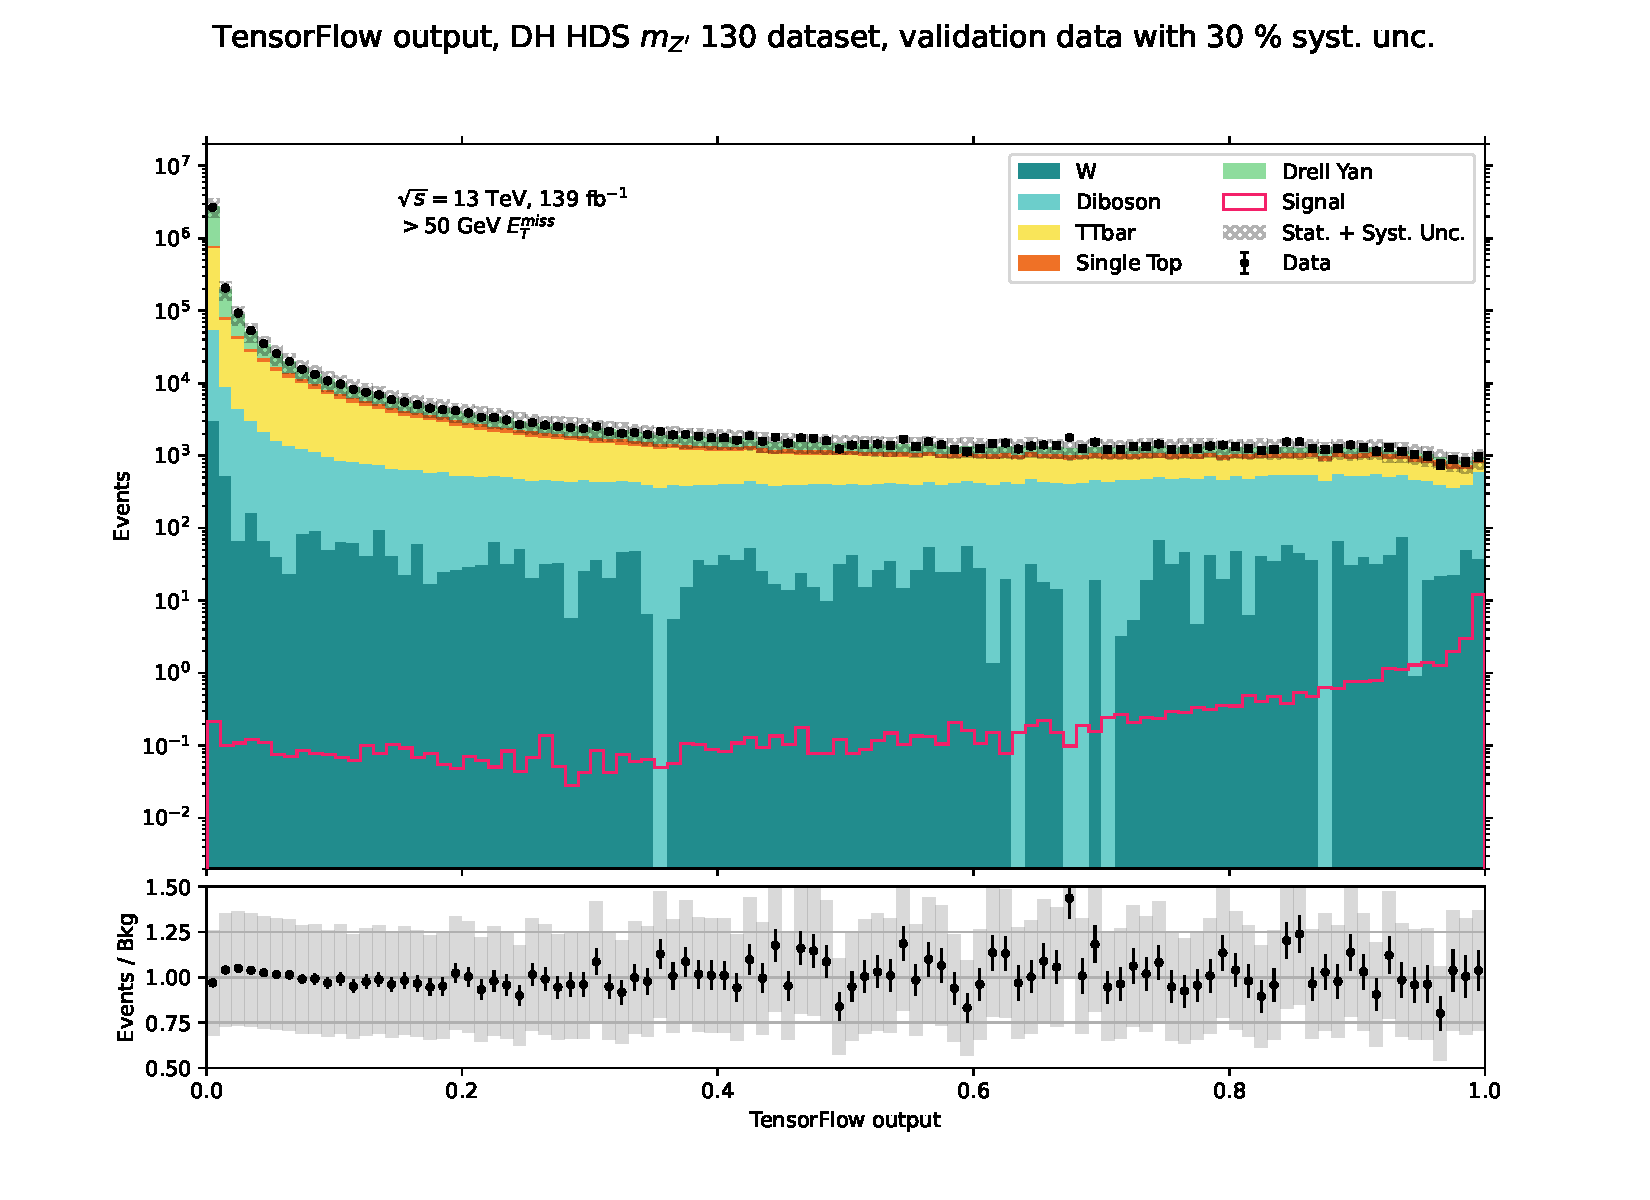
\includegraphics[width=1\textwidth]{new_variables/finer_binning/VAL.pdf}
      \caption{When including new variables and using 100 bins}
   \end{subfigure}
   \hfill
   \begin{subfigure}[b]{0.49\textwidth}
      \centering
      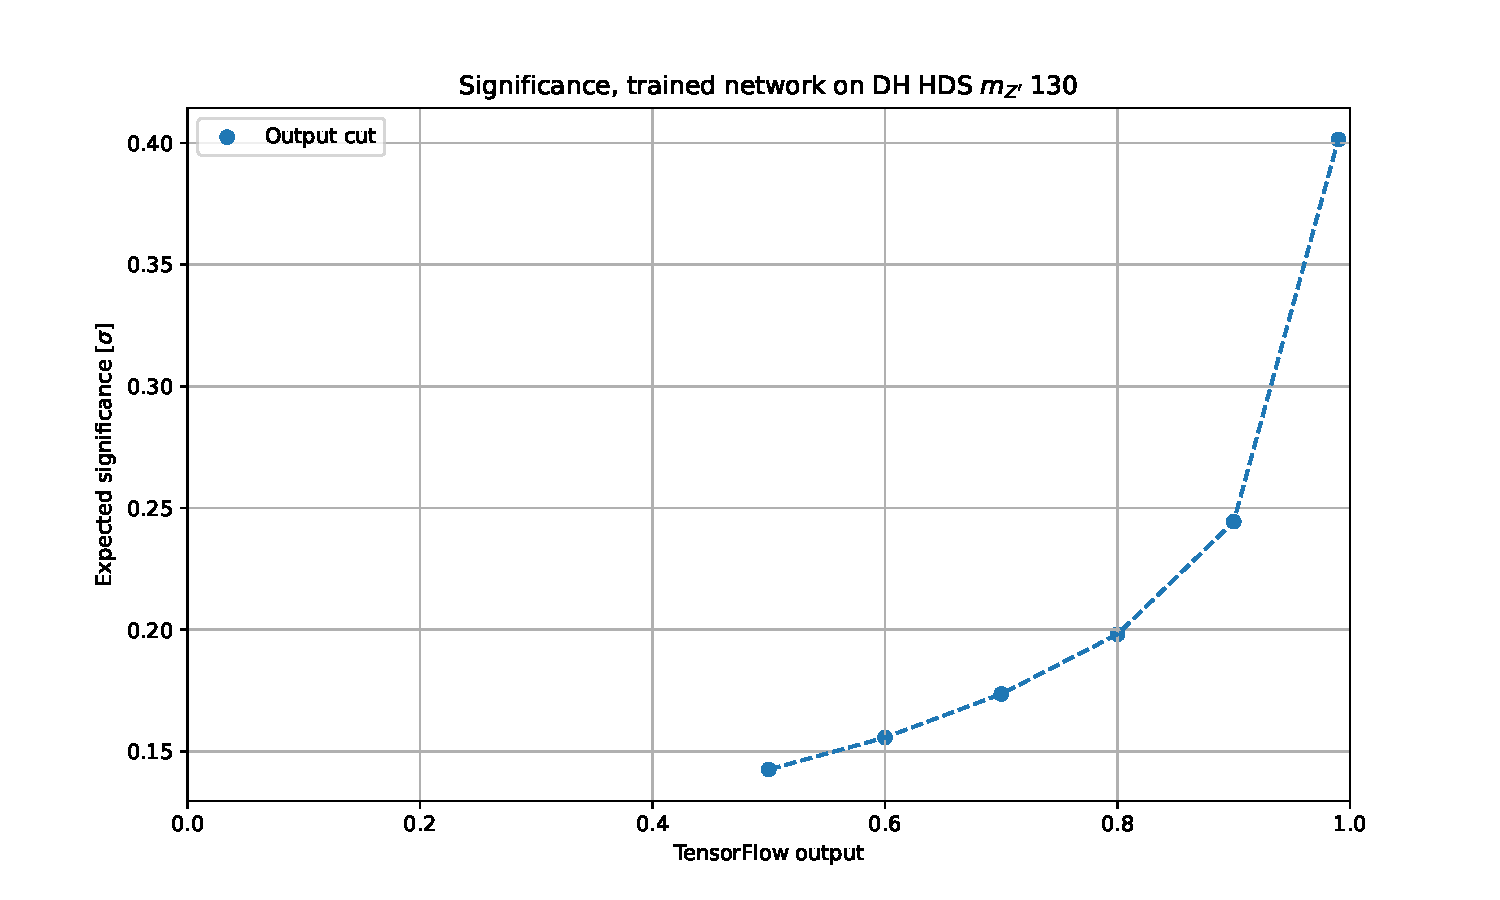
\includegraphics[width=1\textwidth]{new_variables/finer_binning/EXP_SIG.pdf}
      \caption{Expected significance of a)}
   \end{subfigure}
   \hfill
   \begin{subfigure}[b]{0.49\textwidth}
      \centering
      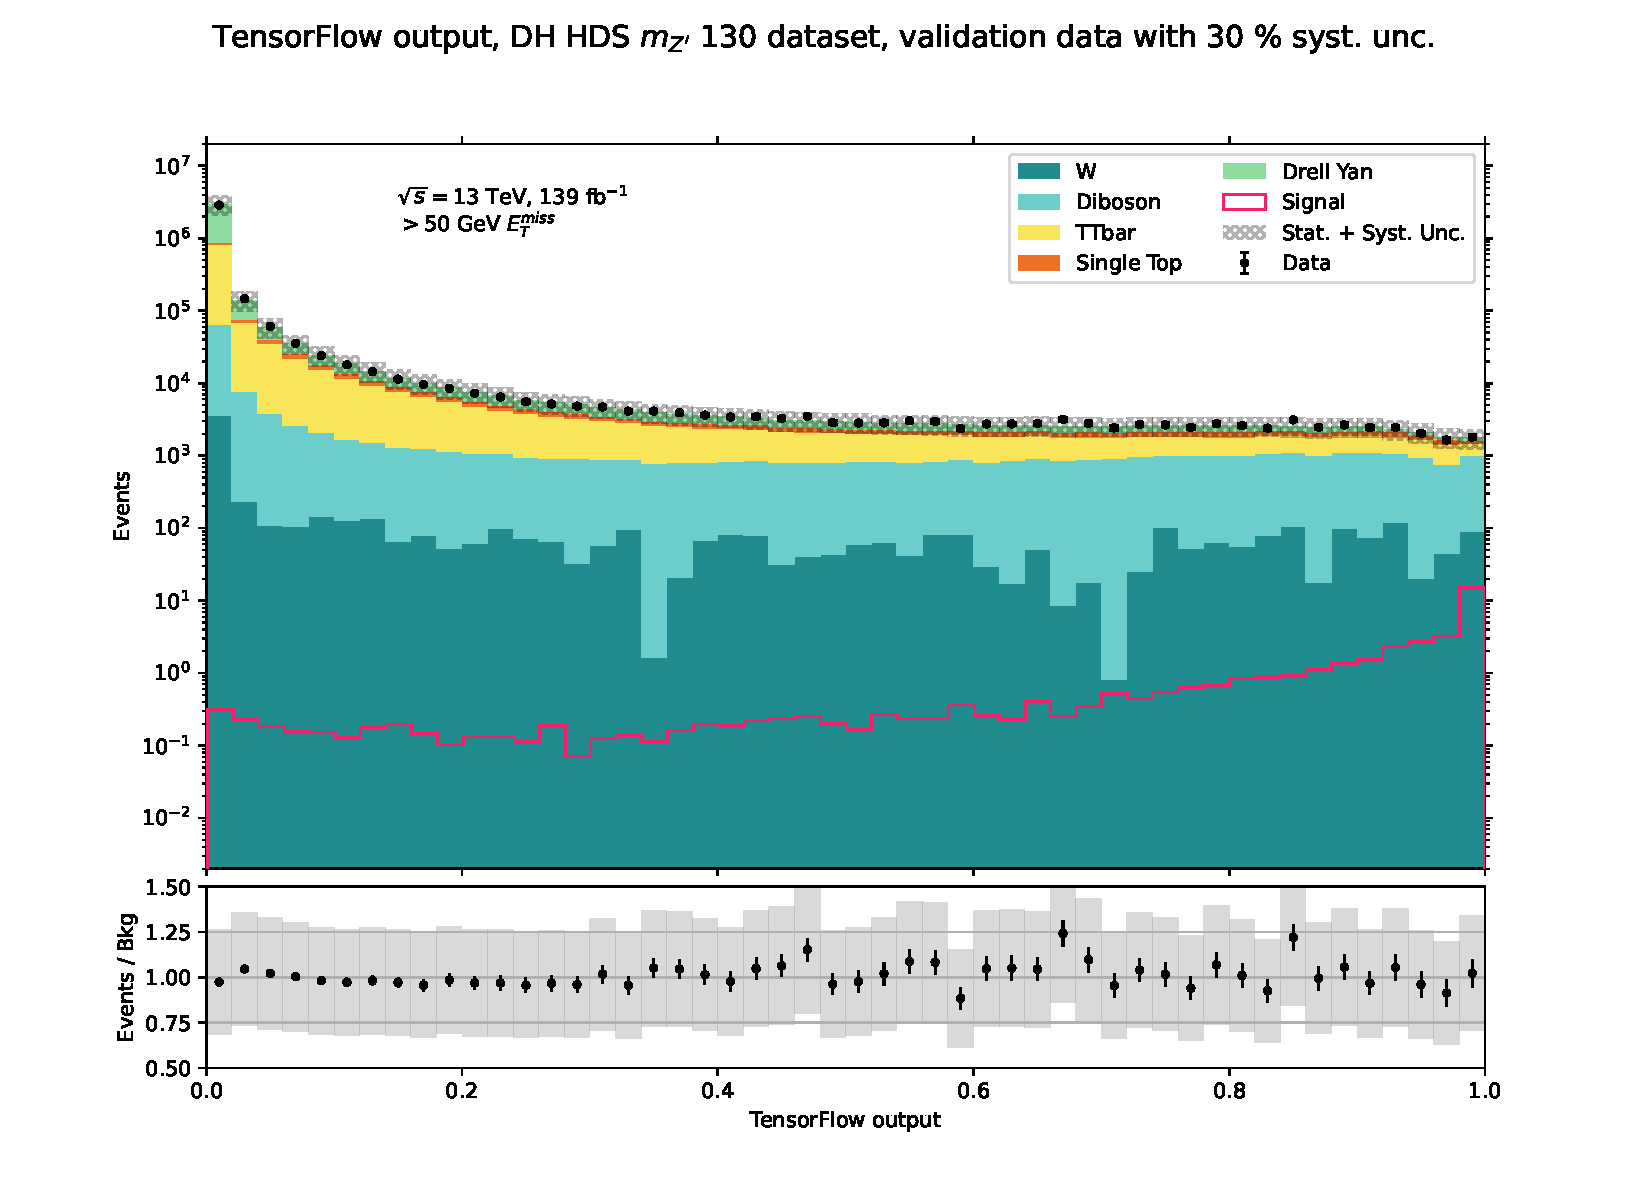
\includegraphics[width=1\textwidth]{new_variables/VAL.pdf}
      \caption{When including new variables and using 50 bins}
   \end{subfigure}
   \hfill
   \begin{subfigure}[b]{0.49\textwidth}
      \centering
      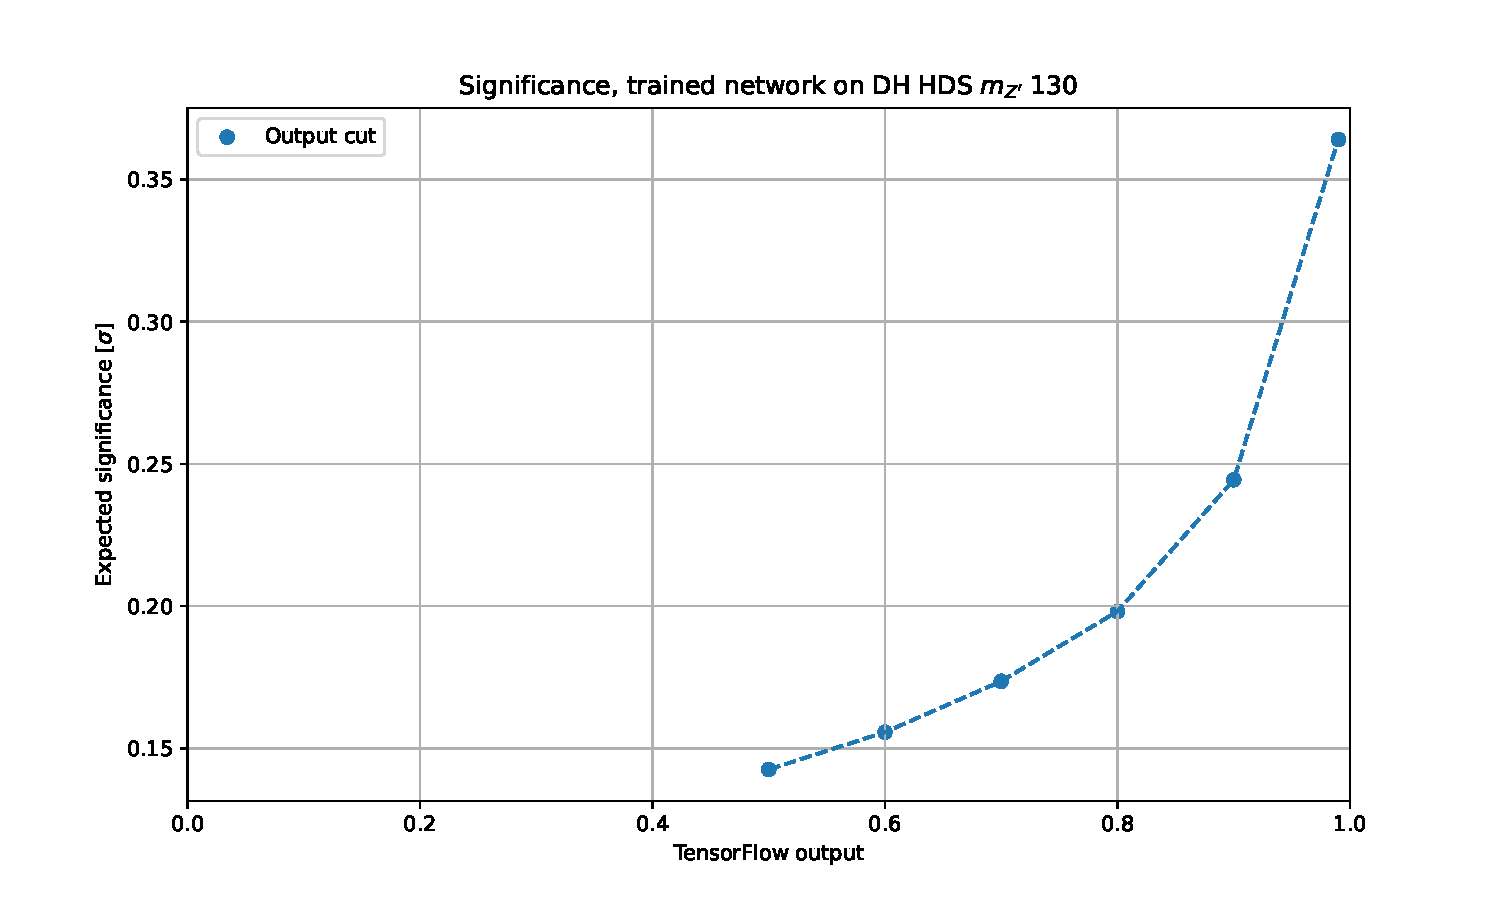
\includegraphics[width=1\textwidth]{new_variables/EXP_SIG.pdf}
      \caption{Expected significance of c)}
   \end{subfigure}
   \hfill
	\begin{subfigure}[b]{0.49\textwidth}
      \centering
      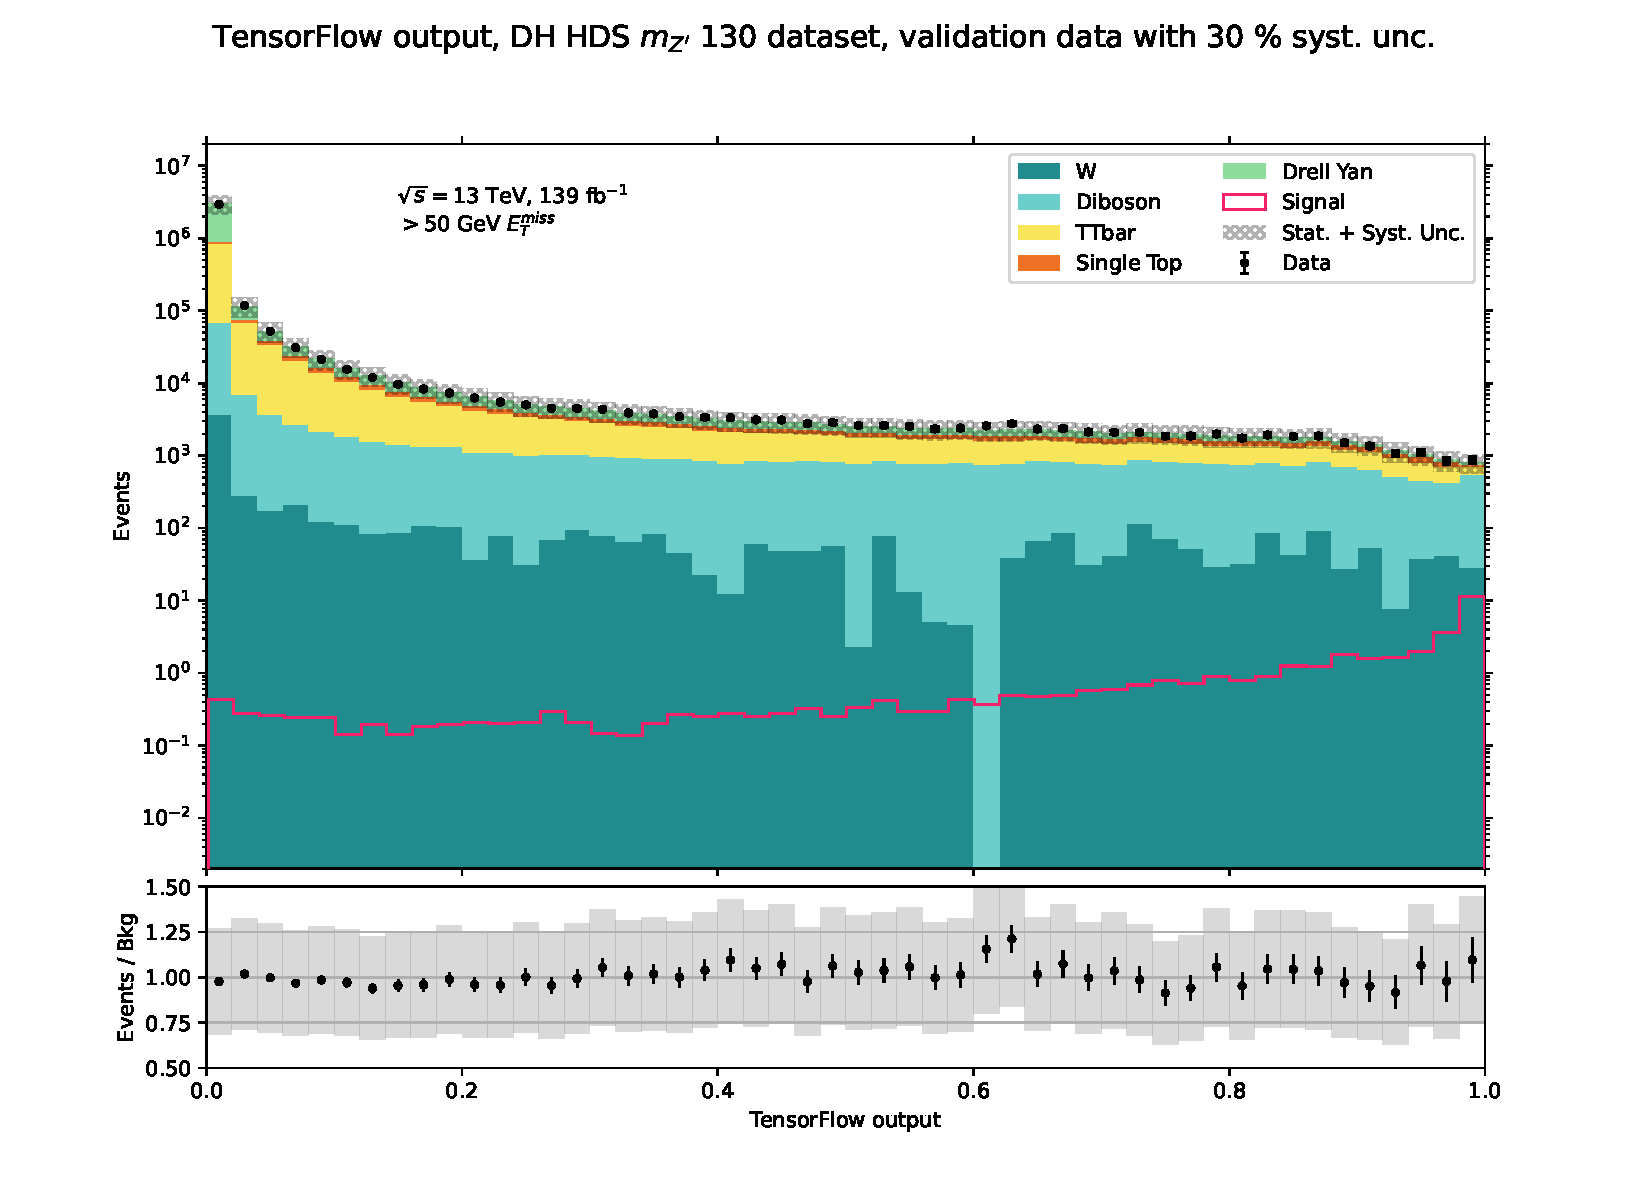
\includegraphics[width=1\textwidth]{no_pad/VAL.pdf}
      \caption{When excluding new variables and using 50 bins}
   \end{subfigure}
   \hfill
   \begin{subfigure}[b]{0.49\textwidth}
      \centering
      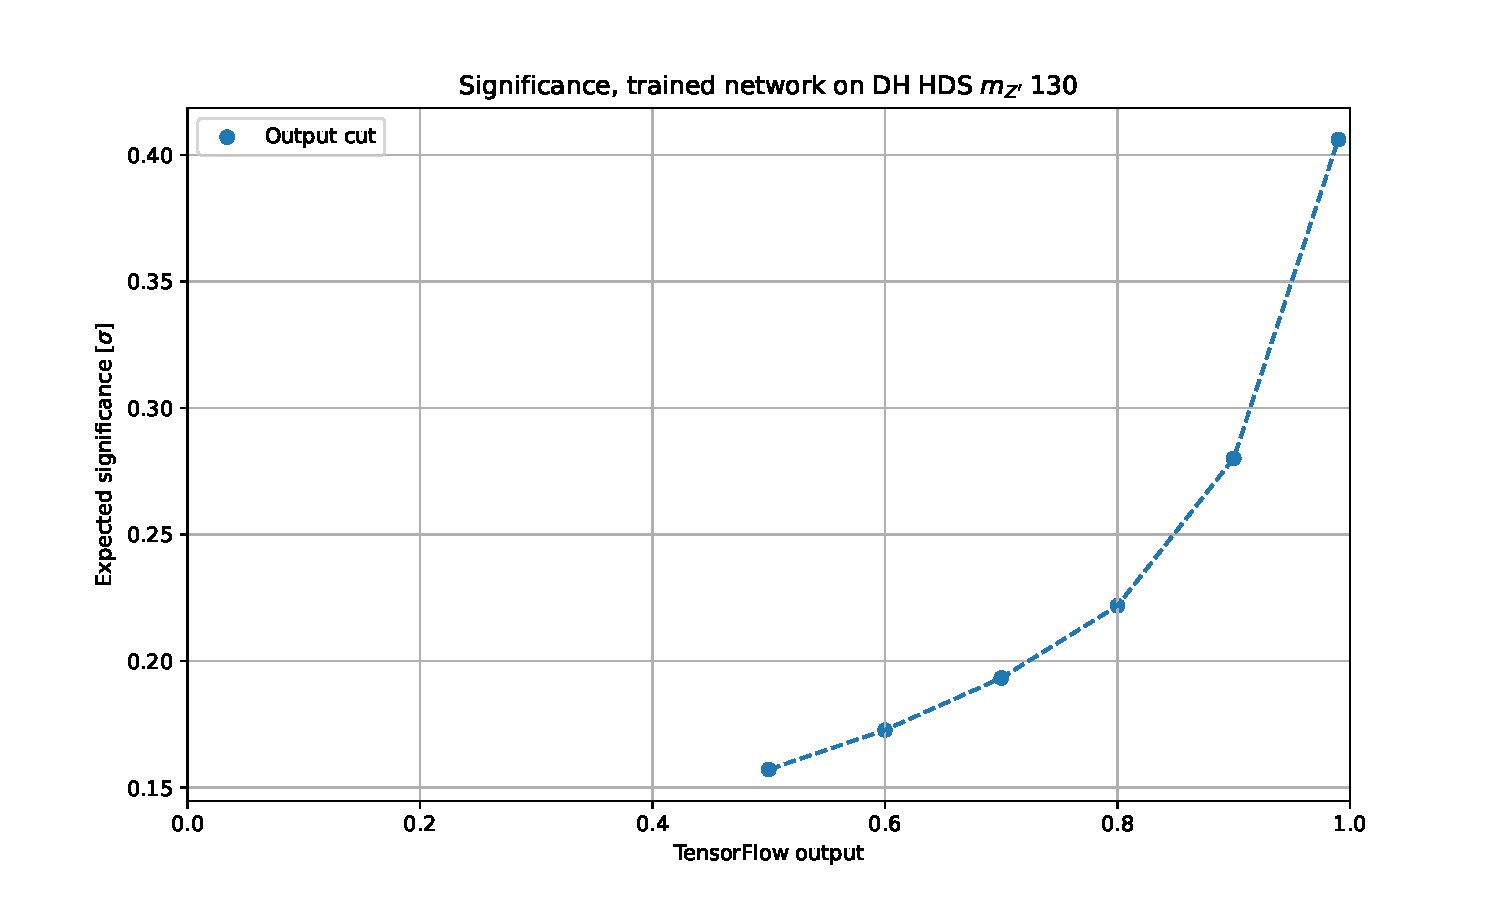
\includegraphics[width=1\textwidth]{no_pad/EXP_SIG.pdf}
      \caption{Expected significance of e)}
   \end{subfigure}
   \caption[Network performace when testing new variables to avoid padding]{NN prediction when using new features to avoid padding. This is testing a dataset with a Z' DM model.}\label{fig:New_var_pad}
\end{figure}
\clearpage


\subsection{Normalization of data}\label{sec:normie_NN}
Moving onto the second problem, which is not as problematic as the previous, we have the Normalization of data. Since neural networks send a lot of data into multiple neurons and mulitple layers using activation functions and other mathemathical tools, then it is important to make sure that the signal doesn't die when moving around the network. A fast way for the signal to die off is to not normalize the data and send it through the network, the reason it might die is because we send in numbers which vary significantly to eachother, i.e. the $p_{T}$ might be as high as thousands GeV, while $E_T^{miss}/\sigma$ might be as low as 0.1. What might happen when sending such different numbers is that the network might think "obviouly the high number is more important than the low number" thus making the activation function worse for the feature, even though this feature is of high imporatance when looking at MET final states.
A way to fix this problem is to normalize all features. There are many ways to do this, one could do \textit{min max scaling} which normalizes every feature from $[0,1]$, completely erasing the problem above. Mathematically speaking this is done by
\begin{equation}\label{eq:minmax}
   X_{norm} = \frac{X - X_{min}}{X_{max}-X_{min}}
\end{equation}
Where $X$ is the array containing all features, while $X_{min}$ and $X_{max}$ is the lowest and highest value in said array. Another way to normalize the data is to make the mean of the data 0 and the standard deviation to one, this is called \textit{Z-score normalization}
\begin{equation}\label{eq:Z-score}
   X_{norm} = \frac{X - \bar{X}}{\sqrt{\sigma_X^2}}
\end{equation}
where $\bar{X}$ is the mean of said array and $\sigma_X^2$ is the variance. One could also use pre-built functions in TensorFlow that do this normalization for you, one is called \verb|Batch_normalization| which normalizes the data that enters the network pr. batch, this is usually used in Convolutional NNs as it improves computational speed. 
And another one is simply \verb|Normalize| which does the same a Eq. (\ref{eq:Z-score}) for the whole training set going in, this is however computationally heavy to use. There is also \verb|Layer_normalization|, where you normalize the activations of the previous layer in a batch \textit{independently}, rather than \textit{across} a batch like \verb|Batch_Normalization|. But of these methods are also based on Z-score normaliazation. \\
\\There is a big difference when normalizing data ourselves and using TensorFlow, and that is that TensorFlow will remember how the data was normalized when training and will normalize the testing data in the same way (using the same variables), making testing easier.
These different normalization methods have been tested and can be seen in the Figure \ref{fig:DifferentNormalizations}. 
We can see that the best results come from Z-score and Batch normalization. We can see how the expected significance differs on both cases in Figure \ref{fig:BestNormie}.\\
\\From these results it is clear that the best normalization method is Batch normalization, but is it reasonable to use this method when one is not using a CNN? The reason batch normalization might work best for our case is because when we divide the data by bacthes it might unevenly represent the SM / signal and their ratio. But by using batch normalization it takes the average of all the batches creating an closer to real distribution. 
For the following examples in this section I have used the Z-score method, \todo{should I even mention this if I will not use NNs further?}but I will use Batch normaliazation for the signal search.\\ 
\graphicspath{{../../../Plots/TESTING/NeuralNetwork/NORMALIZATIONS/}}
\begin{figure}[!ht]
	\centering
	\begin{subfigure}[b]{0.49\textwidth}
      \centering
      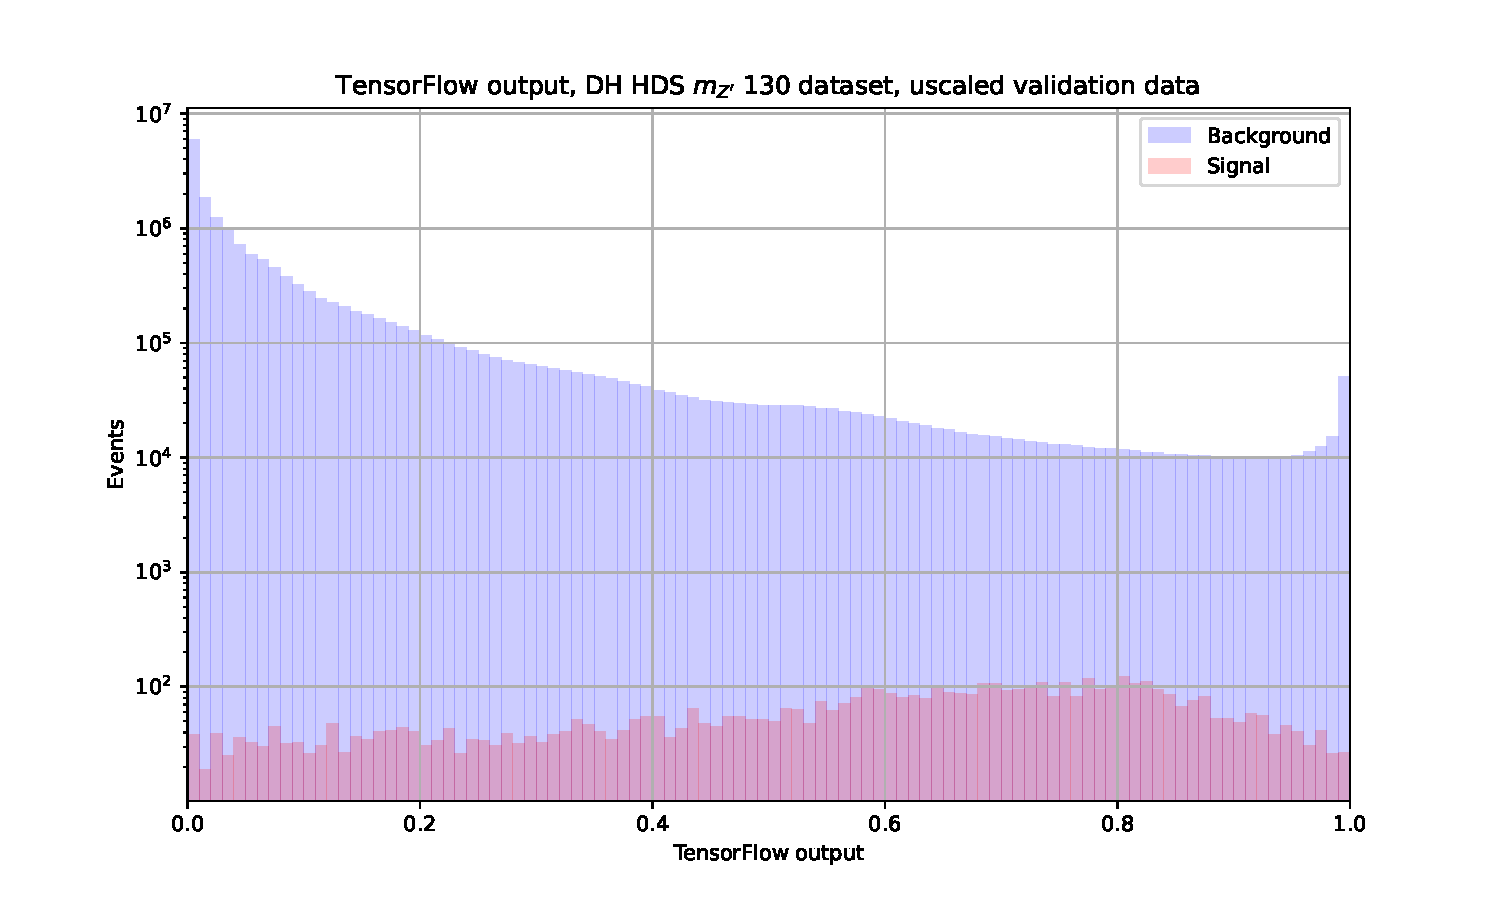
\includegraphics[width=1\textwidth]{NO_NORM/VAL_unscaled.pdf}
      \caption{No normalization}
   \end{subfigure}
   \hfill
   \begin{subfigure}[b]{0.49\textwidth}
      \centering
      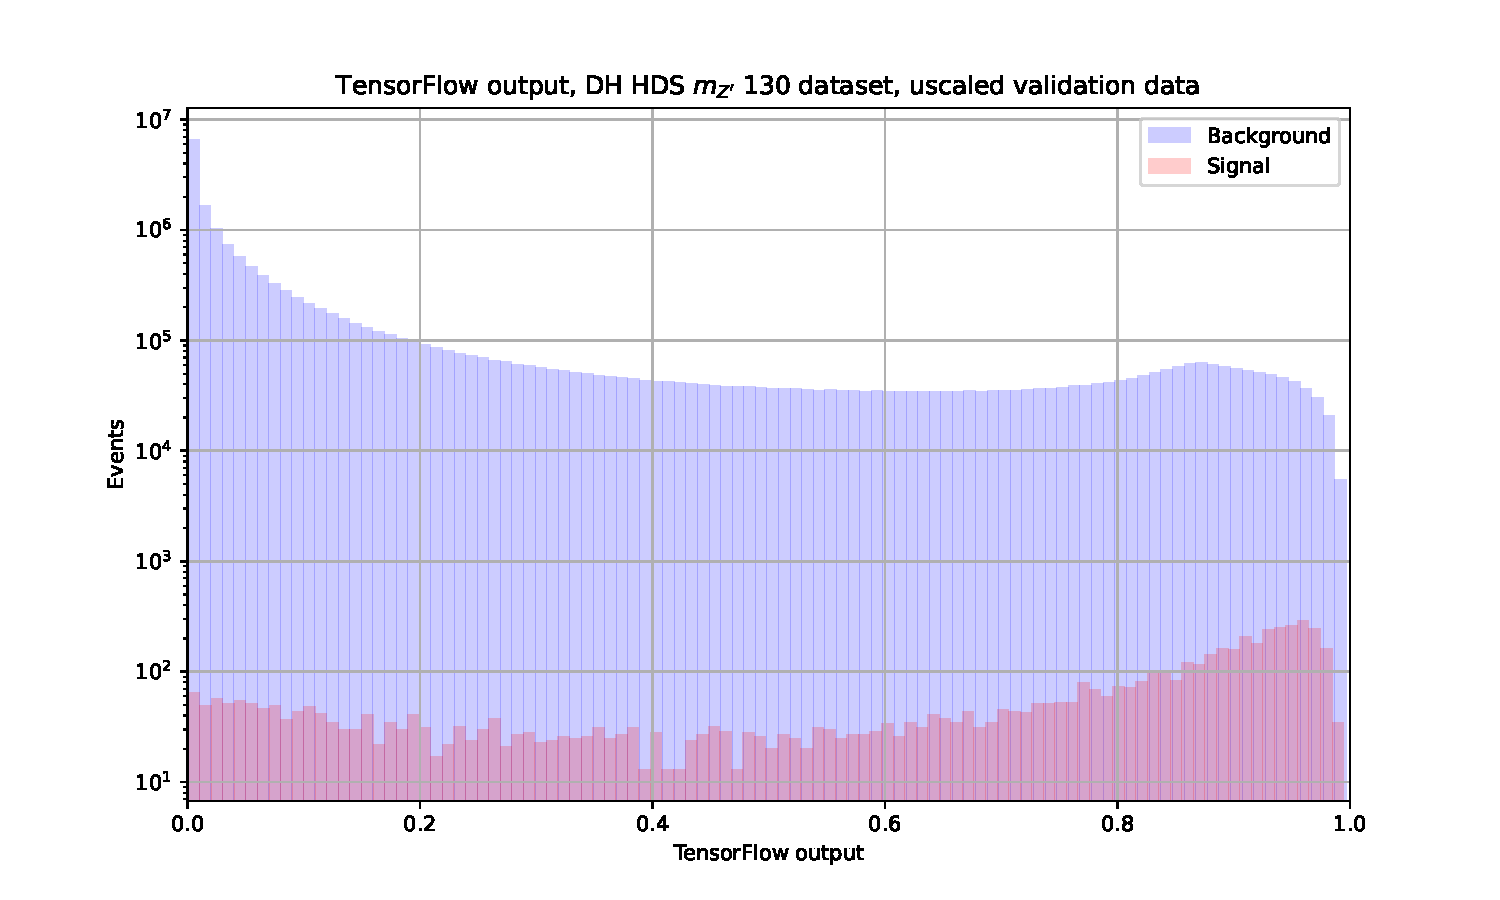
\includegraphics[width=1\textwidth]{Layer_norm/VAL_unscaled.pdf}
      \caption{Layer normalization}
   \end{subfigure}
   \hfill
	\begin{subfigure}[b]{0.49\textwidth}
      \centering
      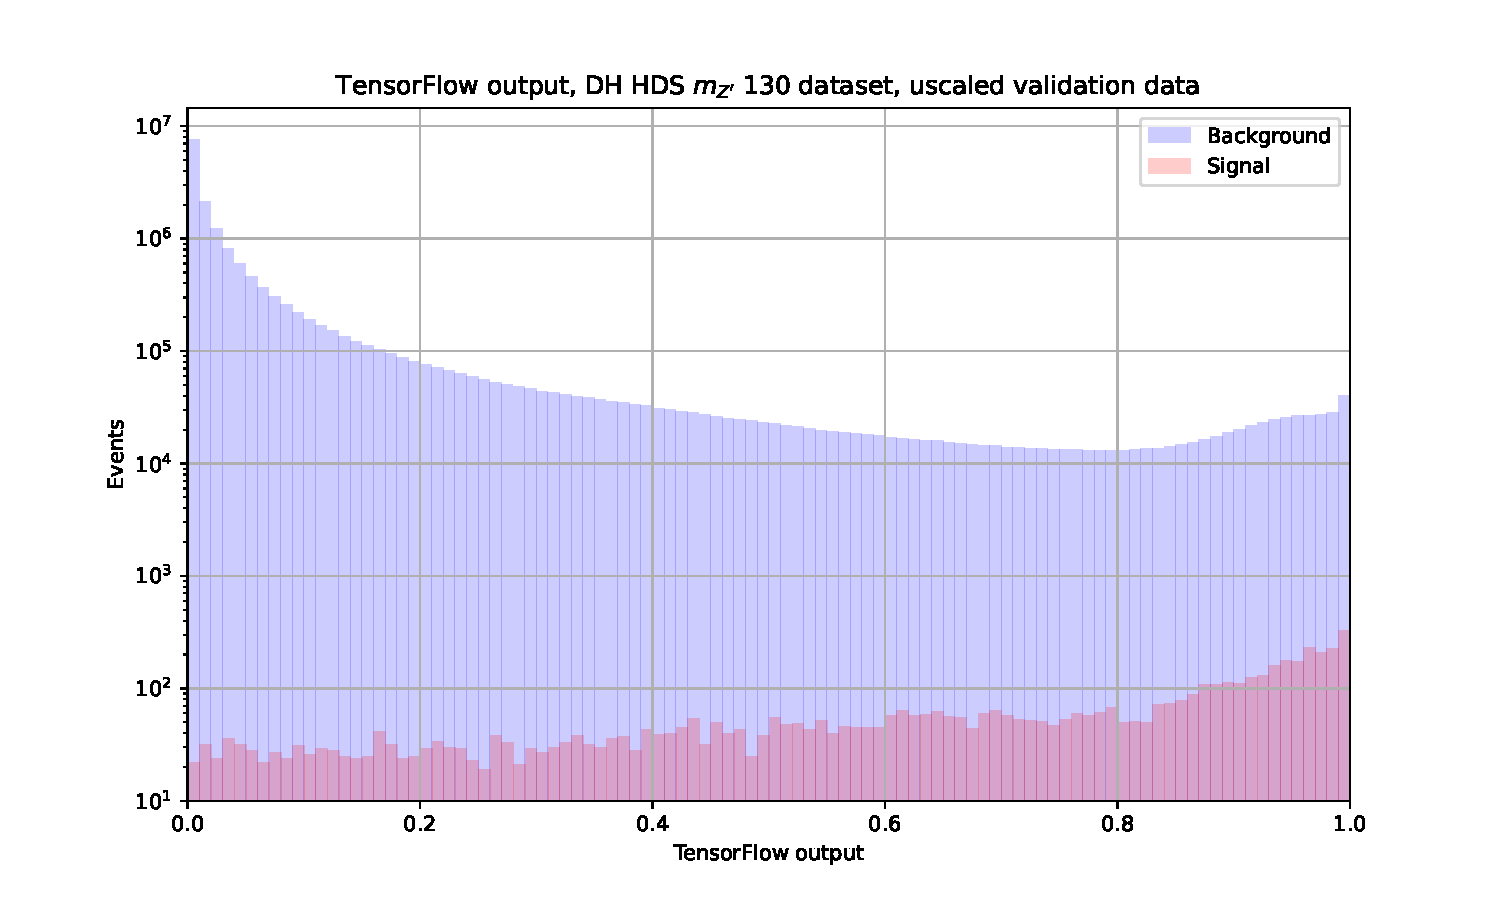
\includegraphics[width=1\textwidth]{minmax/VAL_unscaled.pdf}
      \caption{Min max scaling}
   \end{subfigure}
   \hfill
   \begin{subfigure}[b]{0.49\textwidth}
      \centering
      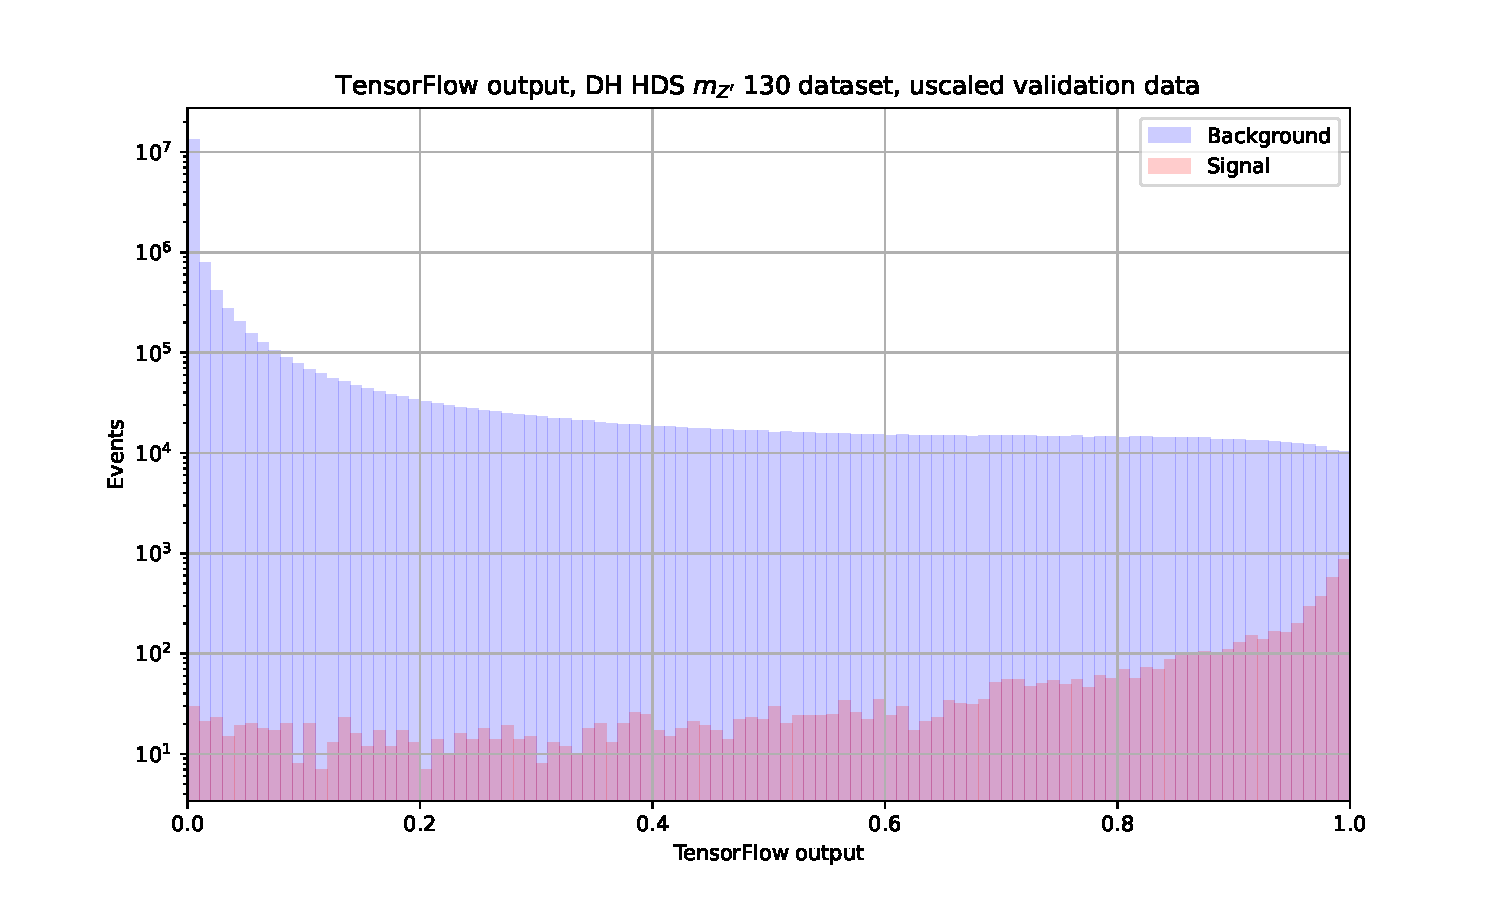
\includegraphics[width=1\textwidth]{Z_score/VAL_unscaled.pdf}
      \caption{Z-score}
   \end{subfigure}
   \hfill
   \begin{subfigure}[b]{0.49\textwidth}
      \centering
      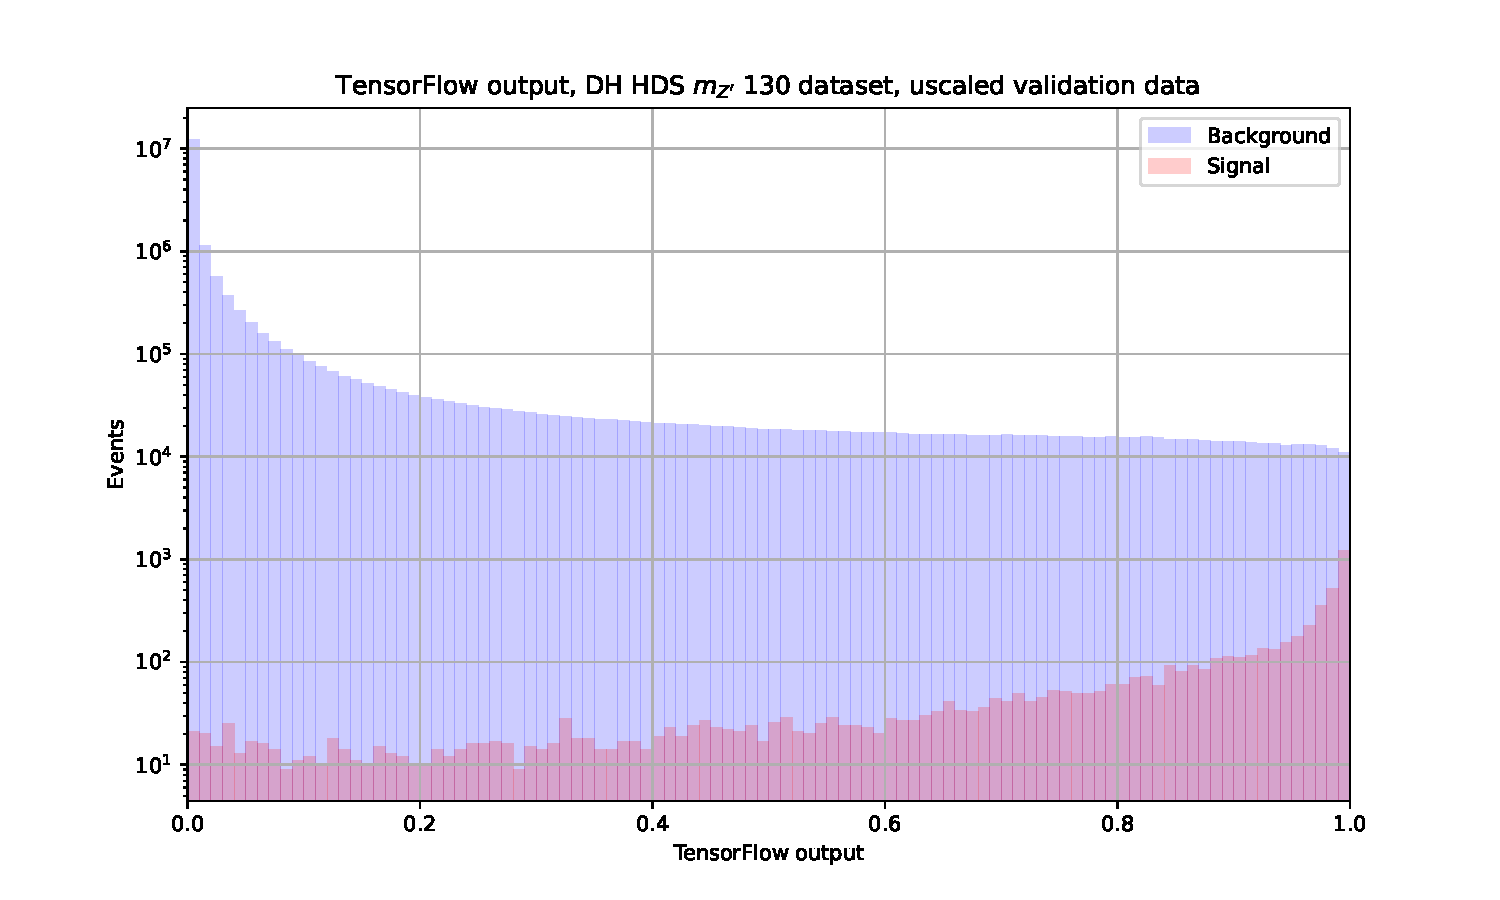
\includegraphics[width=1\textwidth]{Batch_norm/VAL_unscaled.pdf}
      \caption{Batch normalization}
   \end{subfigure}
   \caption{NN prediction when using different normalization methods. This is testing a dataset with a Z' DM model.}\label{fig:DifferentNormalizations}
\end{figure}


\begin{figure}[!ht]
	\centering
	\begin{subfigure}[b]{0.49\textwidth}
      \centering
      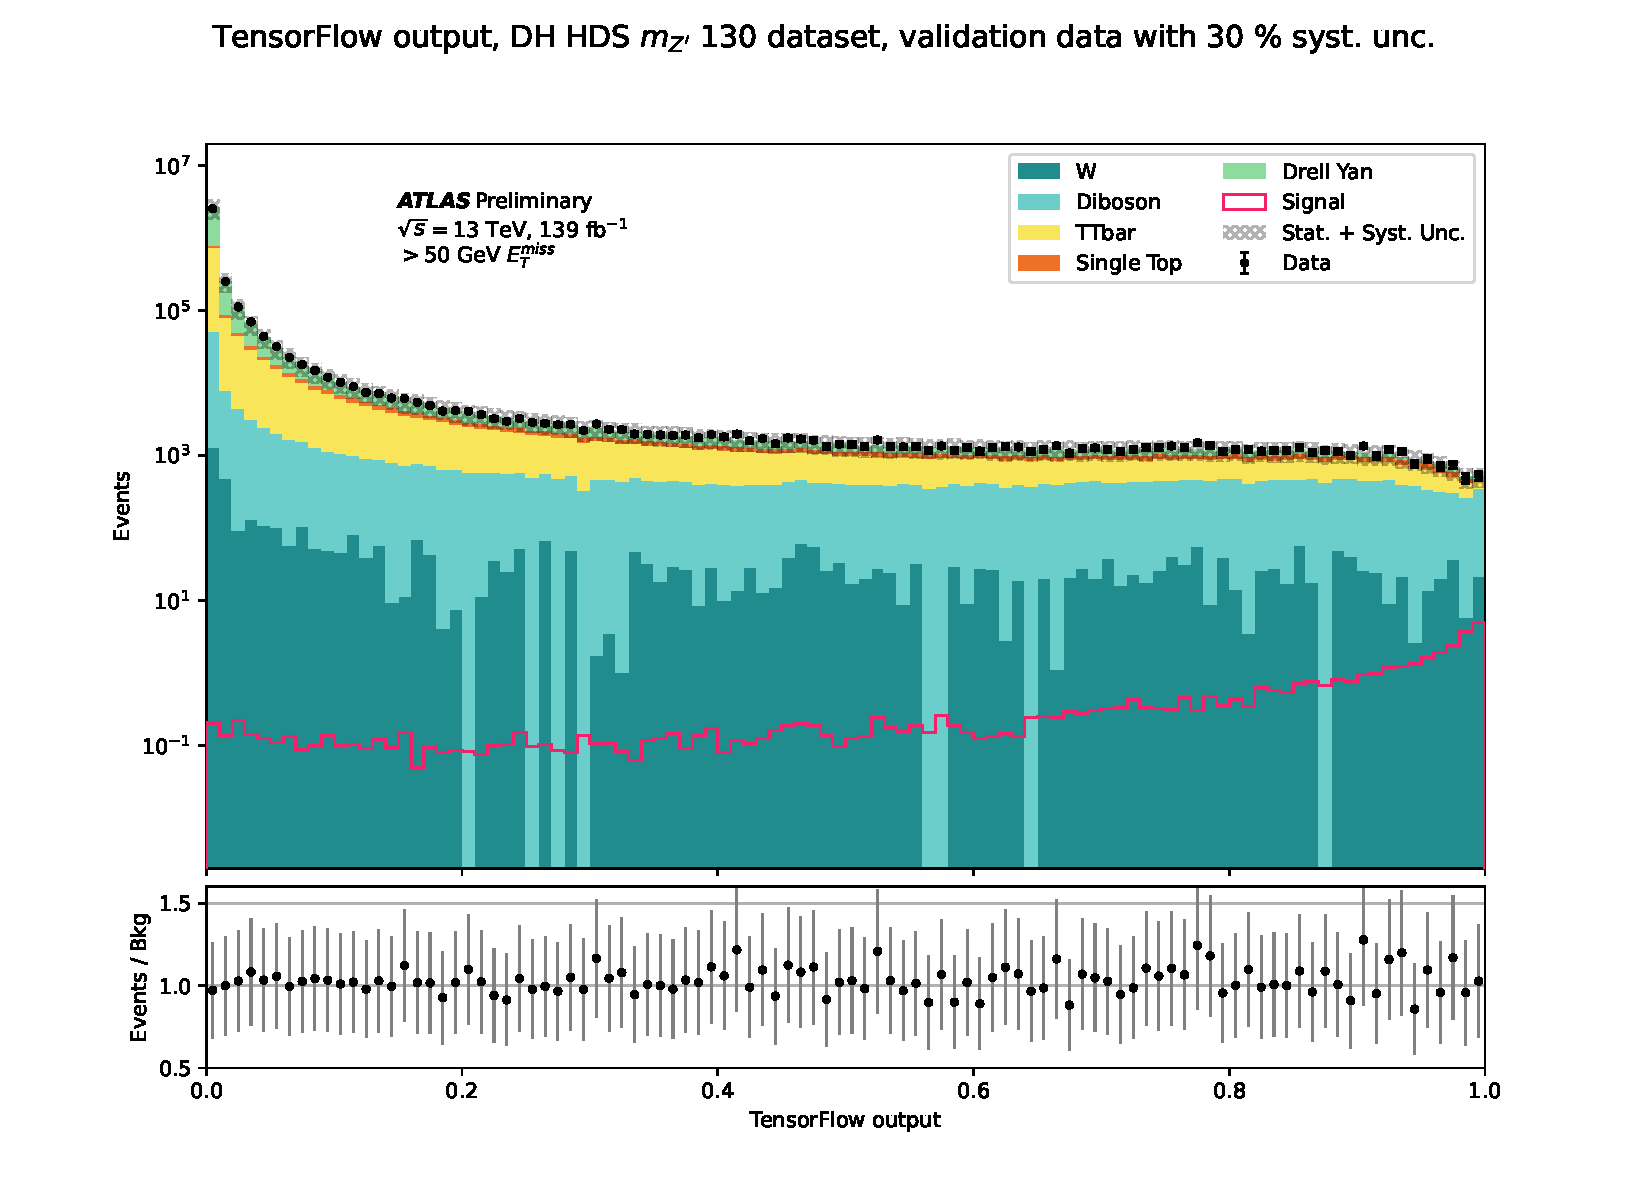
\includegraphics[width=1\textwidth]{Z_score/VAL.pdf}
      \caption{Z-score}
   \end{subfigure}
   \hfill
   \begin{subfigure}[b]{0.49\textwidth}
      \centering
      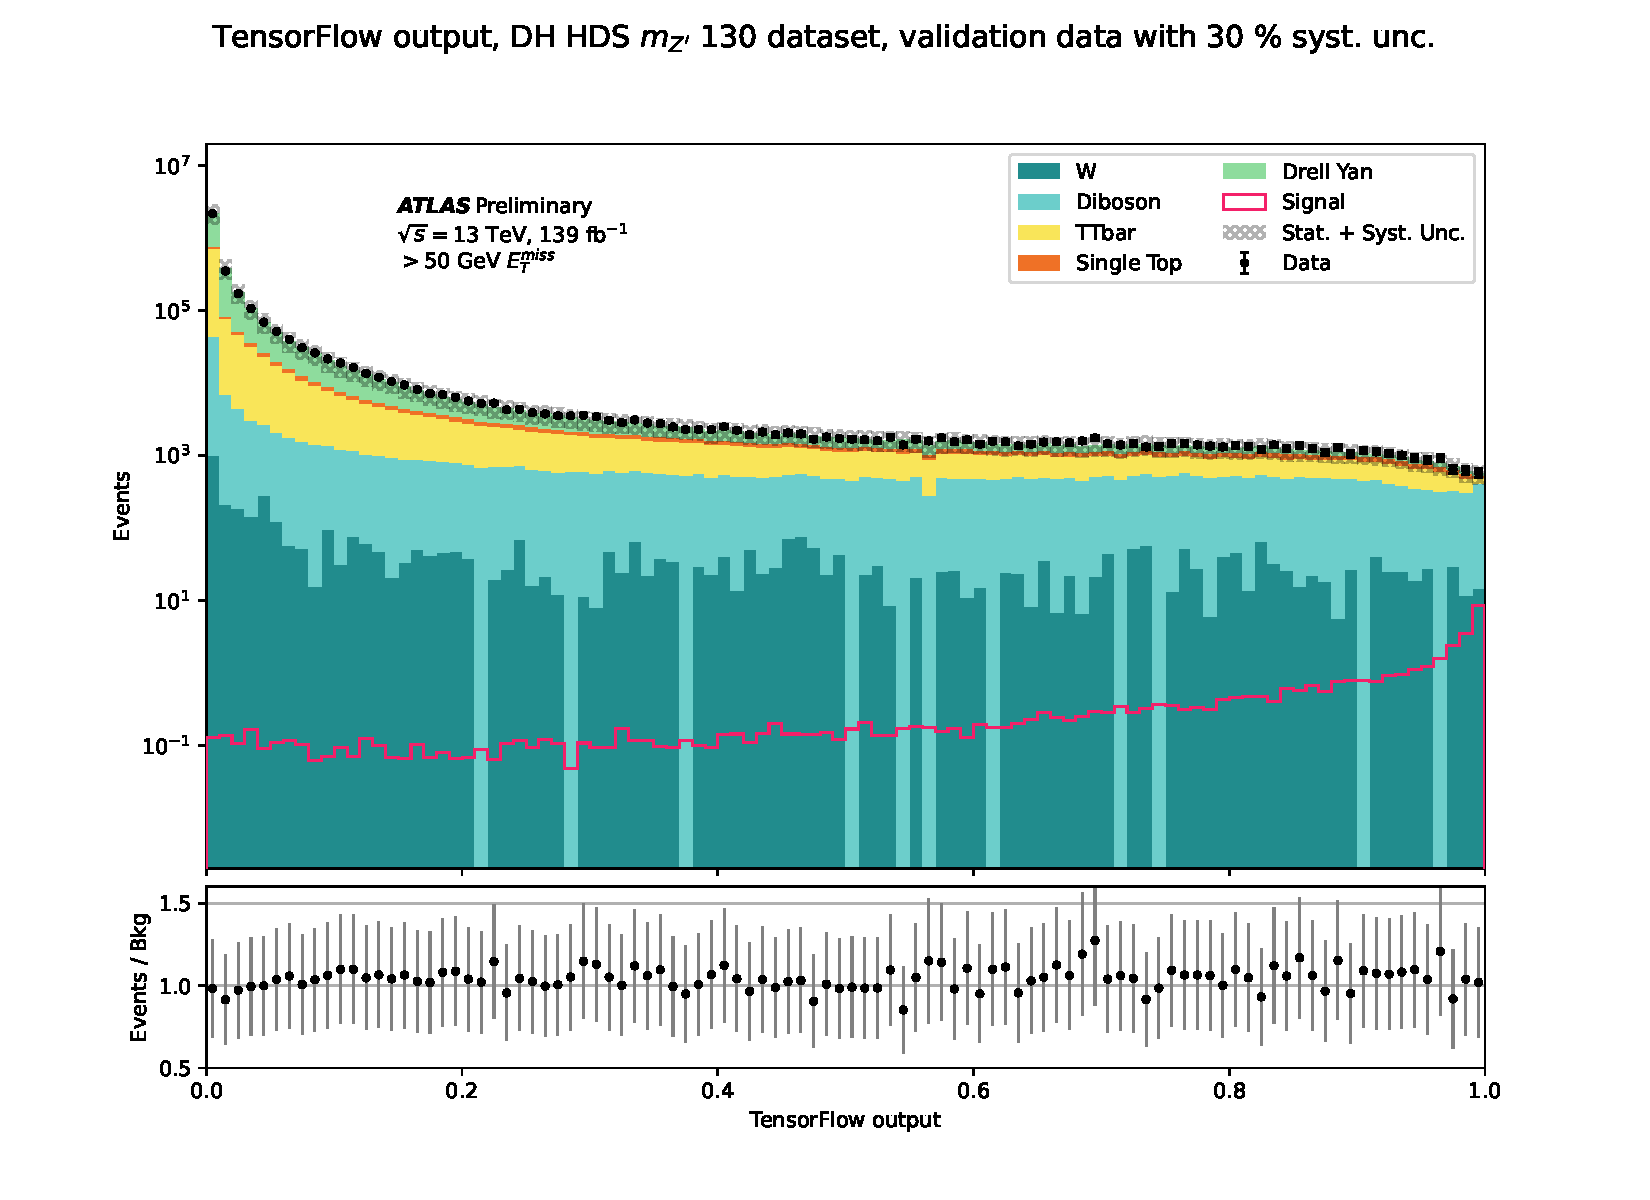
\includegraphics[width=1\textwidth]{Batch_norm/VAL.pdf}
      \caption{Batch normalization}
   \end{subfigure}
   \hfill
   \begin{subfigure}[b]{0.49\textwidth}
      \centering
      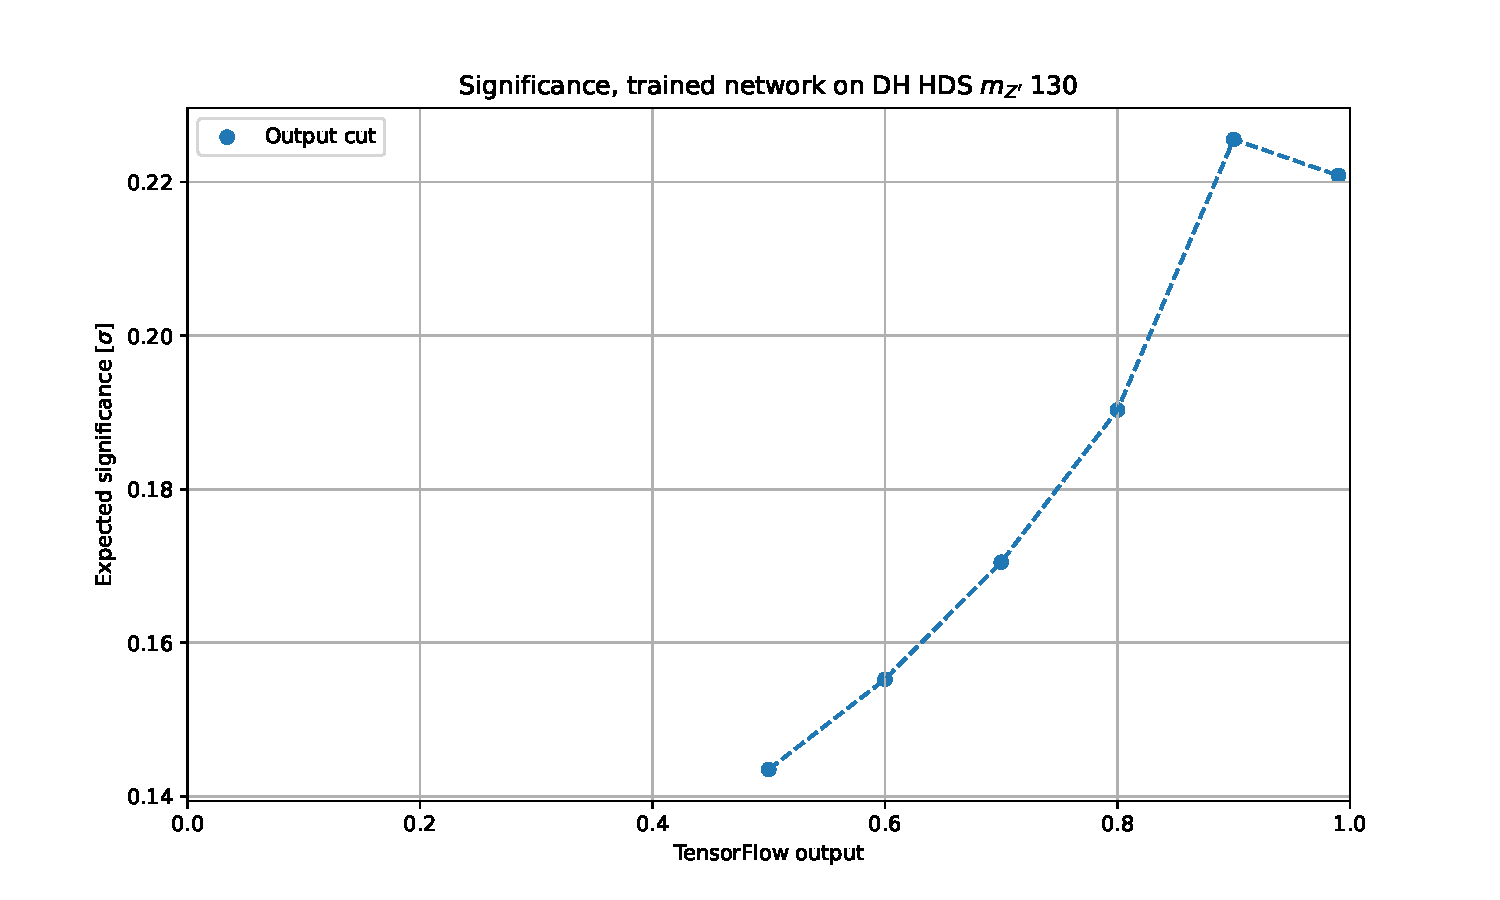
\includegraphics[width=1\textwidth]{Z_score/EXP_SIG.pdf}
      \caption{The expected significance of a)}
   \end{subfigure}
   \hfill
   \begin{subfigure}[b]{0.49\textwidth}
      \centering
      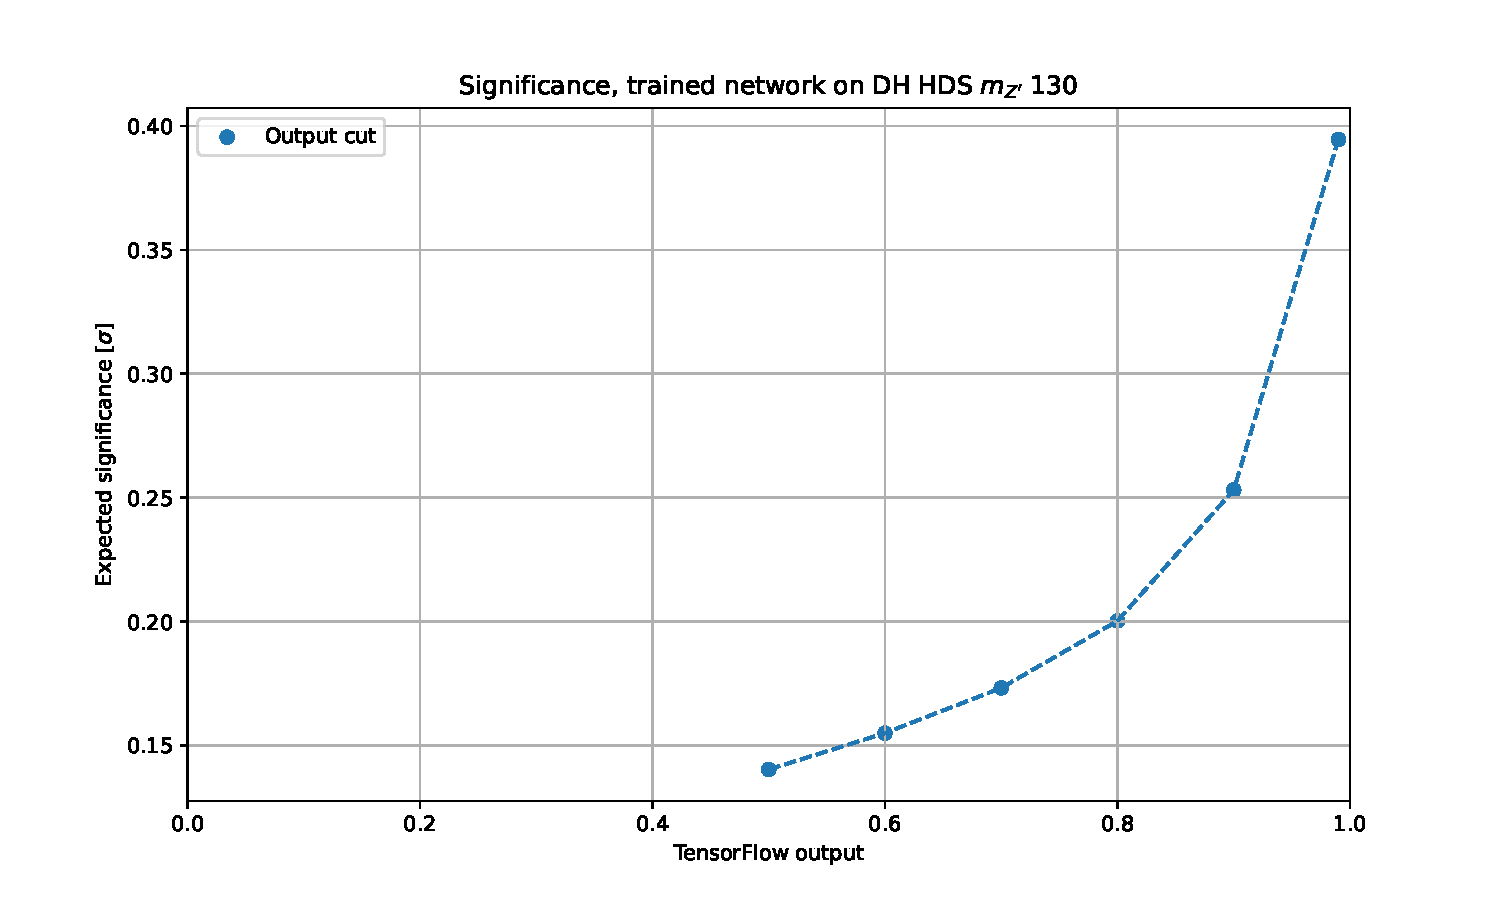
\includegraphics[width=1\textwidth]{Batch_norm/EXP_SIG.pdf}
      \caption{The expected significance of b)}
   \end{subfigure}
   \caption{Comparison of the best normalization methods. Figure a) and b) show the validation data of both cases, c) and d) show the expected significance of the validation plots when making a cut on the output. }\label{fig:BestNormie}
\end{figure}


\clearpage



\subsection{Weights}\label{sec:wgts}
\graphicspath{{../../figures/}}
A big problem that needs to be adressed in this thesis is what we should use as \textit{sample weights} (see Section \ref{sec:sample_weight}). If we were to not use any form of sample weights to mitigate the unbalance in our data set 
it could potentially lead to \todo{is it called undertraining?}undertraining where the networks could get "lazy" and guess that everything is background. If we were to split the full Z' data set into a training and test set, where 80\% is used for training, and trained a network without any weights then it seems as if the network excels in identifying our signal. 
This is however misleading as we need to keep in mind two things.\\
\\The first one, which \textbf{always} will be applied, is that we need to re-weight the MC events the networks trains on to the expected events, this we do by applying the weights explained in Setion \todo{will add this later!}... as well as factoring for the train-test split we made, 
that means that since our testing set is 20\% of the whole data set then we need to multiply this by 5 so we are back at 100\%. The difference is shown in Figure \ref{fig:OLD_FULL_DM_VAL}.\\ 
\begin{figure}[!ht]
	\centering
	\begin{subfigure}[b]{0.49\textwidth}
        \centering
        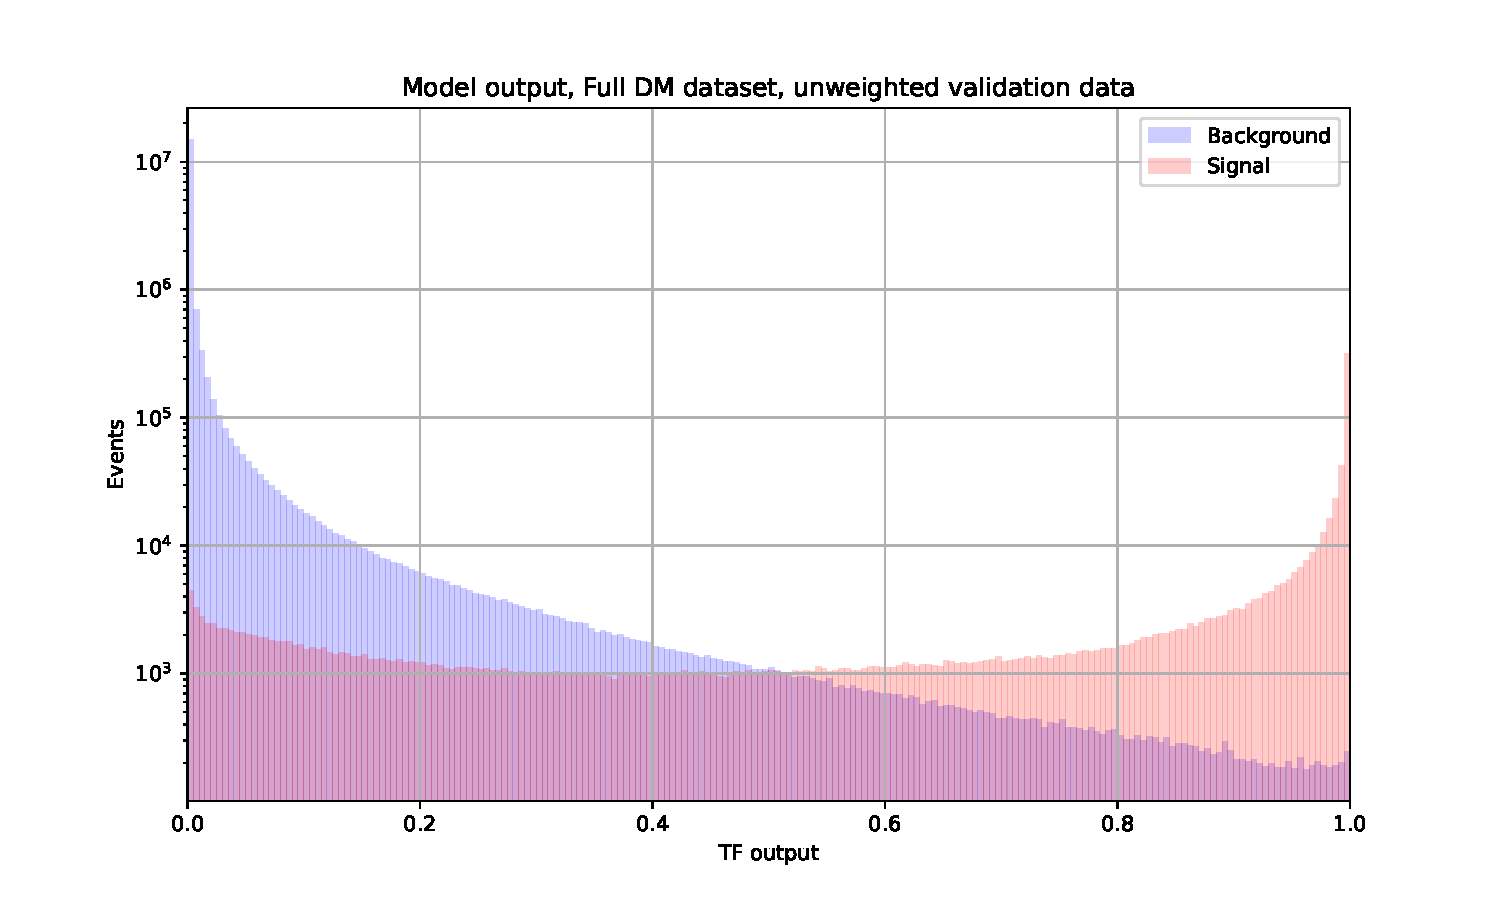
\includegraphics[width=1\textwidth]{OLD_DM_FULL_VAL_UNW.pdf}
        \caption{Unscaled validation plot.}\label{fig:OLD_UNW_FULL_DM_VAL}
     \end{subfigure}
     \hfill
     \begin{subfigure}[b]{0.49\textwidth}
        \centering
        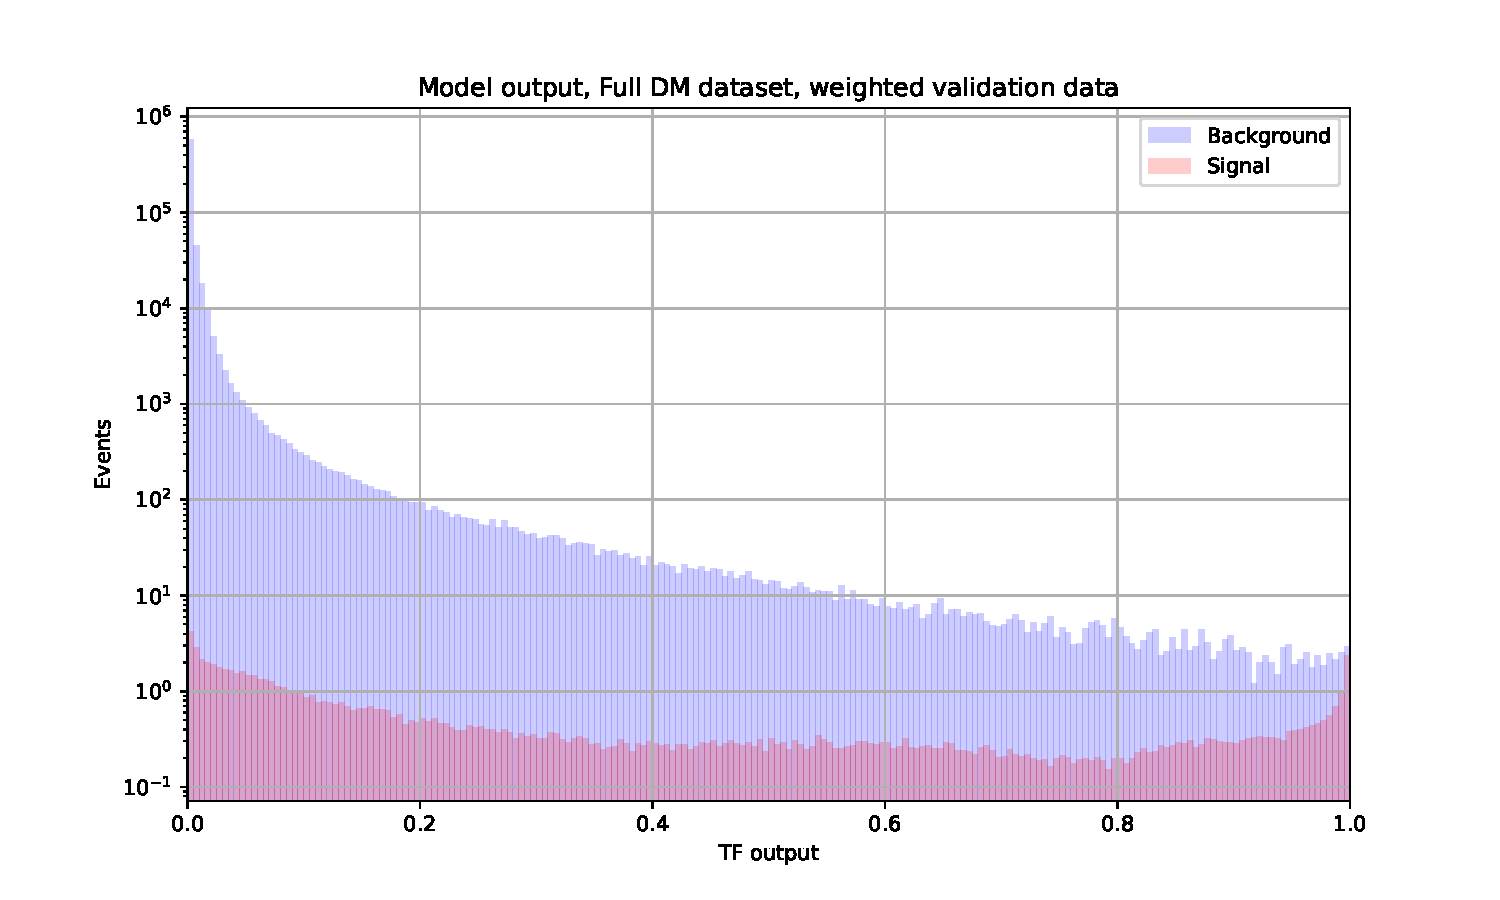
\includegraphics[width=1\textwidth]{OLD_DM_FULL_VAL_W.pdf}
        \caption{Scaled validation plot using MC weights.}\label{fig:OLD_W_FULL_DM_VAL}
     \end{subfigure}
	\caption[Importane of correctly scaling MC events to expected events]{Validation plot of uwweighted network on the first version of the FULL Z' DM dataset.}\label{fig:OLD_FULL_DM_VAL}
\end{figure}
\\The second thing, which is more important, is that we are not going to be testing our network on a "full data set", but rather on on one model with fixed parameters. For the purposes of most examples in this chapter, 
we will conduct our testing on one of the Z' models, more specially it will be a Dark Higgs (DH) with Heavy Dark Sector (HDS) and $m_{Z'}=130$ GeV. The reason I mention this here, and highlight its importance, is because 
the data imbalance \textbf{will} become a problem when we are studying just one specific model with fixed parameters. To put some numbers, the whole SM background we are studying has roughly 87 million MC events, 
the whole Z' signal has roughly 3 million MC events, and the DH HDS $m_{Z'} = 130$ GeV model has 40,000 MC events! So if the network were to say that every event is a background event when testing on the small model with fixed parameters, 
it would be correct over 99.9\% of the time. This is obviously something we do not want, as our goal is to make a ML algorithm that actually learns DM signatures.\\
\\I trained a network to find the Diboson background channel among the other SM backgrounds to find a general solution to what weights will be used to balance using the sample weight feature, as this is something we know exists. 
The imbalance of this data set can be seen in Table \ref{tab:UnbalancedDibosonTraining}.
\begin{table}[!h]
   \centering
   \begin{tabular}{l|r|r|r}\midrule\midrule
                   & Number of MC events  & Number of expected events   & MC events $\times$ expected events [$10^{11}$]\\\midrule
        Signal     & 8,813,716            & 93,304.9                    & 8.2\\
        Background & 61,201,010           & 2,621,498.9                 & 1,604.4 \\ \midrule\midrule
   \end{tabular}
   \caption[Unbalanced Diboson training dataset]{Table Showcasing how uneven the training dataset is between signal and background. This is on the Diboson dataset which incorporates all the SM MC samples}
   \label{tab:UnbalancedDibosonTraining}
\end{table}
\\The reason for this choice and not a DM signal, is because I \todo{should I write this or skip it entirely?}wrongly assumed when first testing the network, that the network \textit{correctly} predicted that there were no DM events. 
Put in rougher words, I thought that the network completely dismissed the model by claiming it did not exist, and thus excluding the whole model, a very bold, pretentious and wrong claim. 
As my first attempt to use weights used the same weights used to re-weight MC events to expected events, which included the cross section of every event... this will become important later.\\
\\As expected, my interpretation was wrong, the network trained using the weights to re-weight MC events on the Diboson search also predicted that there were "0 Diboson events", something we can empirically and confidently say is wrong. 
Moreover, the validation plot of the unweighted network works, but gives poor results. As a method to balance the signal and background, I made a new weight array to be used as sample weight. This array weights down all background events 
with the ratio of MC signal events over MC background events, $\frac{N_{sig}}{N_{bkg}}$. The results are shown in Figure \ref{fig:DibosonVAL} and the ROC scores in Figure \ref{fig:DibosonROC}.\\
\begin{figure}[!ht]
	\centering
	\begin{subfigure}[b]{0.49\textwidth}
        \centering
        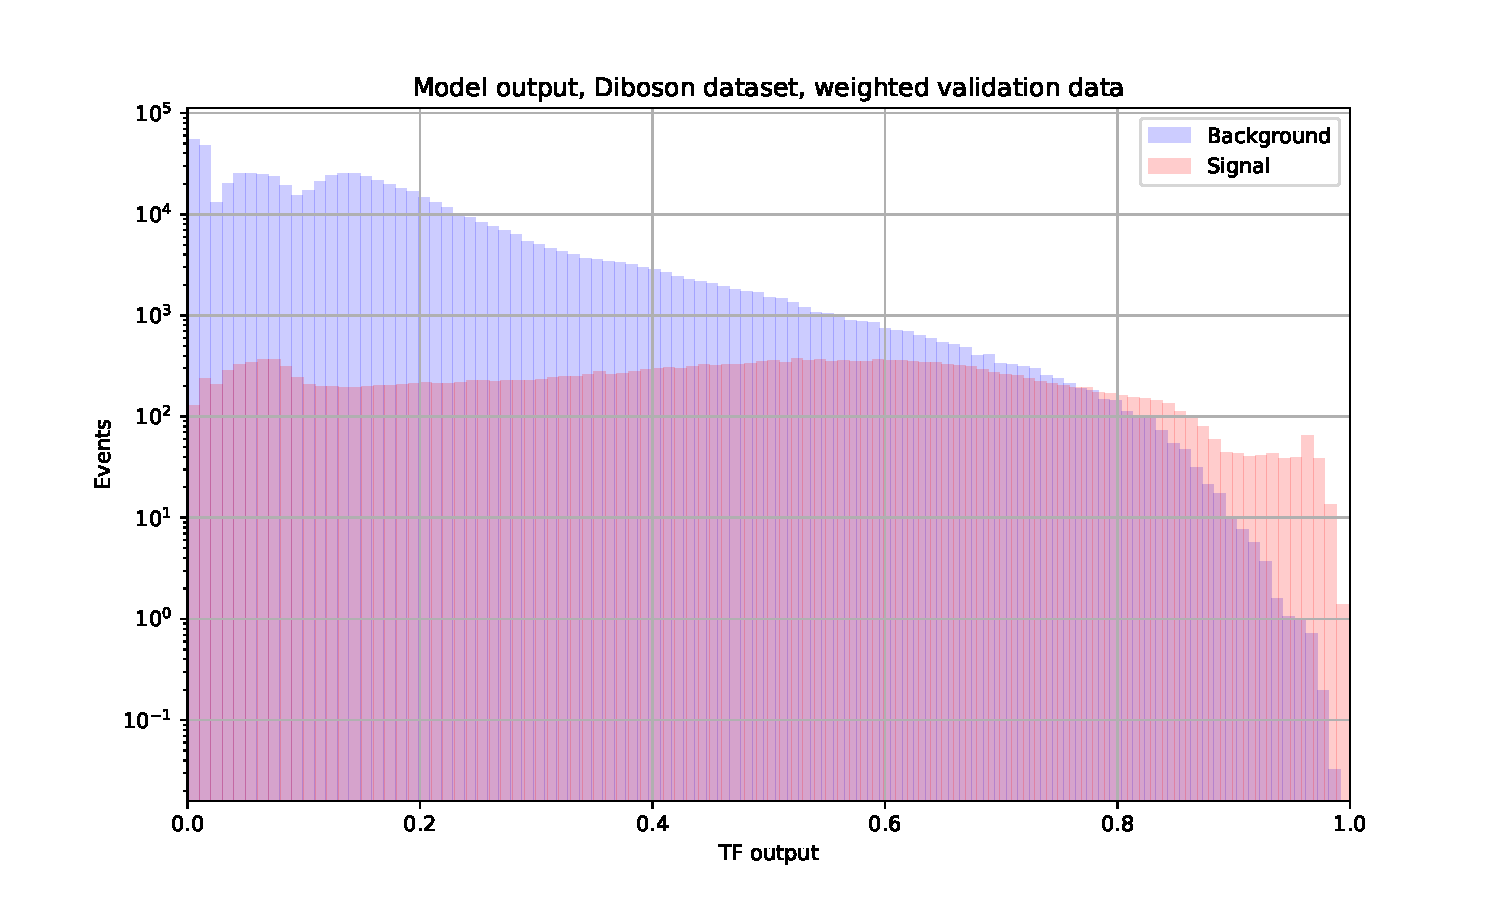
\includegraphics[width=1\textwidth]{VAL_uw.pdf}
        \caption{Validation plot for the unweighted training.}\label{fig:DibosonVALUW}
     \end{subfigure}
     \hfill
     \begin{subfigure}[b]{0.49\textwidth}
        \centering
        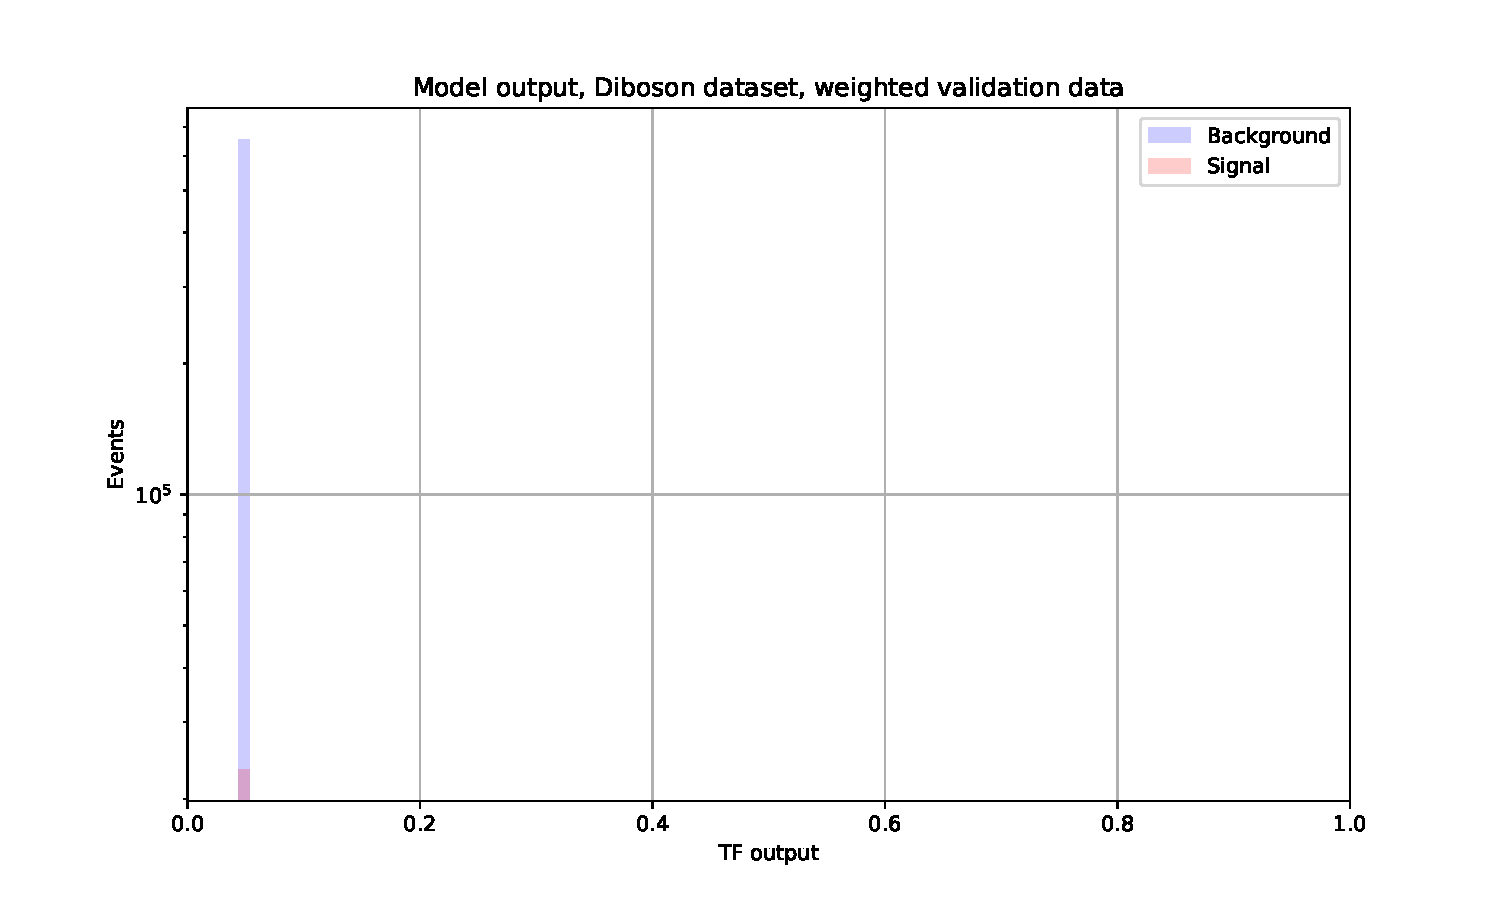
\includegraphics[width=1\textwidth]{VAL_mc.pdf}
        \caption{Validation plot for the weighted training using MC weights.}\label{fig:DibosonVALMC}
     \end{subfigure}
     \begin{subfigure}[b]{0.49\textwidth}
        \centering
        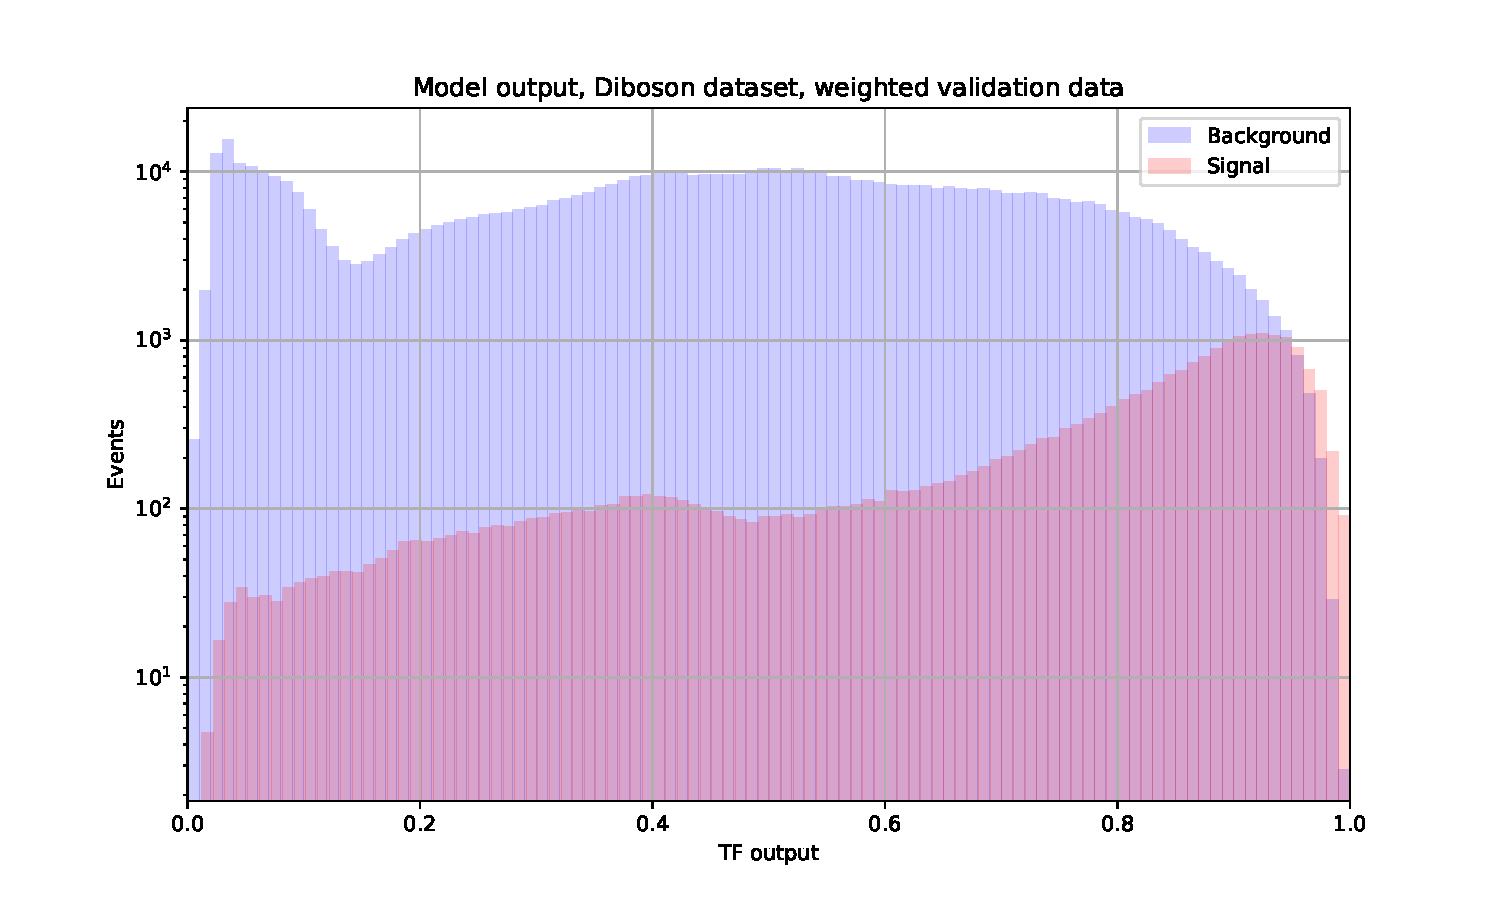
\includegraphics[width=1\textwidth]{VAL_w.pdf}
        \caption{Validation plot for the weighted training using $\frac{N_{sig}}{N_{bkg}}$ as weights on the background.}\label{fig:DibosonVALW}
     \end{subfigure}
	\caption{Result of the different network training weighting.}\label{fig:DibosonVAL}
\end{figure}
\begin{figure}[!ht]
	\centering
	\begin{subfigure}[b]{0.49\textwidth}
        \centering
        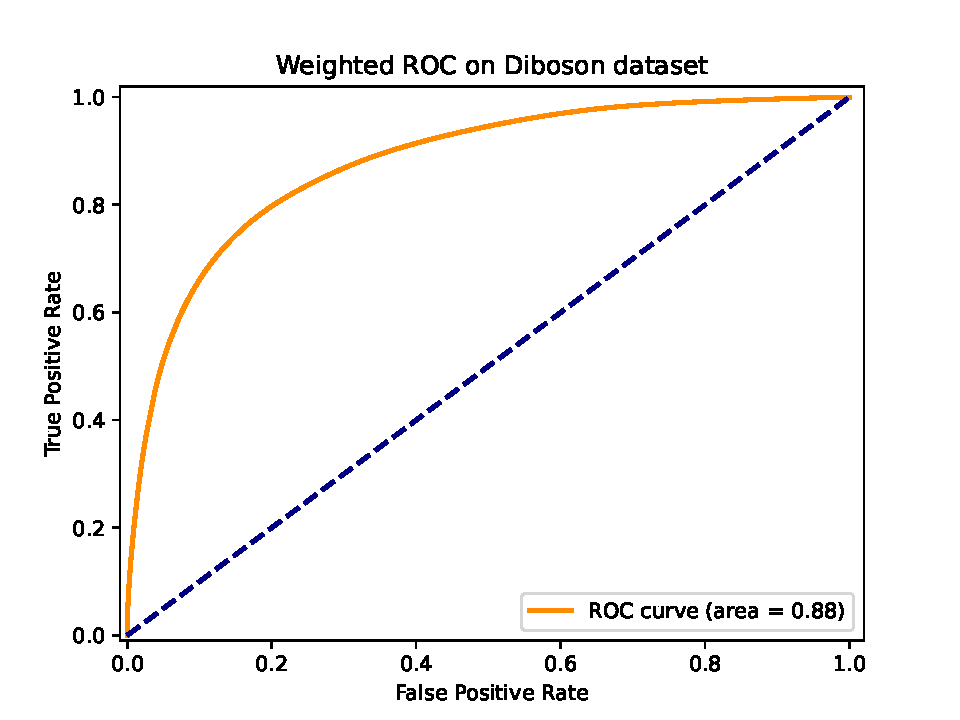
\includegraphics[width=1\textwidth]{ROC_uw.pdf}
        \caption{ROC score for the unweighted training.}\label{fig:DibosonROCUW}
     \end{subfigure}
     \hfill
     \begin{subfigure}[b]{0.49\textwidth}
        \centering
        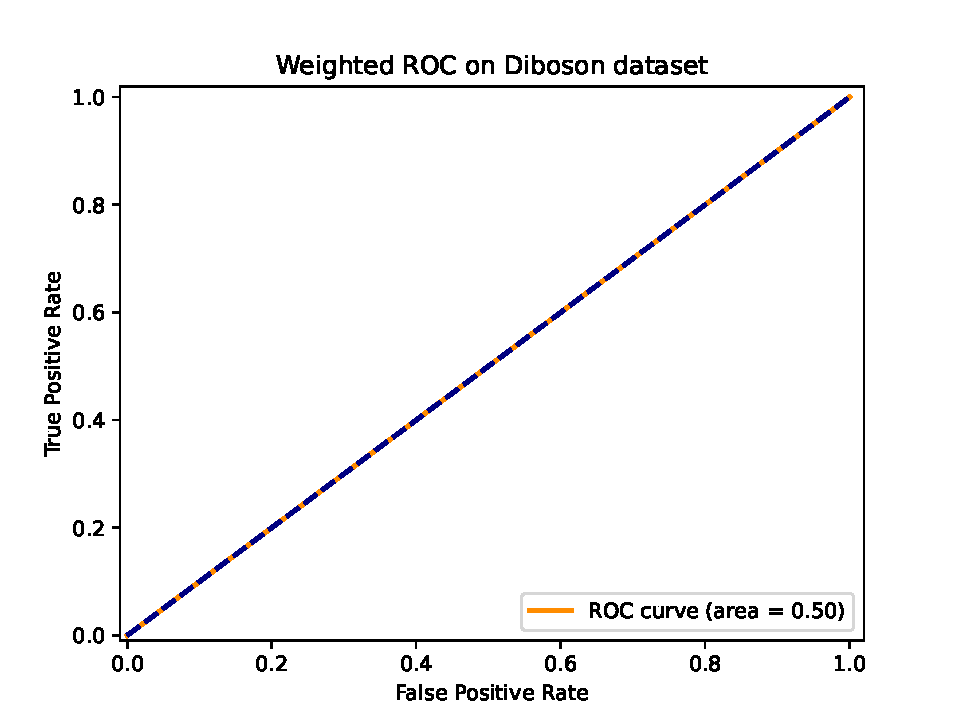
\includegraphics[width=1\textwidth]{ROC_mc.pdf}
        \caption{ROC score for the weighted training using MC weights.}\label{fig:DibosonROCMC}
     \end{subfigure}
     \begin{subfigure}[b]{0.49\textwidth}
        \centering
        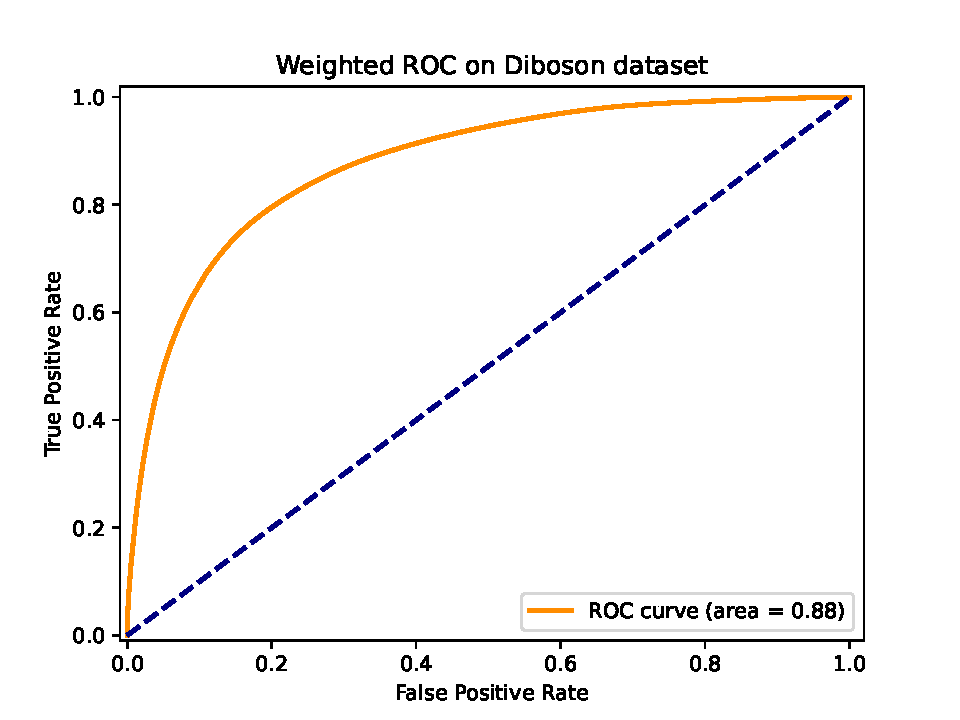
\includegraphics[width=1\textwidth]{ROC_w.pdf}
        \caption{ROC score for the weighted training using $\frac{N_{sig}}{N_{bkg}}$ as weights on the background.}\label{fig:DibosonROCW}
     \end{subfigure}
	\caption{Result of the different network training weighting.}\label{fig:DibosonROC}
\end{figure}
\\From the results we see that the new weighting method has a poorer result than the unweighted one, and the weighting method that re-weight MC events to expected events just crashes the whole network. 
The reason for why the latter does not work might be since the network gets punished by guessing "too easily" that an event is signal, and instead of trying harder to learn the patterns and predict with "more confidence" 
signal events just guesses that everything is a background event and still get a high \textit{accuracy}\footnote{Not to be confused with AUC!}. Something else to mention, as to why the network does such a poor job at classifying the diboson background, is that the network here was not optimized for the search, and rather just used the 
defaul NN settings on TensorFlow. \todo{mention this or remove completely}And to make matters worse, when testing this I had a bug where I used zero hidden layers by accident, meaning that there was in fact no NN.


\clearpage



\subsection{Balanced weights\todo{This whole section is my reasoning for trying to re-weight the MC events to expected events. But is just plain wrong.}}\label{sec:Balanced_wgts}
Even if the weighting method previously described helps the network to give reasonable results. It most likely won't distinguish the importance between signal events that have high resonance and those that do not. 
As an example, if we look at the Z' DH model in the HDS and compare how the network classifies a model with a $m_{Z'}$ of 130 GeV to one with a $m_{Z'}$ of 1500 GeV we might get an idea of how the network classifies things.
We can see how the network predicts wether an event is signal or background using validation plots, this is seen in \ref{fig:PurelyBalanced_DH_HDS}.
\graphicspath{{../../../Plots/TESTING/NeuralNetwork/BALANCED_WEIGHTING/ONLY_BALANCE_MC_EVENTS_BKG_DOWN/}}
\begin{figure}[!ht]
	\centering
	\begin{subfigure}[b]{0.49\textwidth}
        \centering
        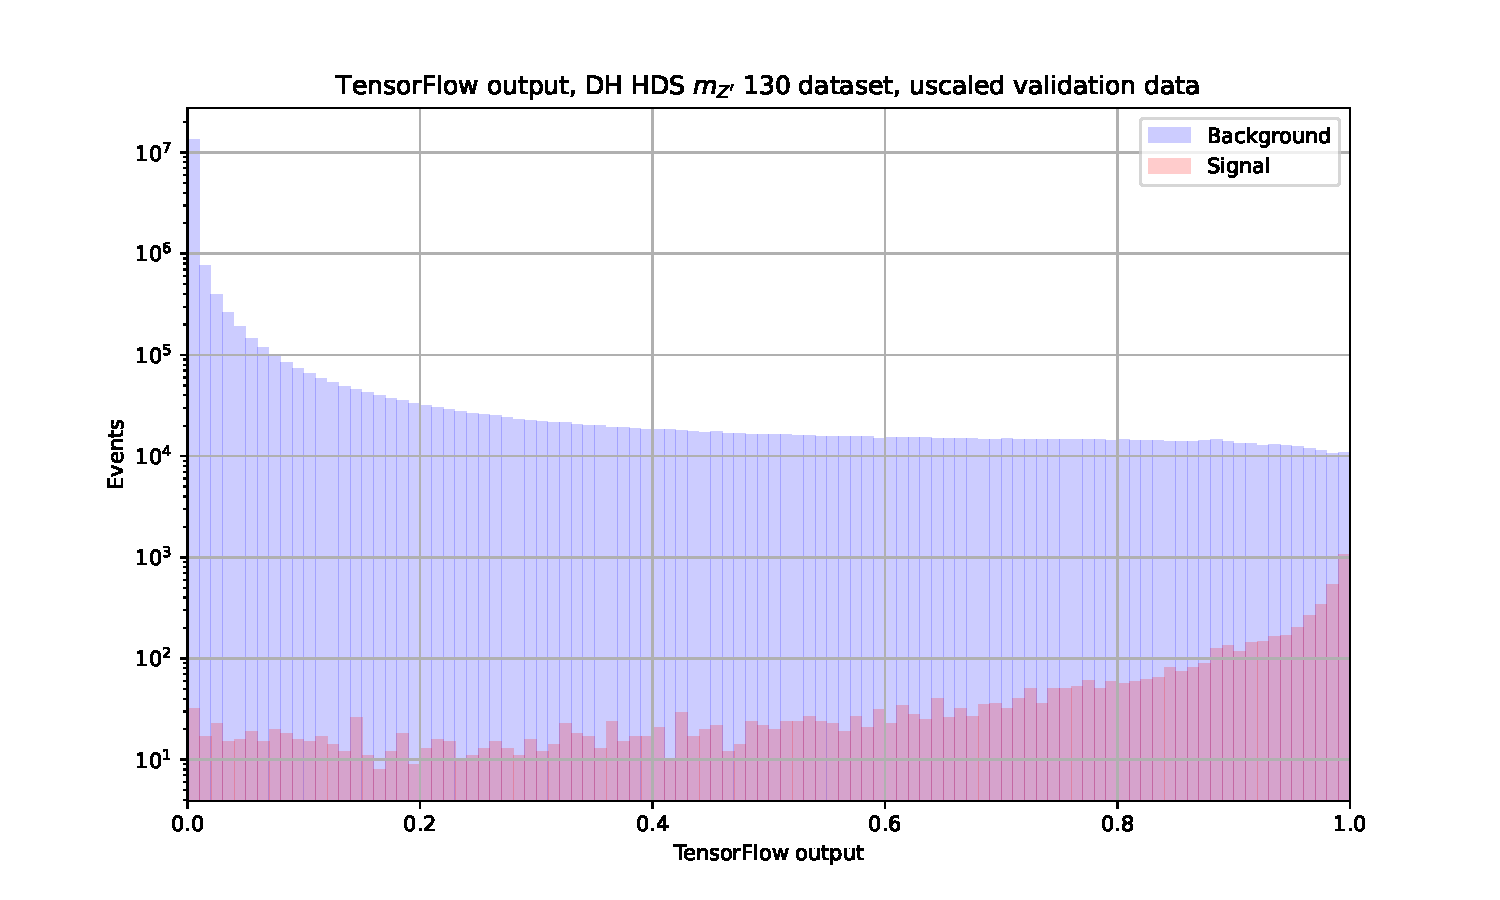
\includegraphics[width=1\textwidth]{DH_HDS_mZp_130/VAL_unscaled.pdf}
        \caption{NN prediction of DH HDS $m_{Z'}$ = 130 GeV}\label{fig:PurelyBalanced_DH_HDS_130}
     \end{subfigure}
     \hfill
     \begin{subfigure}[b]{0.49\textwidth}
        \centering
        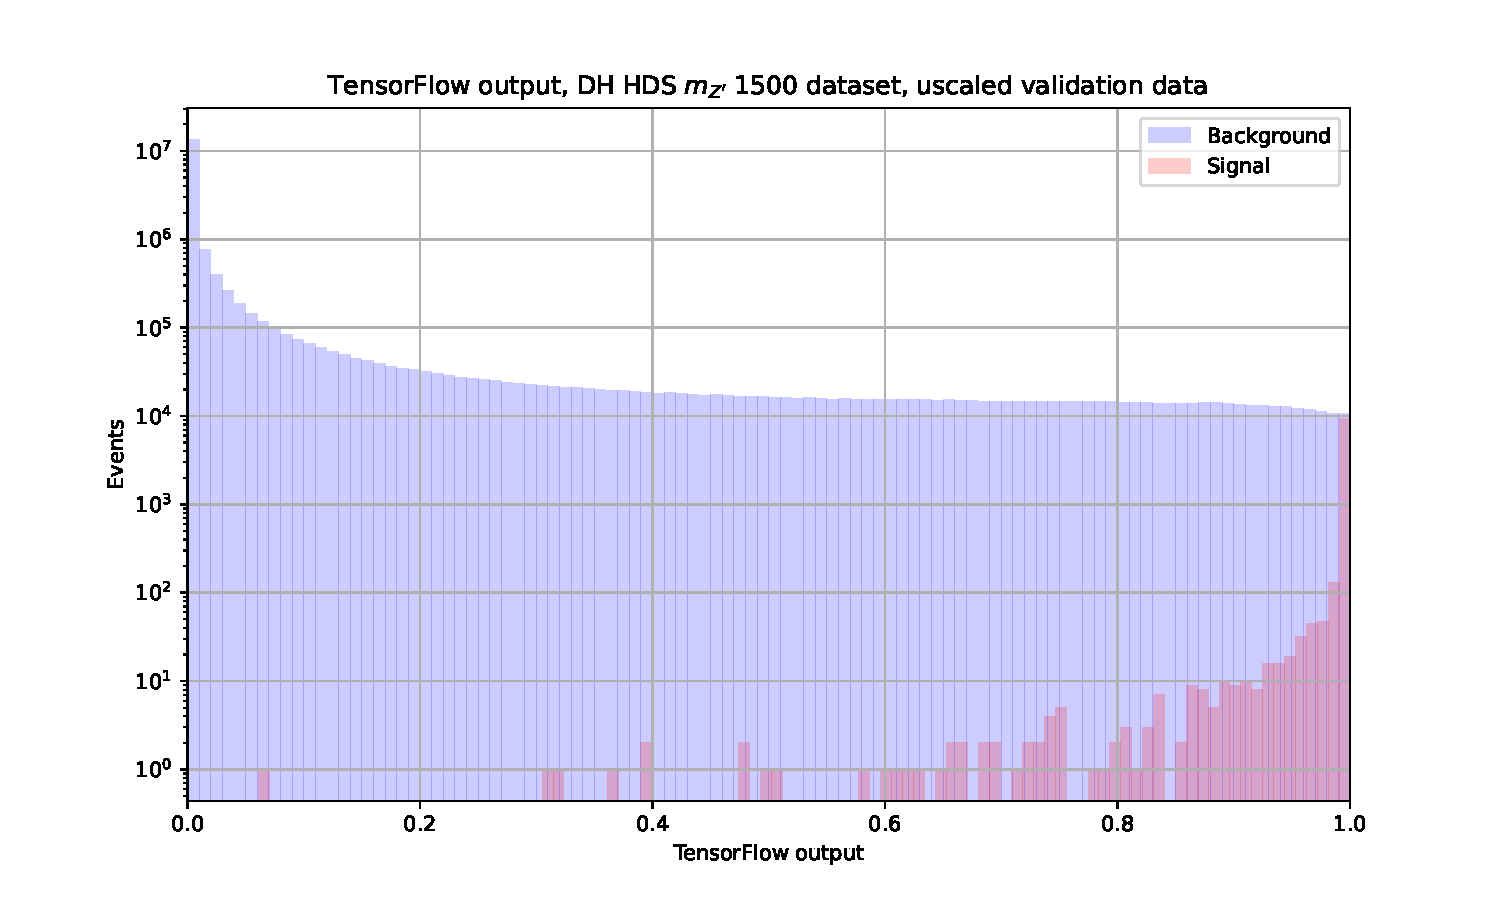
\includegraphics[width=1\textwidth]{DH_HDS_mZp_1500/VAL_unscaled.pdf}
        \caption{NN prediction of DH HDS $m_{Z'}$ = 1500 GeV}\label{fig:PurelyBalanced_DH_HDS_1500}
     \end{subfigure}
     \caption{NN comparison of trained models in FULL Z' dataset}\label{fig:PurelyBalanced_DH_HDS}
\end{figure}
\\The result purely demonstrate the raw network output, meaning that the validation dataset has not been scaled up using MC weights (i.e. model cross section) or luminosity.\\
\\We can see the network is better at classifying the events from the model with $m{Z'}$ = 1500 GeV than the other, even if this model has a much lower cross section, as seen in the correctly scaled plots below.
\begin{figure}[!ht]
	\centering
	\begin{subfigure}[b]{0.49\textwidth}
        \centering
        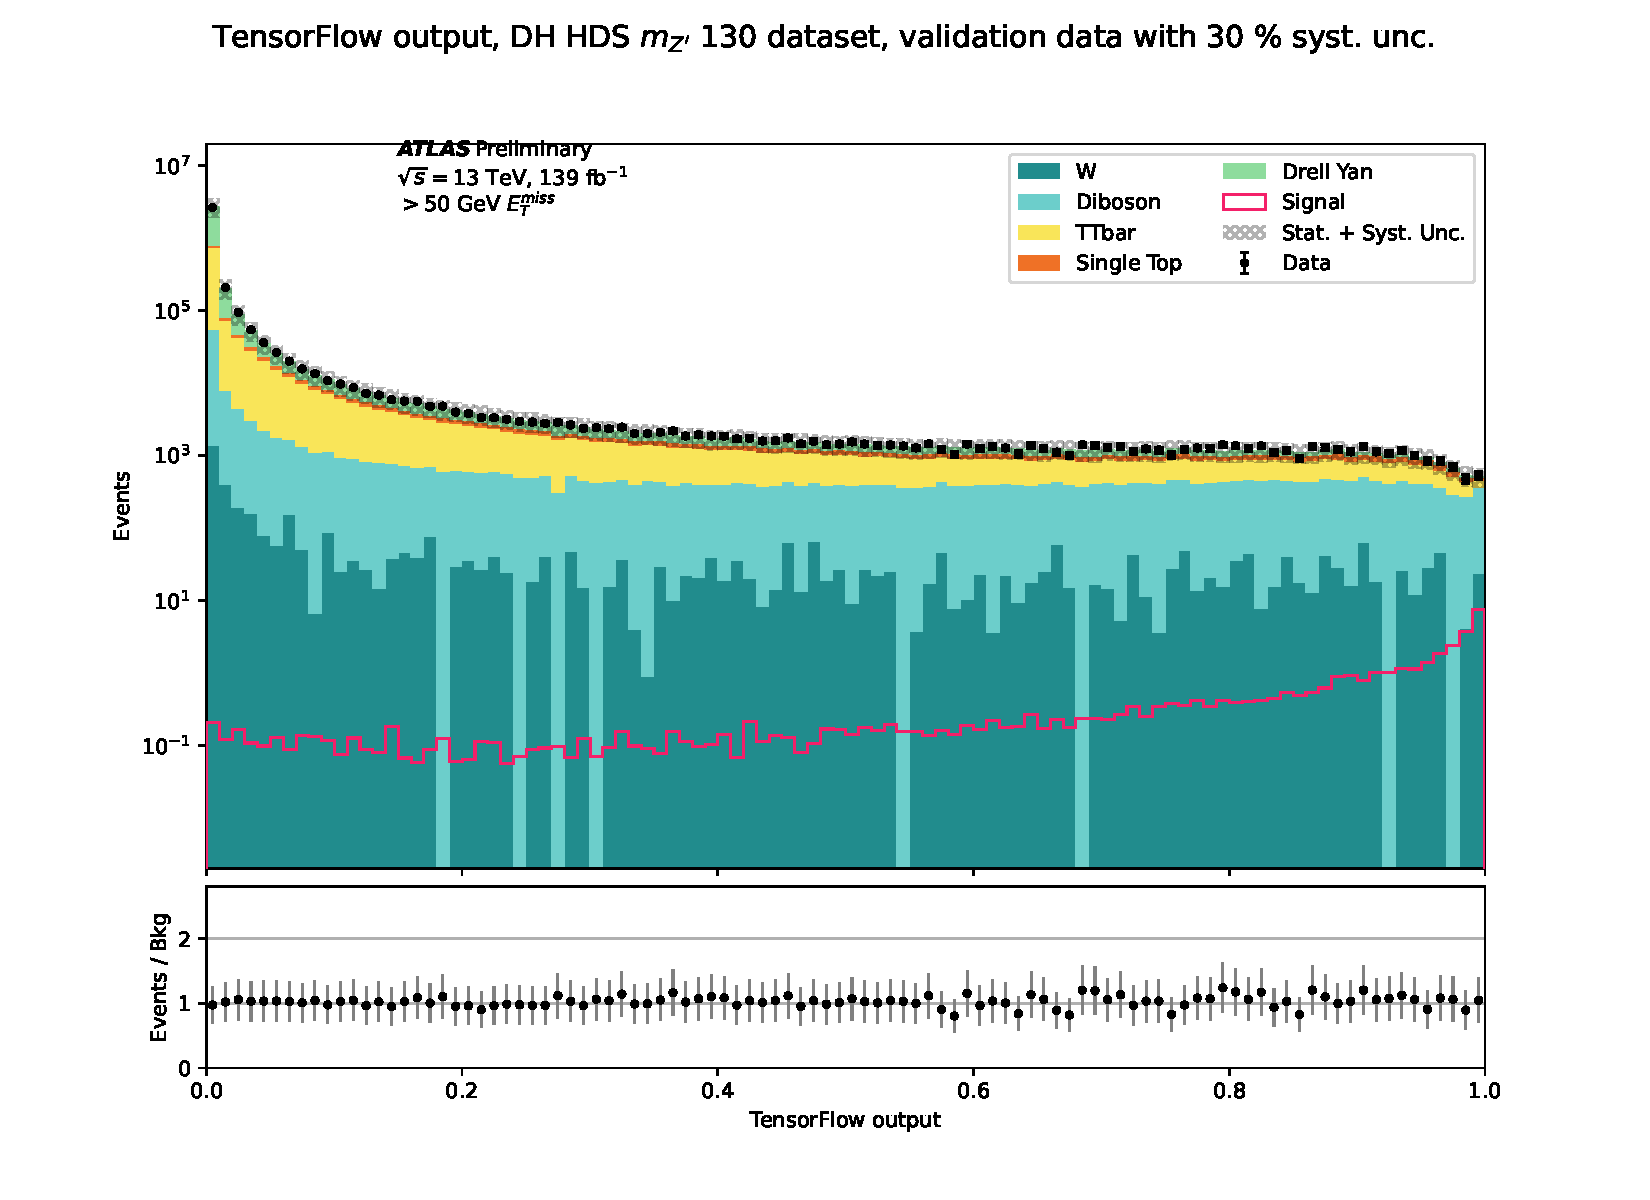
\includegraphics[width=1\textwidth]{DH_HDS_mZp_130/VAL.pdf}
        \caption{NN prediction of DH HDS $m_{Z'}$ = 130 GeV}
     \end{subfigure}
     \hfill
     \begin{subfigure}[b]{0.49\textwidth}
        \centering
        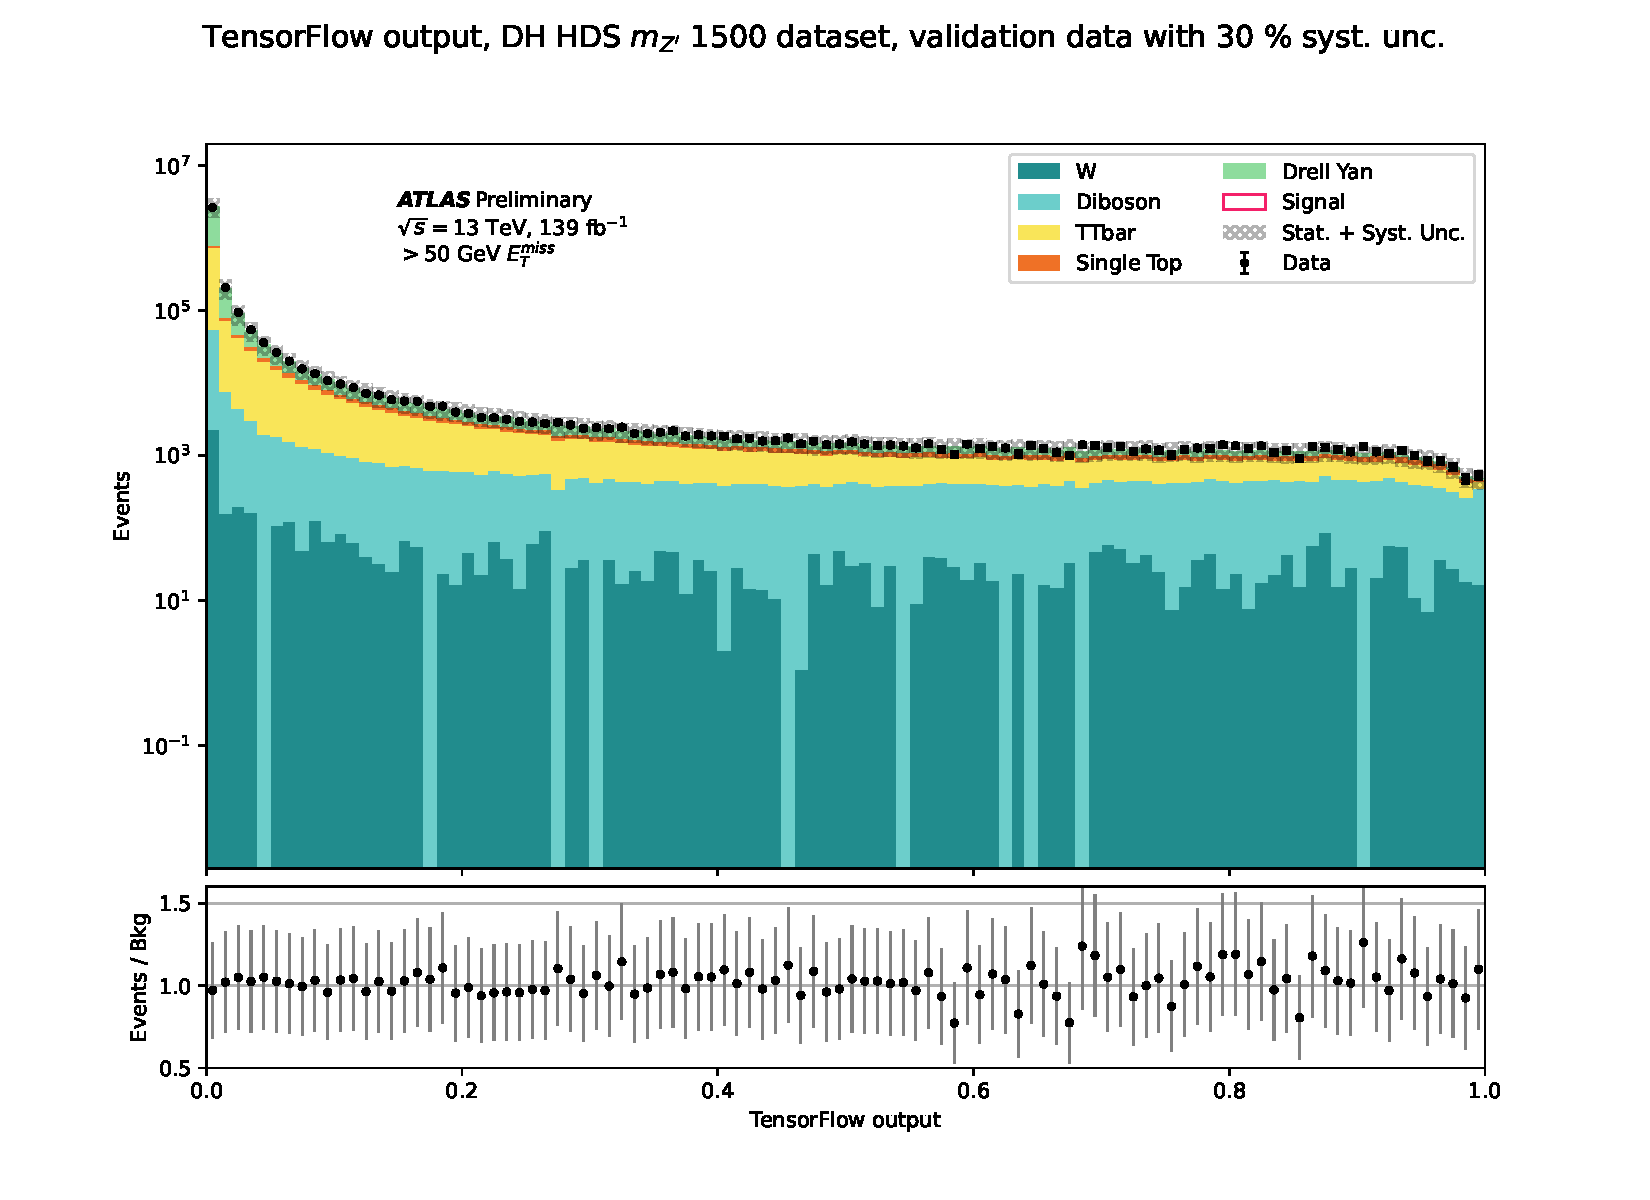
\includegraphics[width=1\textwidth]{DH_HDS_mZp_1500/VAL.pdf}
        \caption{NN prediction of DH HDS $m_{Z'}$ = 1500 GeV}
     \end{subfigure}
     \caption{Correctly scaled plots.}\label{fig:SCALED_PurelyBalanced_DH_HDS}
\end{figure}
\\As we can clearly see, the better predicted model by the network does not even have one event when scaled up correctly. Therefore it is desirable to both take into account the data imbalance between the signal and background as well as the MC weights when training a network. To do this using TensorFlow we could make use of two parameters when training the network: \verb|class_weight| and \verb|sample_weight|.
\\\\\verb|class_weight| works as a dictionary that weights events that are keys on the dictionary. For our purposes we can make a dictionary where we weight signal and background events differently, this is the same type of scaling that was done in the previous section. 
\verb|sample_weight| takes in individual weights for every single event that goes into the netwrok, meaning that it is crucial that we know that the desired weight matches the desired event. Ideally we would use both weighting methods, \verb|class_weight| to balance the signal to background ratio and \verb|sample_weight| with the MC weights. 
However there is a bug in TensorFlow (up to version \verb|GPU 2.7.1|) that makes it so the program doesn't run when using both parameters. This is not a big problem though, as when looking at the source code one can see that what TensorFlow does with both weights is multiply them togheter. Thus we could try to make use of this "balaned weighting" method to see if the network learns the different models better.\\
\\We can see in Table \ref{tab:MC_imbalance} how uneven the data (FULL Z') is. To balance the data we have four options. We can either \textit{weigh up the signal} events by the ratio of background over signal. Or \textit{weigh down the bacgkround} with the ratio of signal over background. However this ratio might differ a lot when using the MC raw event ratio or the SOW events ratio. I have tested all four possibilities and these can be see below.\\
\begin{table}[!h]
   \centering
   \begin{tabular}{l|c|c}\midrule\midrule
                        & Actual events   & MC events \\\midrule
         Background     & 2,715,280.4     & 69,664,290  \\
         Signal         & 388.4           & 2,991,598   \\\midrule\midrule
   \end{tabular}
   \caption[Imbalance raw events and SOW]{Table showcasing the data imbalance between background and signal in both raw MC events and actual events. By actual events it is meant weighted events. This is for the training dataset on the FULL Z' dataset.}
   \label{tab:MC_imbalance}
\end{table}
\graphicspath{{../../../Plots/TESTING/NeuralNetwork/BALANCED_WEIGHTING/MC_WGT_SIG_UP/}}
\begin{figure}[!ht]
	\centering
	\begin{subfigure}[b]{0.49\textwidth}
        \centering
        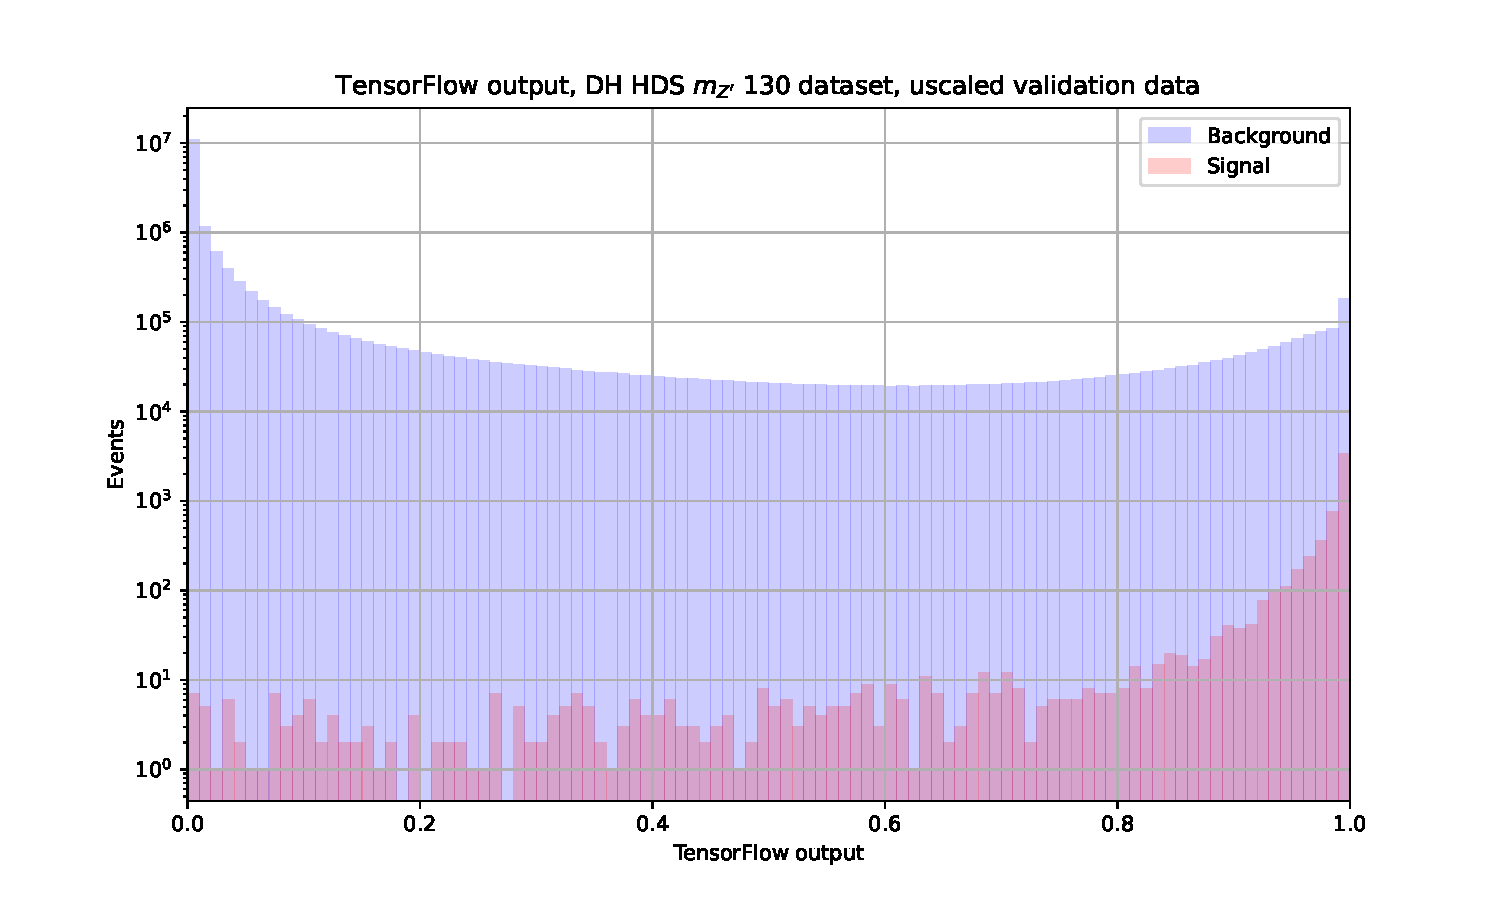
\includegraphics[width=1\textwidth]{DH_HDS_mZp_130/VAL_unscaled.pdf}
        \caption{NN prediction of DH HDS $m_{Z'}$ = 130 GeV}\label{fig:MC_WGT_SIG_DH_HDS_130}
     \end{subfigure}
     \hfill
     \begin{subfigure}[b]{0.49\textwidth}
        \centering
        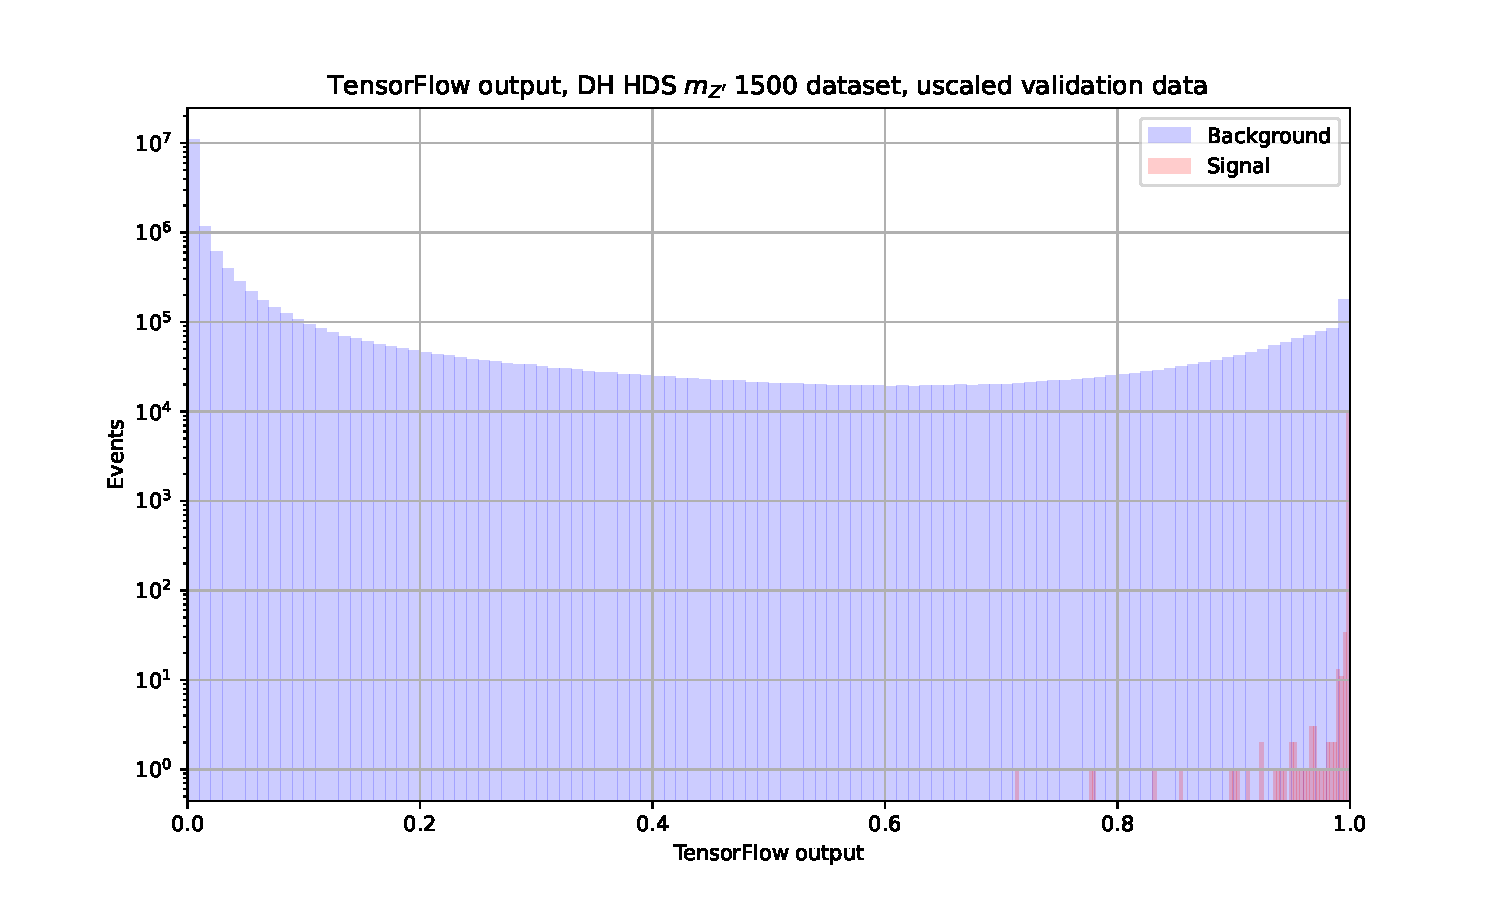
\includegraphics[width=1\textwidth]{DH_HDS_mZp_1500/VAL_unscaled.pdf}
        \caption{NN prediction of DH HDS $m_{Z'}$ = 1500 GeV}\label{fig:MC_WGT_SIG_DH_HDS_1500}
     \end{subfigure}
     \caption{NN prediction when weighting the signal with the SOW ratio.}\label{fig:MC_WGT_SIG_DH_HDS}
\end{figure}
\graphicspath{{../../../Plots/TESTING/NeuralNetwork/BALANCED_WEIGHTING/MC_EVENTS_SIG_UP/}}
\begin{figure}[!ht]
	\centering
	\begin{subfigure}[b]{0.49\textwidth}
        \centering
        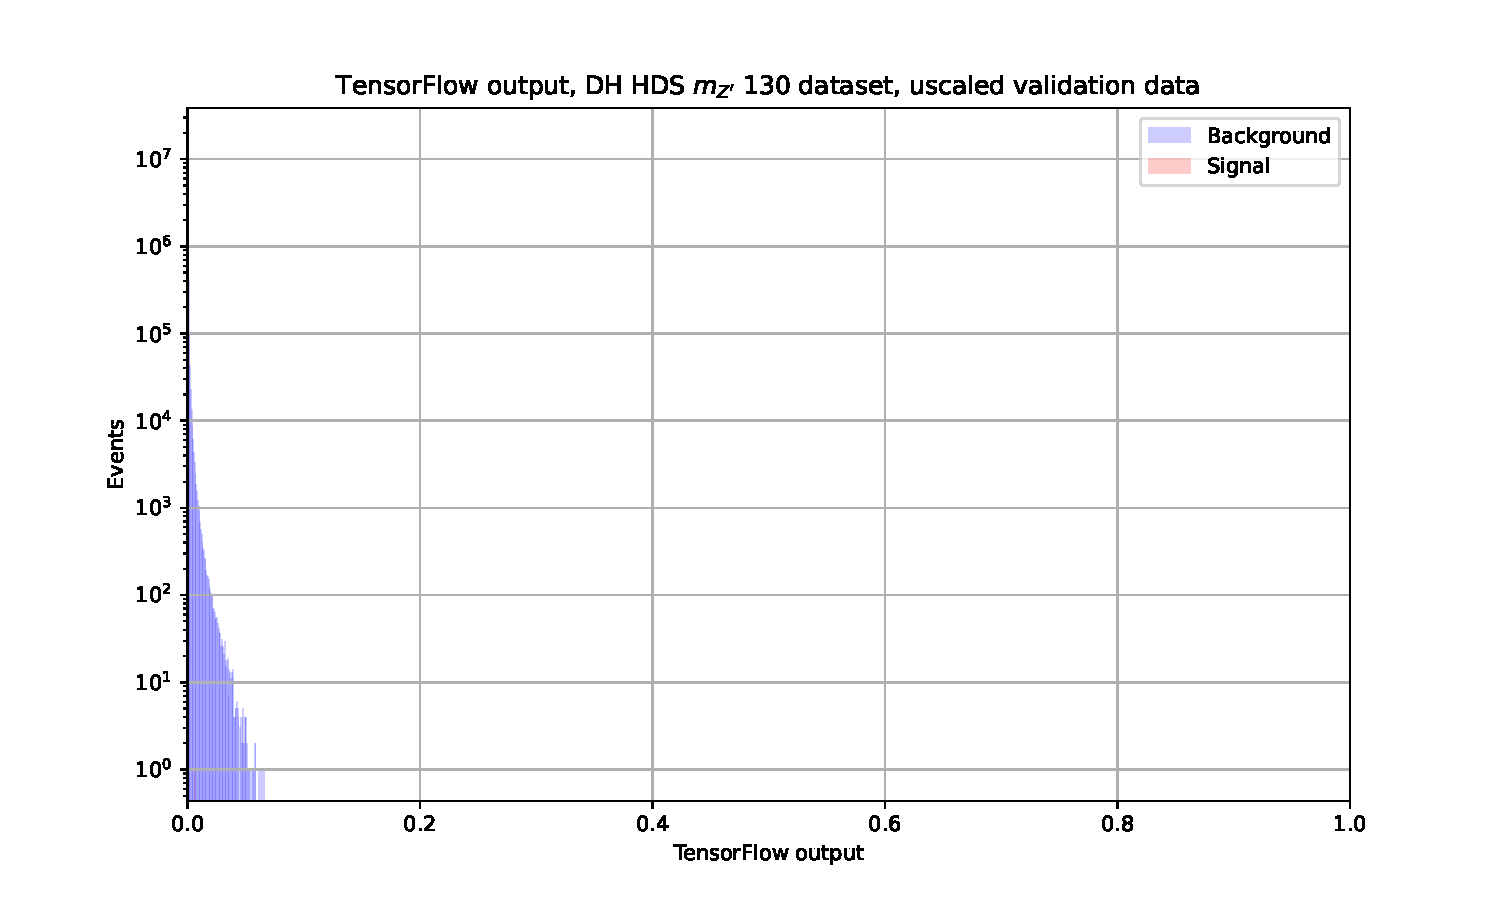
\includegraphics[width=1\textwidth]{DH_HDS_mZp_130/VAL_unscaled.pdf}
        \caption{NN prediction of DH HDS $m_{Z'}$ = 130 GeV}\label{fig:MC_EVT_SIG_DH_HDS_130}
     \end{subfigure}
     \hfill
     \begin{subfigure}[b]{0.49\textwidth}
        \centering
        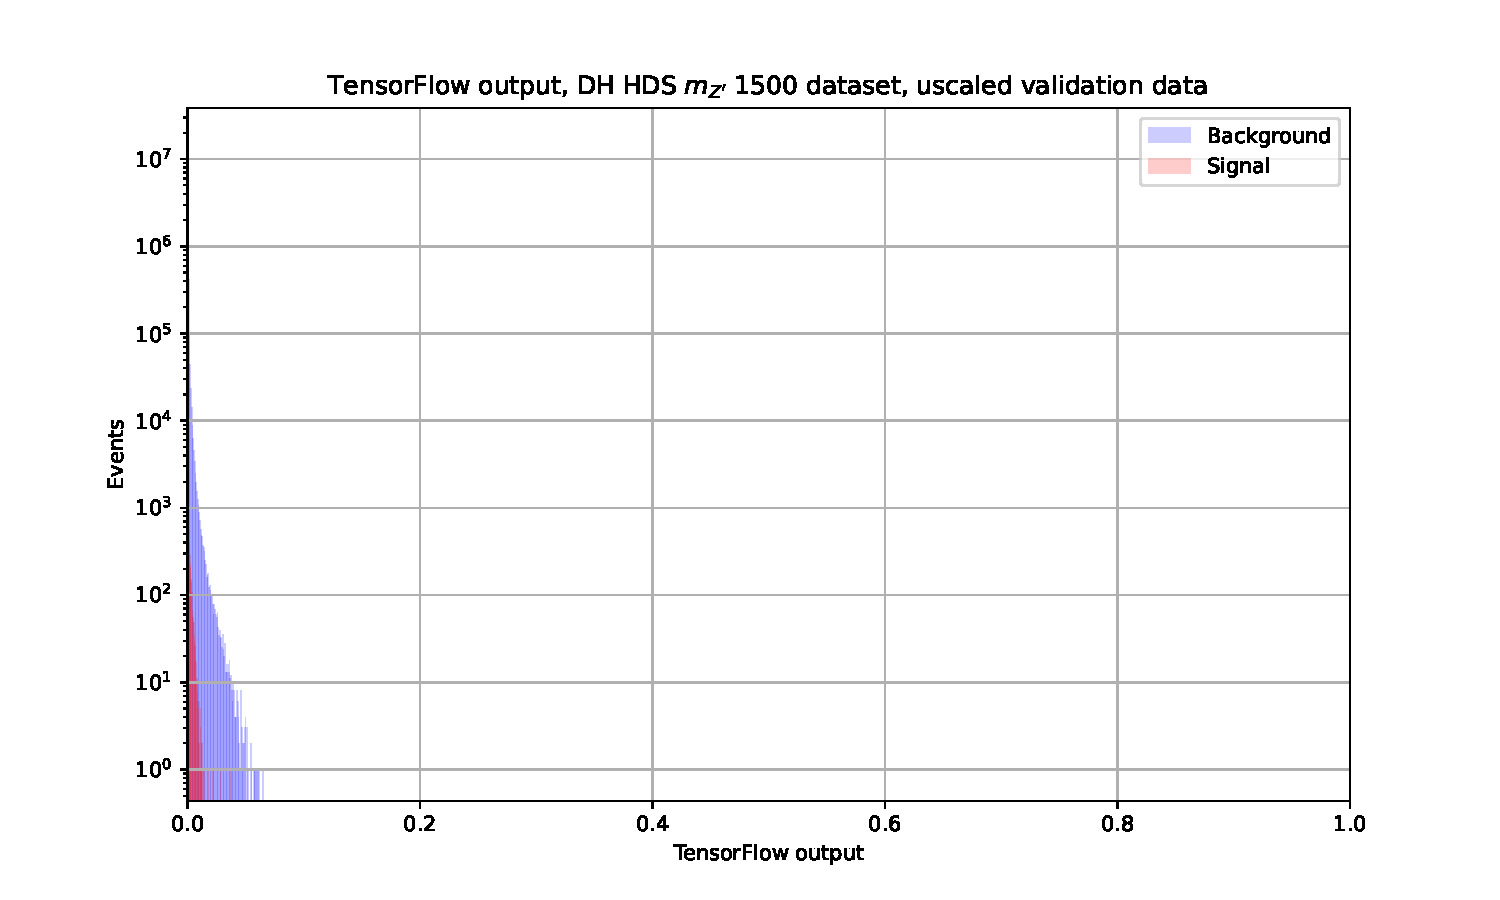
\includegraphics[width=1\textwidth]{DH_HDS_mZp_1500/VAL_unscaled.pdf}
        \caption{NN prediction of DH HDS $m_{Z'}$ = 1500 GeV}\label{fig:MC_EVT_SIG_DH_HDS_1500}
     \end{subfigure}
     \caption{NN prediction when weighting the signal with the raw event ratio.}\label{fig:MC_EVT_SIG_DH_HDS}
\end{figure}
\graphicspath{{../../../Plots/TESTING/NeuralNetwork/BALANCED_WEIGHTING/MC_WGT_BKG_DOWN/}}
\begin{figure}[!ht]
	\centering
	\begin{subfigure}[b]{0.49\textwidth}
        \centering
        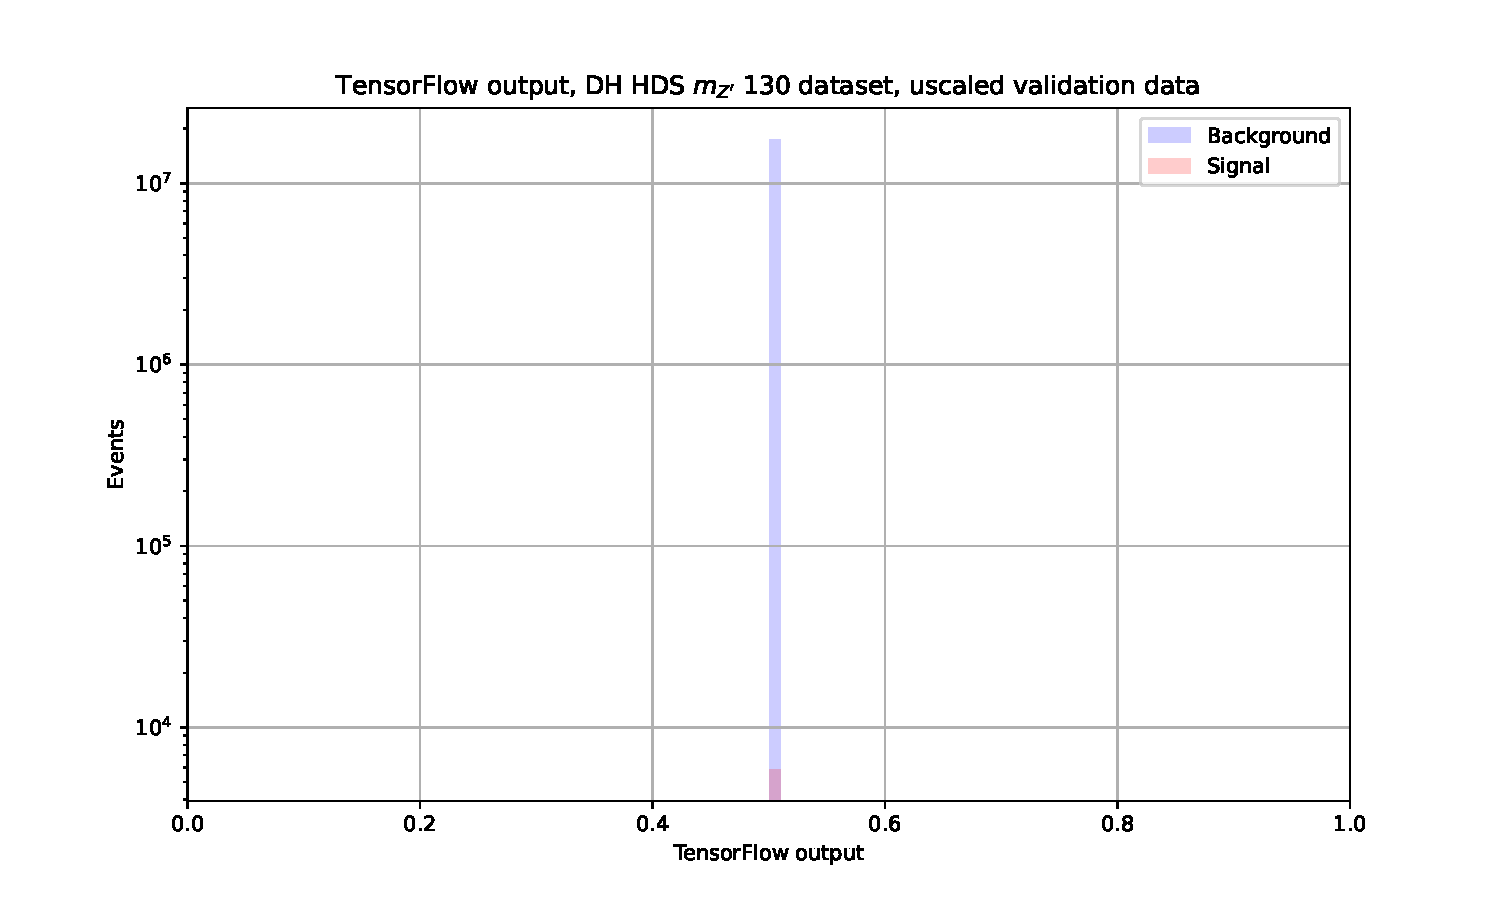
\includegraphics[width=1\textwidth]{DH_HDS_mZp_130/VAL_unscaled.pdf}
        \caption{NN prediction of DH HDS $m_{Z'}$ = 130 GeV}\label{fig:MC_WGT_BKG_DH_HDS_130}
     \end{subfigure}
     \hfill
     \begin{subfigure}[b]{0.49\textwidth}
        \centering
        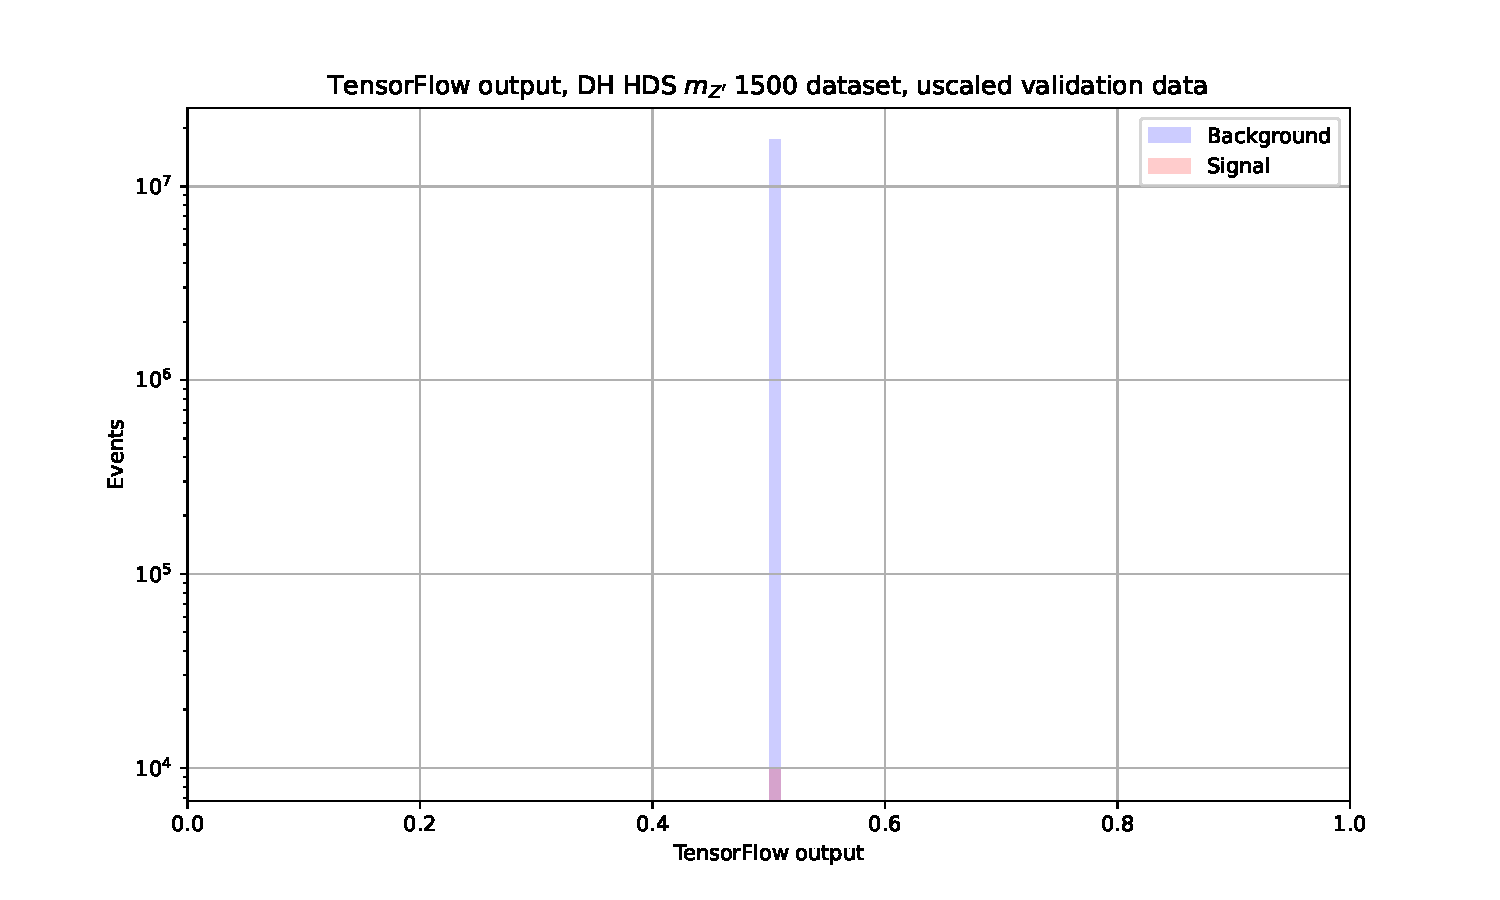
\includegraphics[width=1\textwidth]{DH_HDS_mZp_1500/VAL_unscaled.pdf}
        \caption{NN prediction of DH HDS $m_{Z'}$ = 1500 GeV}\label{fig:MC_WGT_BKG_DH_HDS_1500}
     \end{subfigure}
     \caption{NN prediction when weighting the background with the SOW ratio.}\label{fig:MC_WGT_BKG_DH_HDS}
\end{figure}
\graphicspath{{../../../Plots/TESTING/NeuralNetwork/BALANCED_WEIGHTING/MC_EVENTS_BKG_DOWN/}}
\begin{figure}[!ht]
	\centering
	\begin{subfigure}[b]{0.49\textwidth}
        \centering
        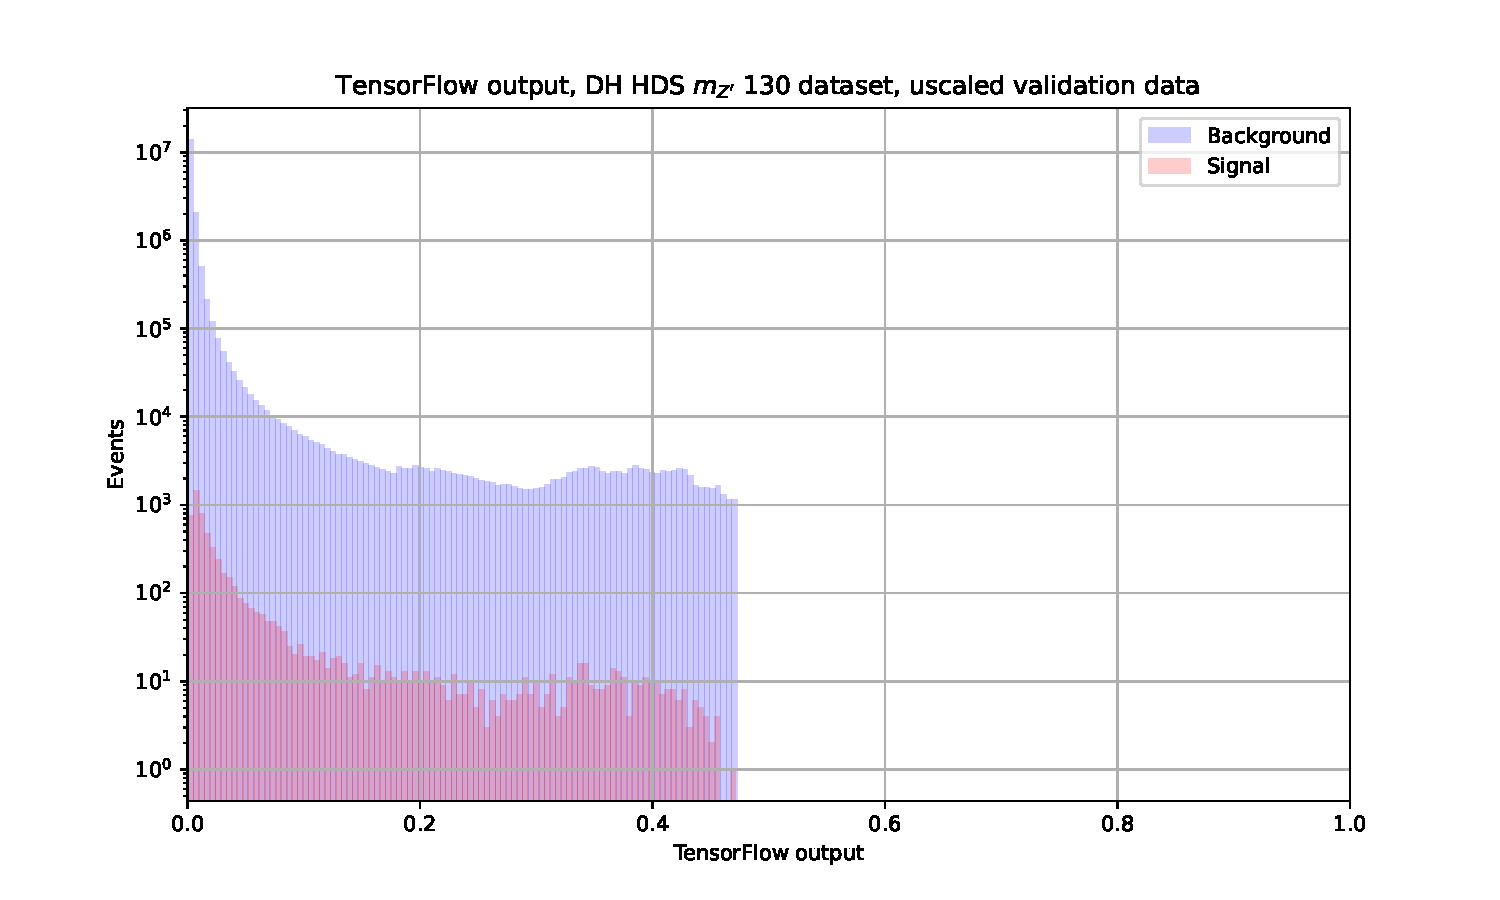
\includegraphics[width=1\textwidth]{DH_HDS_mZp_130/VAL_unscaled.pdf}
        \caption{NN prediction of DH HDS $m_{Z'}$ = 130 GeV}\label{fig:MC_EVT_BKG_DH_HDS_130}
     \end{subfigure}
     \hfill
     \begin{subfigure}[b]{0.49\textwidth}
        \centering
        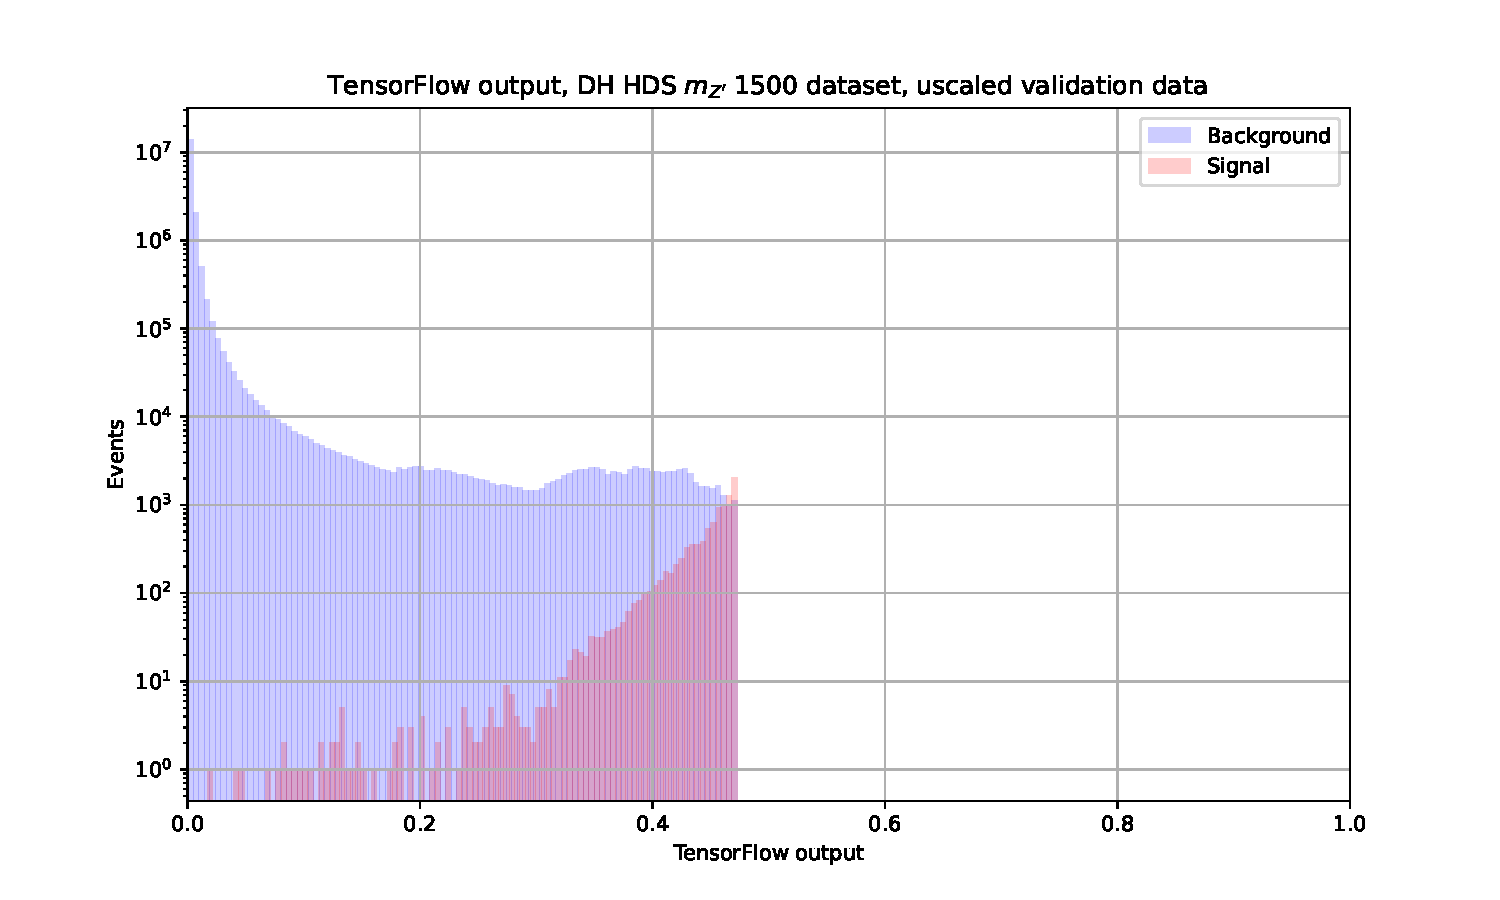
\includegraphics[width=1\textwidth]{DH_HDS_mZp_1500/VAL_unscaled.pdf}
        \caption{NN prediction of DH HDS $m_{Z'}$ = 1500 GeV}\label{fig:MC_EVT_BKG_DH_HDS_1500}
     \end{subfigure}
     \caption{NN prediction when weighting the bacgkround with the raw event ratio.}\label{fig:MC_EVT_BKG_DH_HDS}
\end{figure}
\clearpage 
As we can see almost every way of doing this balanced weighting gives poor results. The only one that seems to work is when we we scale up the MC weights with the ratio between the SOW of the bacgkround over signal, however it does not seem to learn the model with lower mass better compared to how it learned the model with higher mass. It seems to have generally learned both models better, which might be a hint that it learns other models worse, i.e. EFT models with much lower cross section.\\ 
If we now compare the correctly scaled validation plots of DH HDS $m_{Z'}$ = 130 GeV.
\graphicspath{{../../../Plots/TESTING/NeuralNetwork/BALANCED_WEIGHTING/MC_WGT_SIG_UP/}}
\begin{figure}[!ht]
	\centering
	\begin{subfigure}[b]{0.49\textwidth}
        \centering
        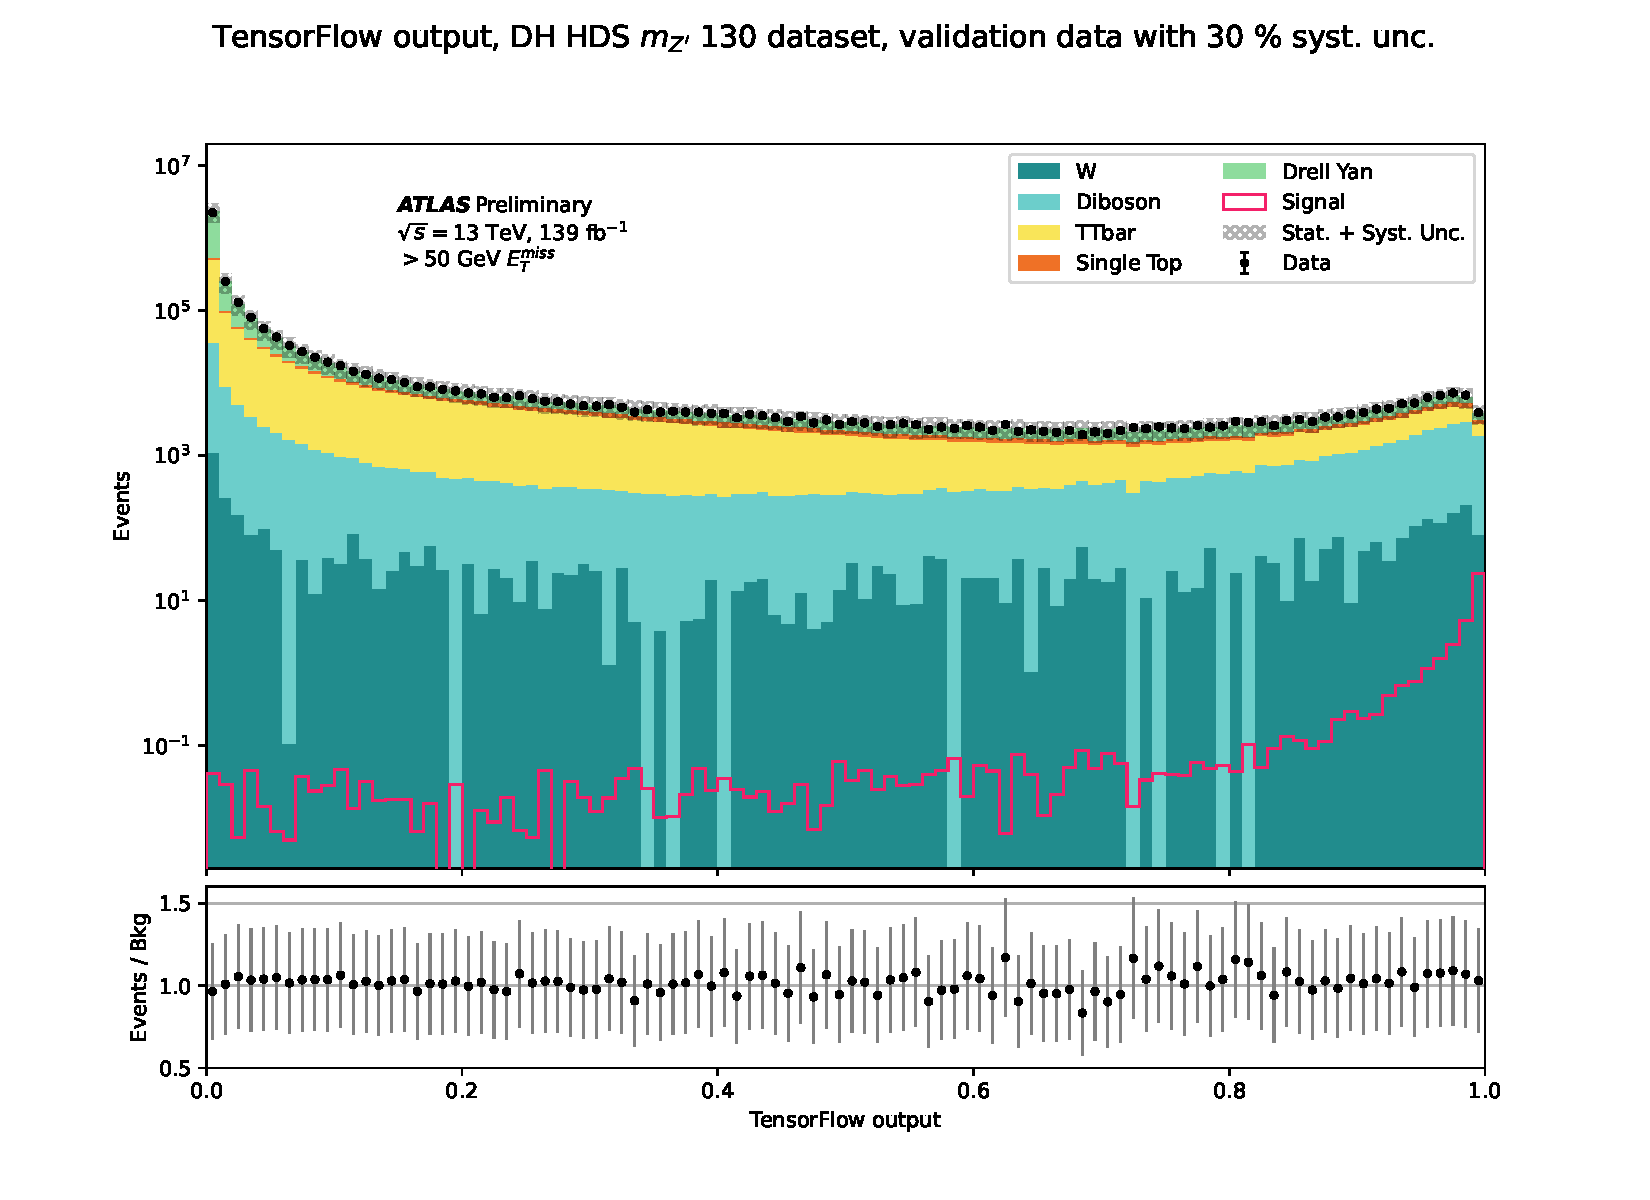
\includegraphics[width=1\textwidth]{DH_HDS_mZp_130/VAL.pdf}
        \caption{MC weights + scaling signal up with SOW ratio}%\label{fig:MC_EVT_BKG_DH_HDS_130}
     \end{subfigure}
     \hfill\graphicspath{{../../../Plots/TESTING/NeuralNetwork/BALANCED_WEIGHTING/ONLY_BALANCE_MC_EVENTS_BKG_DOWN/}}
     \begin{subfigure}[b]{0.49\textwidth}
        \centering
        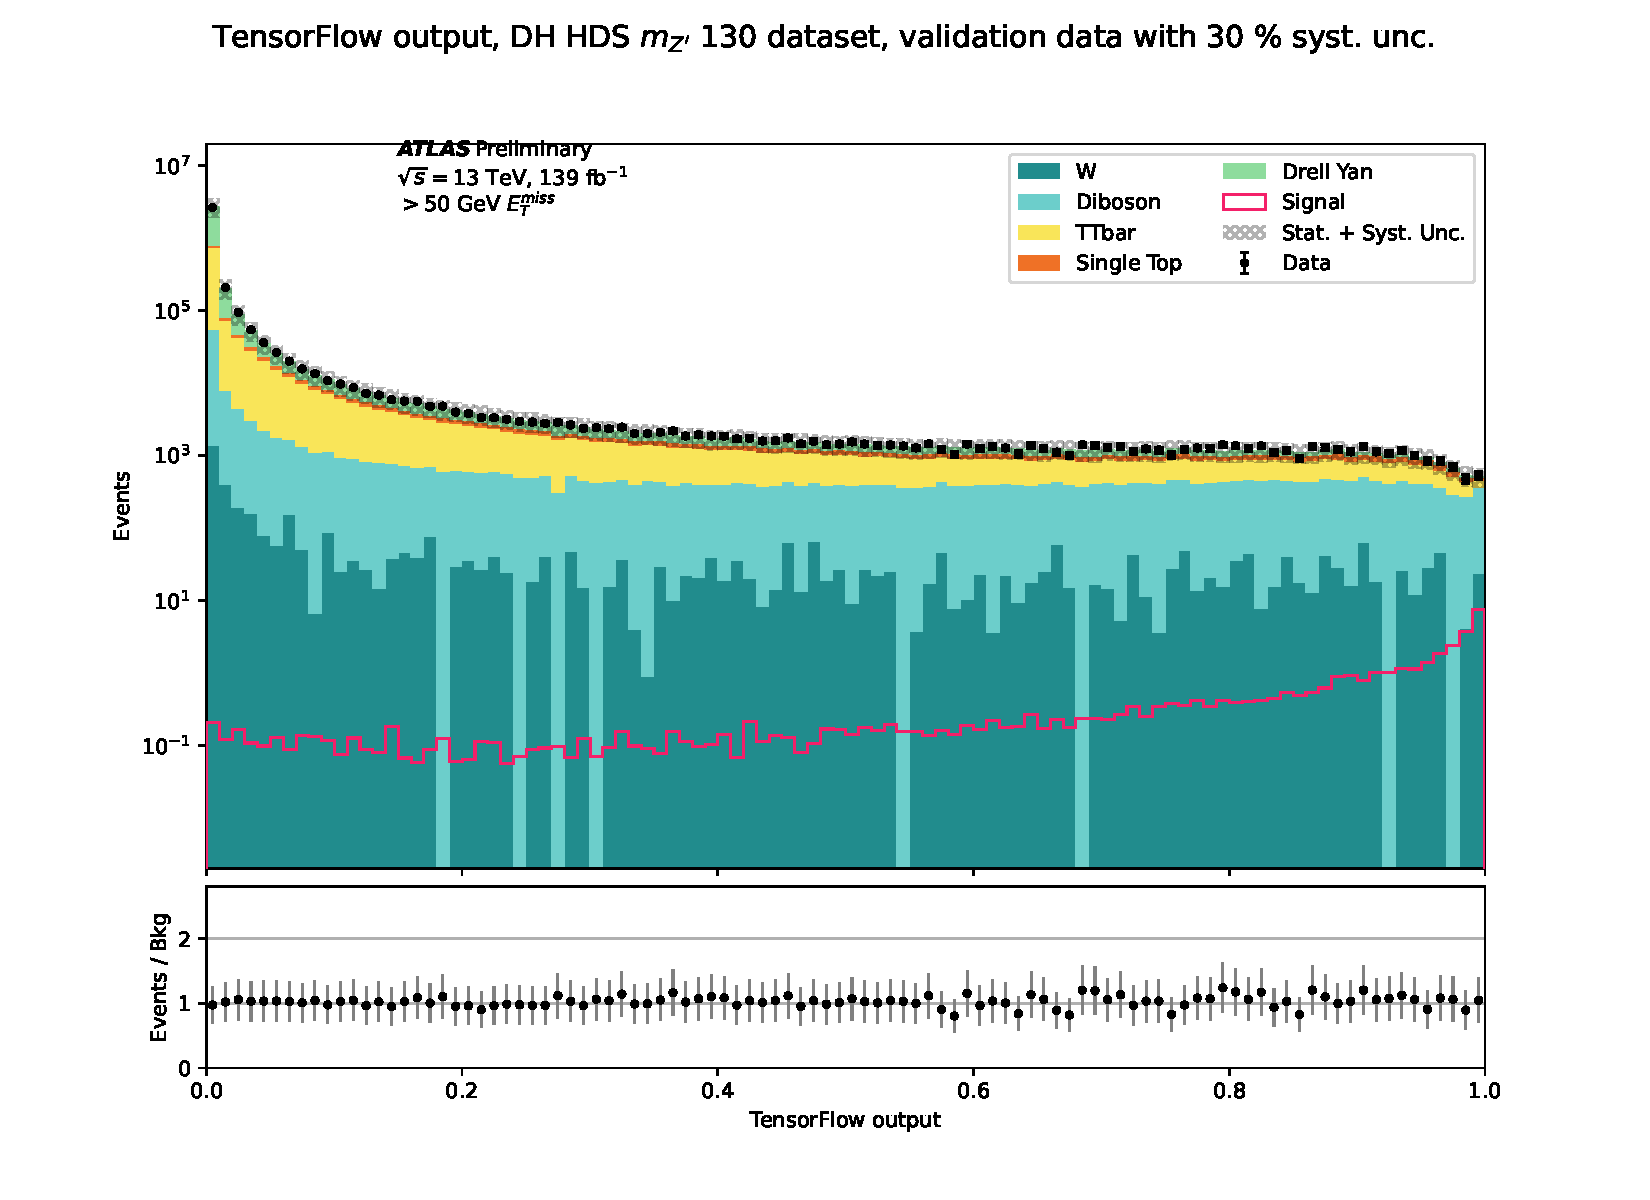
\includegraphics[width=1\textwidth]{DH_HDS_mZp_130/VAL.pdf}
        \caption{Only using raw MC events weigh down bacgkround}%\label{fig:MC_EVT_BKG_DH_HDS_1500}
     \end{subfigure}
   \hfill\graphicspath{{../../../Plots/TESTING/NeuralNetwork/BALANCED_WEIGHTING/MC_WGT_SIG_UP/}}
   \begin{subfigure}[b]{0.49\textwidth}
      \centering
      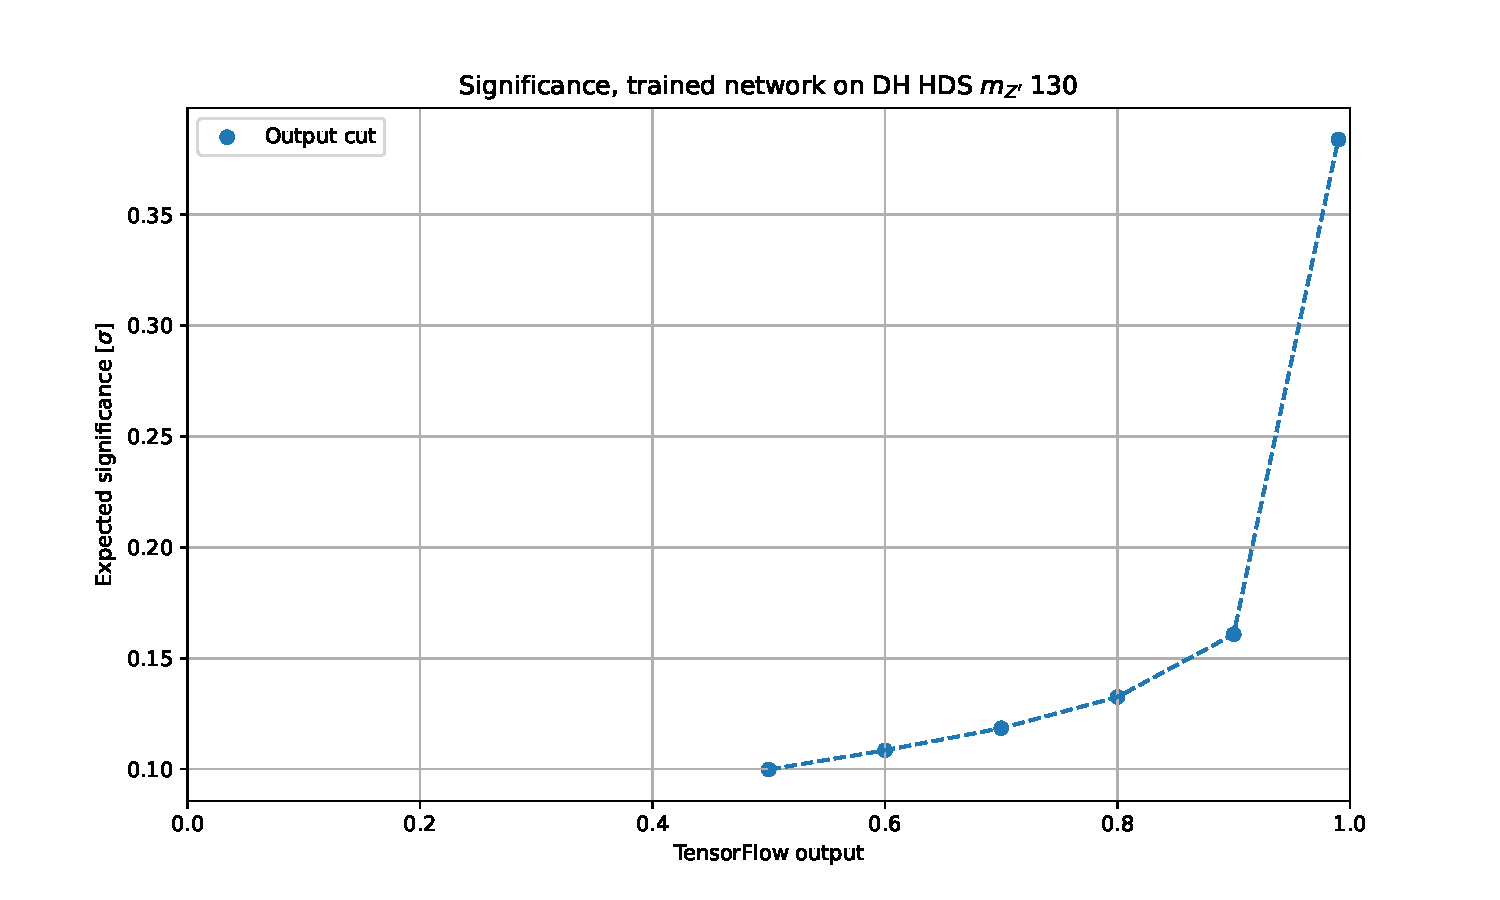
\includegraphics[width=1\textwidth]{DH_HDS_mZp_130/EXP_SIG.pdf}
      \caption{The expected significance of a)}%\label{fig:MC_EVT_BKG_DH_HDS_130}
   \end{subfigure}
   \hfill\graphicspath{{../../../Plots/TESTING/NeuralNetwork/BALANCED_WEIGHTING/ONLY_BALANCE_MC_EVENTS_BKG_DOWN/}}
   \begin{subfigure}[b]{0.49\textwidth}
      \centering
      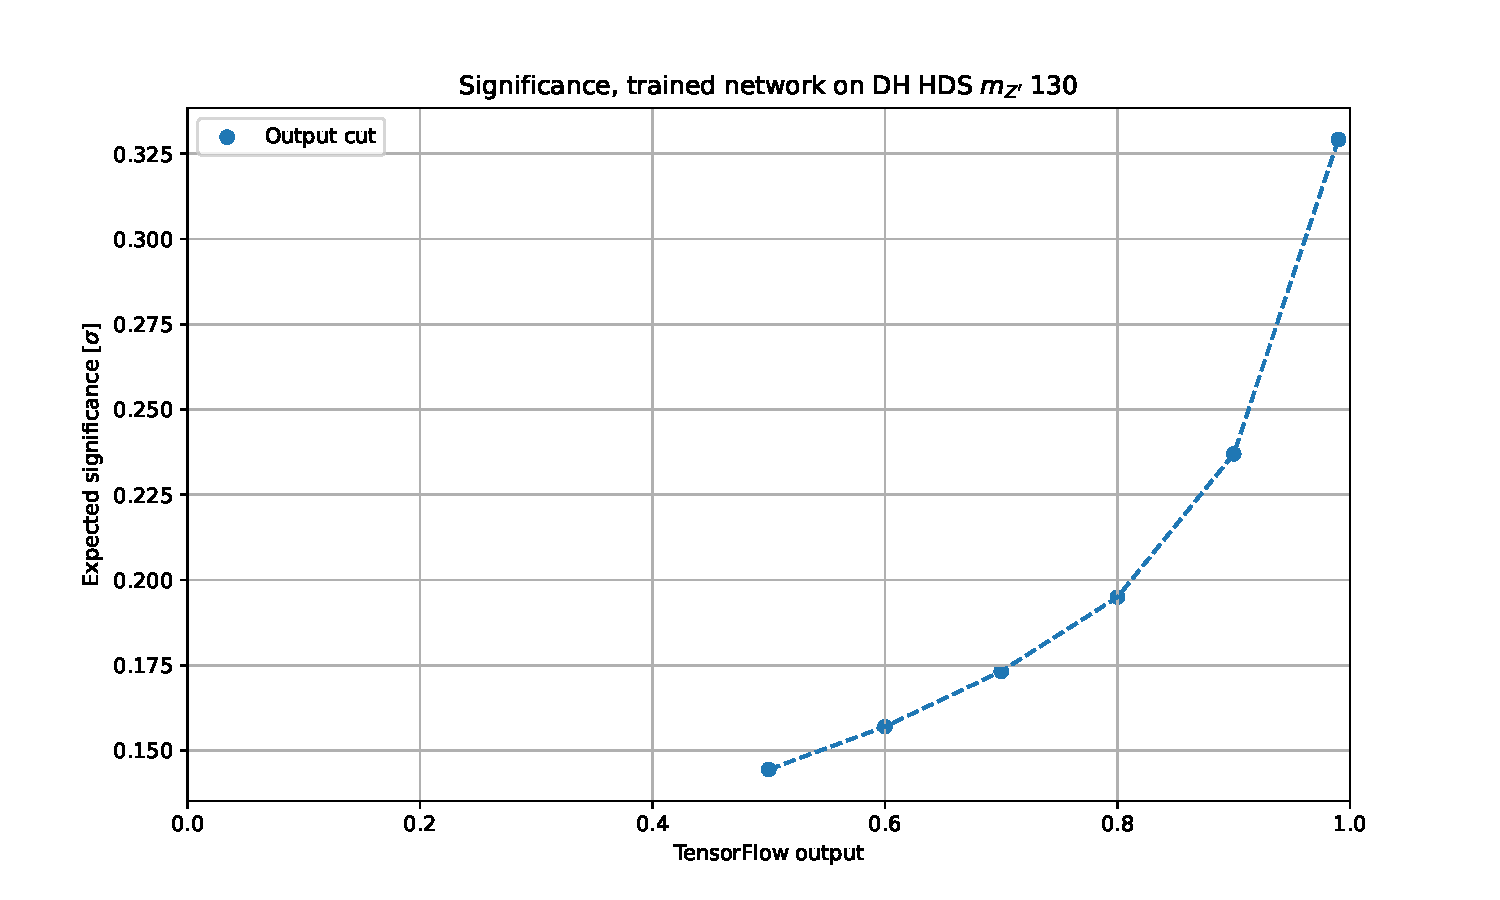
\includegraphics[width=1\textwidth]{DH_HDS_mZp_130/EXP_SIG.pdf}
      \caption{The expected significance of b)}%\label{fig:MC_EVT_BKG_DH_HDS_1500}
   \end{subfigure}
     \caption{Comparison of the best balanced weighting method to the weighting method of the previous section. Figure a) and b) show the validation data of both cases, c) and d) show the expected significance of the validation plots when making a cut on the output. }%\label{fig:MC_EVT_BKG_DH_HDS}
\end{figure}
\\From this we can see that the the network that trained when balancing the data is better at classifying the DH HDS $m_{Z'}$ = 130 GeV model correctly as signal than the other network. We also observe that it wrongly classifies more background as signal than the other network, but even if this is the case the expected significance is greater in the new network.
The reason that the new network wrongly classifies more background as signal might be becuse I utilized the same hyperparameters when training both newtworks, when it might be better to use different hyperparameters on each. 
Another thing that might be of significance is that I used the ratio of the training set, it might make a difference (better or worse) to use the ratio of the full dataset when training as this is more general. 
Since the ratio most likely differs for the training and testing set. \todo{Should I add here that this will not be pursued further? Or rather include it on the "results" part of the thesis}
\clearpage



\subsection{Architecture}\label{sec:NN_Architecture}
The architecture of the NN utilized in this project is of the form shown in Figure \ref{fig:NNArch}.
\begin{figure}[!ht]
   \centering
   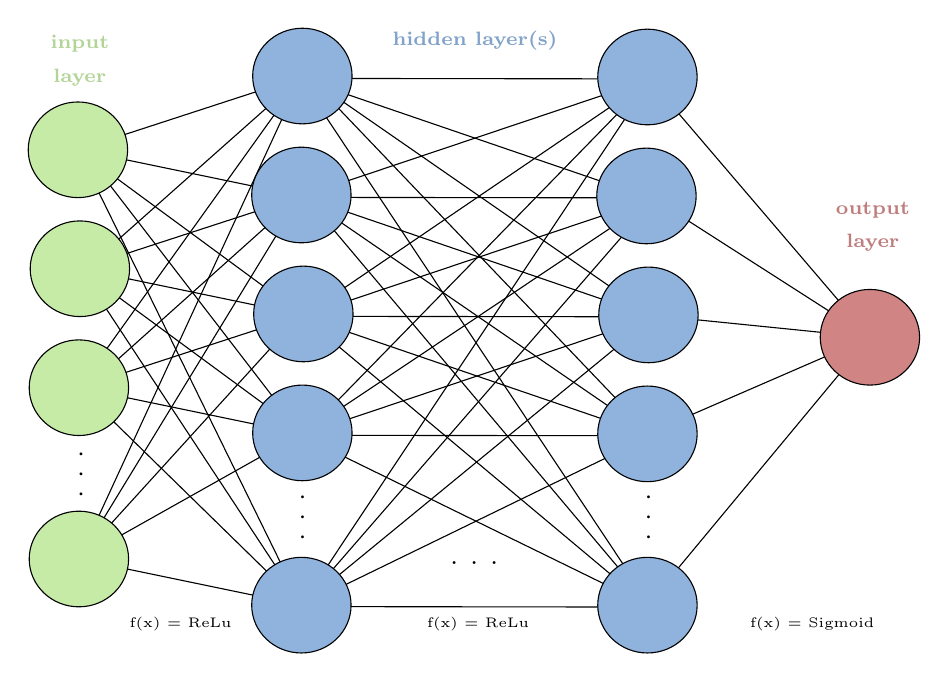
\begin{tikzpicture}[x=0.5pt,y=0.5pt,yscale=-1,xscale=1]
      %uncomment if require: \path (0,496); %set diagram left start at 0, and has height of 496

      %Straight Lines [id:da3125603624631026] 
      \draw    (205.85,243.68) -- (456.31,453.44) ;
      %Straight Lines [id:da4017136284587772] 
      \draw    (44.71,124.36) -- (206.2,71.74) ;
      %Straight Lines [id:da2227878135161746] 
      \draw    (46.14,210.32) -- (207.63,157.71) ;
      %Straight Lines [id:da35416891916640736] 
      \draw    (45.42,296.29) -- (206.92,243.68) ;
      %Straight Lines [id:da16193112504220186] 
      \draw    (45.42,420.09) -- (206.2,329.65) ;
      %Straight Lines [id:da3497039034753928] 
      \draw    (44.71,124.36) -- (205.49,157.71) ;
      %Straight Lines [id:da24573604202629373] 
      \draw    (46.14,210.32) -- (206.92,243.68) ;
      %Straight Lines [id:da01718938654762414] 
      \draw    (45.42,296.29) -- (206.2,329.65) ;
      %Straight Lines [id:da4694218304226967] 
      \draw    (45.42,420.09) -- (206.2,453.44) ;
      %Straight Lines [id:da6780505366621903] 
      \draw    (44.71,124.36) -- (206.92,243.68) ;
      %Straight Lines [id:da3700806633588325] 
      \draw    (46.14,210.32) -- (208.35,329.65) ;
      %Straight Lines [id:da7204661169538961] 
      \draw    (45.42,296.29) -- (206.2,453.44) ;
      %Straight Lines [id:da03352111792760715] 
      \draw    (49.89,126.59) -- (206.2,329.65) ;
      %Straight Lines [id:da7880697711535636] 
      \draw    (44.71,124.36) -- (206.2,453.44) ;
      %Straight Lines [id:da8177807044758987] 
      \draw    (46.14,210.32) -- (206.2,453.44) ;
      %Straight Lines [id:da5902292990985858] 
      \draw    (49.89,210.5) -- (206.2,71.74) ;
      %Straight Lines [id:da7293359024356544] 
      \draw    (45.42,296.29) -- (206.2,71.74) ;
      %Straight Lines [id:da8672682409124693] 
      \draw    (45.42,420.09) -- (206.2,71.74) ;
      %Straight Lines [id:da14015258542164877] 
      \draw    (52.03,295.09) -- (205.49,157.71) ;
      %Straight Lines [id:da6510778766409582] 
      \draw    (45.42,420.09) -- (205.49,157.71) ;
      %Straight Lines [id:da19048953930291812] 
      \draw    (45.42,420.09) -- (205.85,243.68) ;
      %Straight Lines [id:da5900414918521127] 
      \draw    (205.52,72.77) -- (459.29,73.12) ;
      %Straight Lines [id:da9923475282888197] 
      \draw    (204.06,158.74) -- (459.29,73.12) ;
      %Straight Lines [id:da6224502087859033] 
      \draw    (206.98,244.71) -- (462.21,159.09) ;
      %Straight Lines [id:da21387151774072322] 
      \draw    (205.52,330.68) -- (460.75,245.05) ;
      %Straight Lines [id:da40912543404428503] 
      \draw    (205.52,454.47) -- (459.29,331.02) ;
      %Straight Lines [id:da6756606943081097] 
      \draw    (208.44,158.74) -- (462.21,159.09) ;
      %Straight Lines [id:da16137493446626694] 
      \draw    (206.98,244.71) -- (460.75,245.05) ;
      %Straight Lines [id:da10150687813127202] 
      \draw    (205.52,330.68) -- (459.29,331.02) ;
      %Straight Lines [id:da0030866090013578207] 
      \draw    (205.52,454.47) -- (459.29,454.82) ;
      %Straight Lines [id:da5047969586038915] 
      \draw    (206.98,244.71) -- (459.29,73.12) ;
      %Straight Lines [id:da16781805884673007] 
      \draw    (204.43,334.29) -- (459.29,73.12) ;
      %Straight Lines [id:da5565130910620758] 
      \draw    (205.52,454.47) -- (459.29,73.12) ;
      %Straight Lines [id:da36371826499194726] 
      \draw    (205.52,454.47) -- (462.21,159.09) ;
      %Straight Lines [id:da11821496918512042] 
      \draw    (205.52,330.68) -- (462.21,159.09) ;
      %Straight Lines [id:da7692636391915034] 
      \draw    (205.52,72.77) -- (457.83,159.09) ;
      %Straight Lines [id:da6770318174394677] 
      \draw    (208.44,158.74) -- (460.75,245.05) ;
      %Straight Lines [id:da9309923147992141] 
      \draw    (206.98,244.71) -- (459.29,331.02) ;
      %Straight Lines [id:da7413198534186101] 
      \draw    (213.18,73.63) -- (460.75,245.05) ;
      %Straight Lines [id:da26068921273410117] 
      \draw    (213.18,73.63) -- (459.29,331.02) ;
      %Straight Lines [id:da8585525579192329] 
      \draw    (205.52,72.77) -- (459.29,454.82) ;
      %Straight Lines [id:da2270863173532055] 
      \draw    (213.18,162.87) -- (459.29,454.82) ;
      %Straight Lines [id:da5864780819119888] 
      \draw    (205.52,330.68) -- (459.29,454.82) ;
      %Straight Lines [id:da16348930210331503] 
      \draw    (205.52,454.47) -- (460.75,245.05) ;
      %Straight Lines [id:da2425074417898001] 
      \draw    (208.44,158.74) -- (459.29,331.02) ;
      %Straight Lines [id:da13422732156968453] 
      \draw    (456.31,71.74) -- (617.09,259.84) ;
      %Straight Lines [id:da7308781194762678] 
      \draw    (457.74,157.71) -- (617.09,259.84) ;
      %Straight Lines [id:da5359704776892366] 
      \draw    (457.02,243.68) -- (617.09,259.84) ;
      %Straight Lines [id:da3406152128273612] 
      \draw    (456.31,329.65) -- (617.09,259.84) ;
      %Straight Lines [id:da14904168253418448] 
      \draw    (456.31,453.44) -- (617.09,259.84) ;
      %Shape: Ellipse [id:dp8560274429988182] 
      \draw  [fill={rgb, 255:red, 198; green, 235; blue, 167 }  ,fill opacity=1 ] (8.8,124.36) .. controls (8.8,105.27) and (24.88,89.8) .. (44.71,89.8) .. controls (64.54,89.8) and (80.62,105.27) .. (80.62,124.36) .. controls (80.62,143.44) and (64.54,158.91) .. (44.71,158.91) .. controls (24.88,158.91) and (8.8,143.44) .. (8.8,124.36) -- cycle ;
      %Shape: Ellipse [id:dp5971121909630736] 
      \draw  [fill={rgb, 255:red, 198; green, 235; blue, 167 }  ,fill opacity=1 ] (10.23,210.32) .. controls (10.23,191.24) and (26.31,175.76) .. (46.14,175.76) .. controls (65.97,175.76) and (82.05,191.24) .. (82.05,210.32) .. controls (82.05,229.41) and (65.97,244.88) .. (46.14,244.88) .. controls (26.31,244.88) and (10.23,229.41) .. (10.23,210.32) -- cycle ;
      %Shape: Ellipse [id:dp024903598729203225] 
      \draw  [fill={rgb, 255:red, 198; green, 235; blue, 167 }  ,fill opacity=1 ] (9.51,296.29) .. controls (9.51,277.21) and (25.59,261.73) .. (45.42,261.73) .. controls (65.25,261.73) and (81.33,277.21) .. (81.33,296.29) .. controls (81.33,315.38) and (65.25,330.85) .. (45.42,330.85) .. controls (25.59,330.85) and (9.51,315.38) .. (9.51,296.29) -- cycle ;
      %Shape: Ellipse [id:dp2752980849146809] 
      \draw  [fill={rgb, 255:red, 198; green, 235; blue, 167 }  ,fill opacity=1 ] (9.51,420.09) .. controls (9.51,401) and (25.59,385.53) .. (45.42,385.53) .. controls (65.25,385.53) and (81.33,401) .. (81.33,420.09) .. controls (81.33,439.17) and (65.25,454.64) .. (45.42,454.64) .. controls (25.59,454.64) and (9.51,439.17) .. (9.51,420.09) -- cycle ;

      %Shape: Ellipse [id:dp22212680764969794] 
      \draw  [fill={rgb, 255:red, 143; green, 179; blue, 221 }  ,fill opacity=1 ] (171.01,71.06) .. controls (171.01,51.97) and (187.09,36.5) .. (206.92,36.5) .. controls (226.75,36.5) and (242.83,51.97) .. (242.83,71.06) .. controls (242.83,90.14) and (226.75,105.61) .. (206.92,105.61) .. controls (187.09,105.61) and (171.01,90.14) .. (171.01,71.06) -- cycle ;
      %Shape: Ellipse [id:dp31615925311964466] 
      \draw  [fill={rgb, 255:red, 143; green, 179; blue, 221 }  ,fill opacity=1 ] (170.3,157.02) .. controls (170.3,137.94) and (186.37,122.46) .. (206.2,122.46) .. controls (226.04,122.46) and (242.11,137.94) .. (242.11,157.02) .. controls (242.11,176.11) and (226.04,191.58) .. (206.2,191.58) .. controls (186.37,191.58) and (170.3,176.11) .. (170.3,157.02) -- cycle ;
      %Shape: Ellipse [id:dp763257580789] 
      \draw  [fill={rgb, 255:red, 143; green, 179; blue, 221 }  ,fill opacity=1 ] (171.73,242.99) .. controls (171.73,223.9) and (187.8,208.43) .. (207.63,208.43) .. controls (227.47,208.43) and (243.54,223.9) .. (243.54,242.99) .. controls (243.54,262.08) and (227.47,277.55) .. (207.63,277.55) .. controls (187.8,277.55) and (171.73,262.08) .. (171.73,242.99) -- cycle ;
      %Shape: Ellipse [id:dp41332126656266754] 
      \draw  [fill={rgb, 255:red, 143; green, 179; blue, 221 }  ,fill opacity=1 ] (171.01,328.96) .. controls (171.01,309.87) and (187.09,294.4) .. (206.92,294.4) .. controls (226.75,294.4) and (242.83,309.87) .. (242.83,328.96) .. controls (242.83,348.05) and (226.75,363.52) .. (206.92,363.52) .. controls (187.09,363.52) and (171.01,348.05) .. (171.01,328.96) -- cycle ;
      %Shape: Ellipse [id:dp3269904901419234] 
      \draw  [fill={rgb, 255:red, 143; green, 179; blue, 221 }  ,fill opacity=1 ] (170.3,453.44) .. controls (170.3,434.35) and (186.37,418.88) .. (206.2,418.88) .. controls (226.04,418.88) and (242.11,434.35) .. (242.11,453.44) .. controls (242.11,472.53) and (226.04,488) .. (206.2,488) .. controls (186.37,488) and (170.3,472.53) .. (170.3,453.44) -- cycle ;
      %Shape: Ellipse [id:dp43598218516443177] 
      \draw  [fill={rgb, 255:red, 143; green, 179; blue, 221 }  ,fill opacity=1 ] (420.4,71.74) .. controls (420.4,52.66) and (436.48,37.18) .. (456.31,37.18) .. controls (476.14,37.18) and (492.22,52.66) .. (492.22,71.74) .. controls (492.22,90.83) and (476.14,106.3) .. (456.31,106.3) .. controls (436.48,106.3) and (420.4,90.83) .. (420.4,71.74) -- cycle ;
      %Shape: Ellipse [id:dp5839593265260355] 
      \draw  [fill={rgb, 255:red, 143; green, 179; blue, 221 }  ,fill opacity=1 ] (419.69,157.71) .. controls (419.69,138.62) and (435.76,123.15) .. (455.6,123.15) .. controls (475.43,123.15) and (491.5,138.62) .. (491.5,157.71) .. controls (491.5,176.8) and (475.43,192.27) .. (455.6,192.27) .. controls (435.76,192.27) and (419.69,176.8) .. (419.69,157.71) -- cycle ;
      %Shape: Ellipse [id:dp5046190422661424] 
      \draw  [fill={rgb, 255:red, 143; green, 179; blue, 221 }  ,fill opacity=1 ] (421.12,243.68) .. controls (421.12,224.59) and (437.19,209.12) .. (457.02,209.12) .. controls (476.86,209.12) and (492.93,224.59) .. (492.93,243.68) .. controls (492.93,262.77) and (476.86,278.24) .. (457.02,278.24) .. controls (437.19,278.24) and (421.12,262.77) .. (421.12,243.68) -- cycle ;
      %Shape: Ellipse [id:dp04717464708306185] 
      \draw  [fill={rgb, 255:red, 143; green, 179; blue, 221 }  ,fill opacity=1 ] (420.4,329.65) .. controls (420.4,310.56) and (436.48,295.09) .. (456.31,295.09) .. controls (476.14,295.09) and (492.22,310.56) .. (492.22,329.65) .. controls (492.22,348.73) and (476.14,364.21) .. (456.31,364.21) .. controls (436.48,364.21) and (420.4,348.73) .. (420.4,329.65) -- cycle ;
      %Shape: Ellipse [id:dp9408343992389916] 
      \draw  [fill={rgb, 255:red, 143; green, 179; blue, 221 }  ,fill opacity=1 ] (420.4,453.44) .. controls (420.4,434.35) and (436.48,418.88) .. (456.31,418.88) .. controls (476.14,418.88) and (492.22,434.35) .. (492.22,453.44) .. controls (492.22,472.53) and (476.14,488) .. (456.31,488) .. controls (436.48,488) and (420.4,472.53) .. (420.4,453.44) -- cycle ;
      %Shape: Ellipse [id:dp47294074537144504] 
      \draw  [fill={rgb, 255:red, 209; green, 132; blue, 132 }  ,fill opacity=1 ] (581.18,259.84) .. controls (581.18,240.75) and (597.26,225.28) .. (617.09,225.28) .. controls (636.92,225.28) and (653,240.75) .. (653,259.84) .. controls (653,278.93) and (636.92,294.4) .. (617.09,294.4) .. controls (597.26,294.4) and (581.18,278.93) .. (581.18,259.84) -- cycle ;
      % Text Node
      \draw (50,340) node [anchor=north west][inner sep=0.75pt]  [rotate=-90] [align=left] {. . .};
      % Text Node
      \draw (210,371) node [anchor=north west][inner sep=0.75pt]  [rotate=-90] [align=left] {. . .};
      % Text Node
      \draw (460,371) node [anchor=north west][inner sep=0.75pt]  [rotate=-90] [align=left] {. . .};
      % Text Node
      \draw (312,420) node [anchor=north west][inner sep=0.75pt]  [rotate=0] [align=left] {. . .};
      % Text Node
      \draw (22,39.75) node [anchor=north west][inner sep=0.75pt]  [color={rgb, 255:red, 198; green, 235; blue, 167 }  ,opacity=1 ] [align=left] {\begin{minipage}[lt]{22.16pt}\setlength\topsep{0pt}
      \begin{center}
      {\scriptsize \textcolor[rgb]{0.7,0.83,0.59}{\textbf{input\\layer}}}
      \end{center}

      \end{minipage}};
      % Text Node
      \draw (270.19,36.82) node [anchor=north west][inner sep=0.75pt]   [align=left] {{\scriptsize \textcolor[rgb]{0.51,0.64,0.79}{\textbf{hidden layer(s)}}}};
      % Text Node
      \draw (590.42,160.07) node [anchor=north west][inner sep=0.75pt]   [align=left] {\begin{minipage}[lt]{26.92pt}\setlength\topsep{0pt}
      \begin{center}
      {\scriptsize \textbf{\textcolor[rgb]{0.75,0.49,0.49}{output\\layer}}}
      \end{center}

      \end{minipage}};
      % Text Node
      \draw (80.17,460) node [anchor=north west][inner sep=0.75pt]   [align=left] {{\tiny f(x) = ReLu}};
      % Text Node
      \draw (295.11,460) node [anchor=north west][inner sep=0.75pt]   [align=left] {{\tiny f(x) = ReLu}};
      % Text Node
      \draw (528.6,460) node [anchor=north west][inner sep=0.75pt]   [align=left] {{\tiny f(x) = Sigmoid}};


   \end{tikzpicture}
   \caption[Neural Network Architecture]{Architecture of the NN used on this thesis. 
   The neurons on the hidden layer(s) is a hyperparameter, as well as the number of hidden layers. }\label{fig:NNArch}
\end{figure}
\\Making this type of NN using TensorFlow is easy. An algorithm showing one of the possibilites can be seen in Algorithm \ref{alg:nn}.
\begin{lstlisting}[language=Python, caption={Neural network definition using TensorFlow}, label=alg:nn, captionpos=t]
   import tensorflow as tf
   from tensorflow.keras import layers
   
   def Neural_Network(inputsize, n_layers, n_neuron, eta, lamda):
       
       model=tf.keras.Sequential()      
       
       for i in range(n_layers):       
           if (i==0):                  
               model.add(layers.Dense(n_neuron, activation='relu', kernel_regularizer=
                tf.keras.regularizers.l2(lamda), input_dim=inputsize))
           else:                       
               model.add(layers.Dense(n_neuron, activation='relu', kernel_regularizer=
                       tf.keras.regularizers.l2(lamda)))
                       
       model.add(layers.Dense(1,activation='sigmoid')) 
       
       sgd=tf.optimizers.Adam(learning_rate=eta)
       
       model.compile(loss=tf.losses.BinaryCrossentropy(),
                   optimizer=sgd,
                   metrics = [tf.keras.metrics.BinaryAccuracy()])
       return model
   \end{lstlisting}
\clearpage



\subsection{Grid Search}\label{sec:NNGriddy}
To get the best performance on our NN, we need to find which hyperparemters helps the network reach highest significance. To do this, we need to do a gridsearch. 
For our neural network we will mainly focus on four hyperparameters explained on section \ref{sec:theory_nn}:
\begin{itemize}
   \item The learning rate $\eta$
   \item The L2-regressor variable $\lambda$
   \item The number of neurons on each hidden layer \verb|n_neuron|
   \item Possibly the number of layers \verb|n_layers|, exluding the output. (NB! Meaning that \verb|n_layers| = 1 means no hidden layer!)
\end{itemize}
The metrics that will be used to estimate the best hyperparameters are \textbf{AUC}, \textbf{binary accuracy} and most importantly \textbf{expected significance}. 
The expected significance for this section has been calculated using the low statistics formula Eq. (\ref{eq:low_stat_Z}) just in case there is too few events after the network prediction.
The expected significance will also be calculcated when making a cut on 0.85 on the netowrk prediction, meaning only looking at events which the network rates as signal with 85\% confidence and above.\\
\\The dataset on which I've trained so far is the FULL Z' DM dataset including DH, LV and EFT. The raw number of events on this dataset is roughly 3 million signal events to 70 million background events,
I have however split this into a 80\% training set and 20\% testing set. \textit{\textbf{The reason for doing this, is so we get the best hyperparameters for doing a model independant search}}.\\
\\The full results of the gridsearch when setting \verb|n_layers| = 2 (one hidden layer) and $\eta \in [0.001, 0.01, 0.1, 1]$, $\lambda\in[10^{-5},10^{-4},10^{-3},10^{-2}]$ and \verb|n_neuron|$\in[1, 10, 50, 100]$ can be found in my GitHub under \\\verb|Plots/NeuralNetwork/FULL/GRID_lamda_eta_neurons|, 
but for the sake of this thesis not being too long I will only show the significance plot as well as the AUC for the testing and training set when setting $\lambda=10^{-5}$. 
The significance is seen in Figure \ref{fig:NN_GRID_SIG}, while the AUC is in Figure \ref{fig:NN_GRID_AUC}.\\
\graphicspath{{../../../Plots/NeuralNetwork/FULL/GRID_lamda_eta_neurons}}
\begin{figure}[!ht]
      \centering
      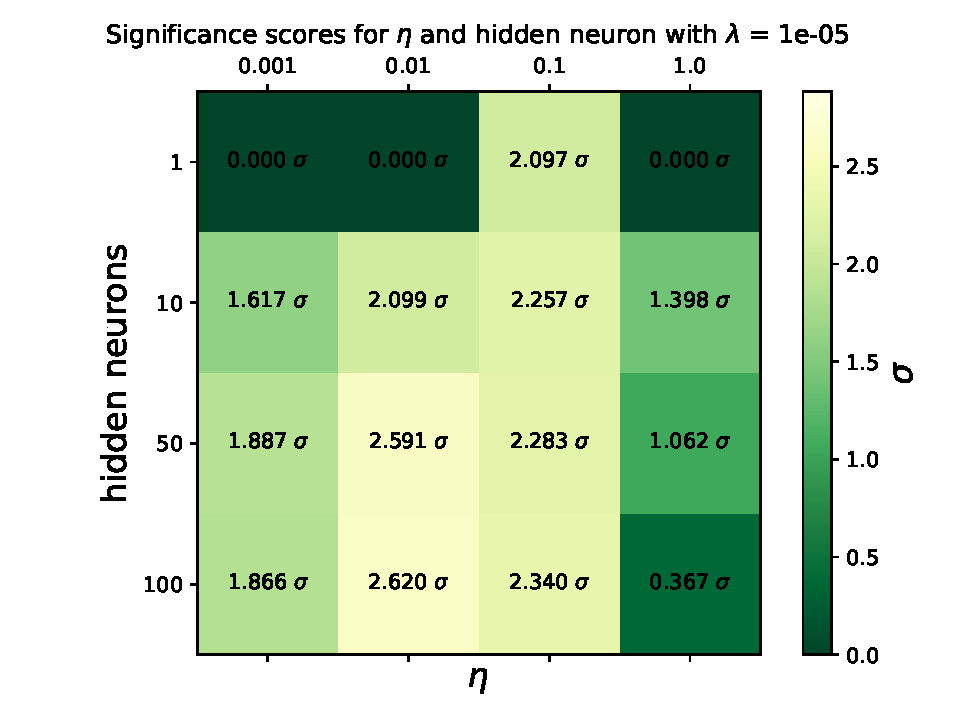
\includegraphics[width=0.6\textwidth]{Significance_ne.pdf}
      \caption{Grid search significance with $\lambda=10^{-5}$ and n\_layers = 2}\label{fig:NN_GRID_SIG}
\end{figure}
\graphicspath{{../../../Plots/NeuralNetwork/FULL/GRID_lamda_eta_neurons/AUC}}
\begin{figure}[!ht]
	\centering
	\begin{subfigure}[b]{0.49\textwidth}
        \centering
        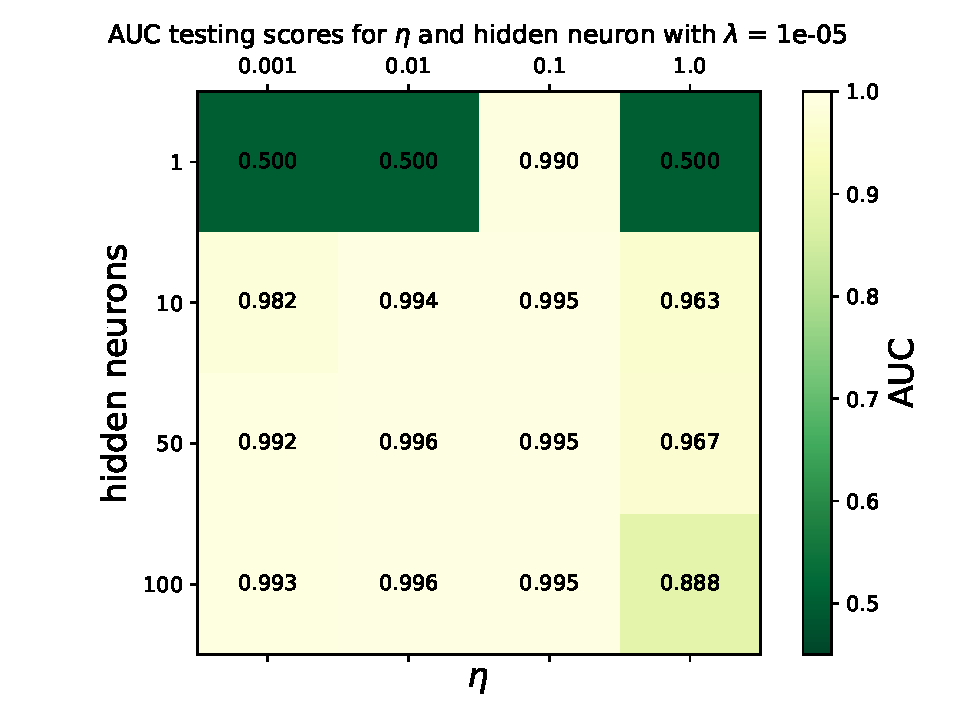
\includegraphics[width=1\textwidth]{testing_ne.pdf}
        \caption{Testing AUC}
     \end{subfigure}
     \hfill
     \begin{subfigure}[b]{0.49\textwidth}
        \centering
        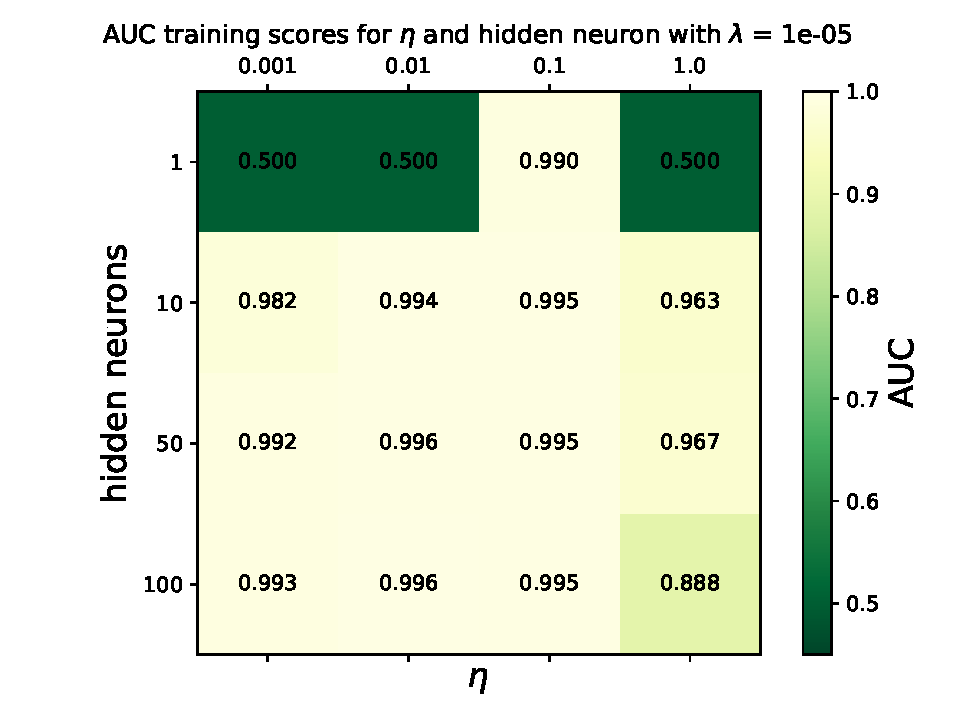
\includegraphics[width=1\textwidth]{training_ne.pdf}
        \caption{Training AUC}
     \end{subfigure}
     \caption{Grid search AUC with $\lambda=10^{-5}$ and n\_layers = 2}\label{fig:NN_GRID_AUC}
\end{figure}
\newpage\noindent Doing the same but with more hidden layers and setting $\lambda=10^{-5}$ we get the results shown in GitHub under \verb|Plots/NeuralNetwork/FULL/GRID_layers_eta_neurons|, 
for the sake of this thesis not being too long I will again only show the significance plot as well as the AUC for the testing and training set but this time when setting $\eta=0.01$. 
The significance is seen in Figure \ref{fig:DNN_GRID_SIG}, while the AUC is in Figure \ref{fig:DNN_GRID_AUC}. 
\graphicspath{{../../../Plots/NeuralNetwork/FULL/GRID_layers_eta_neurons}}
\begin{figure}[!ht]
      \centering
      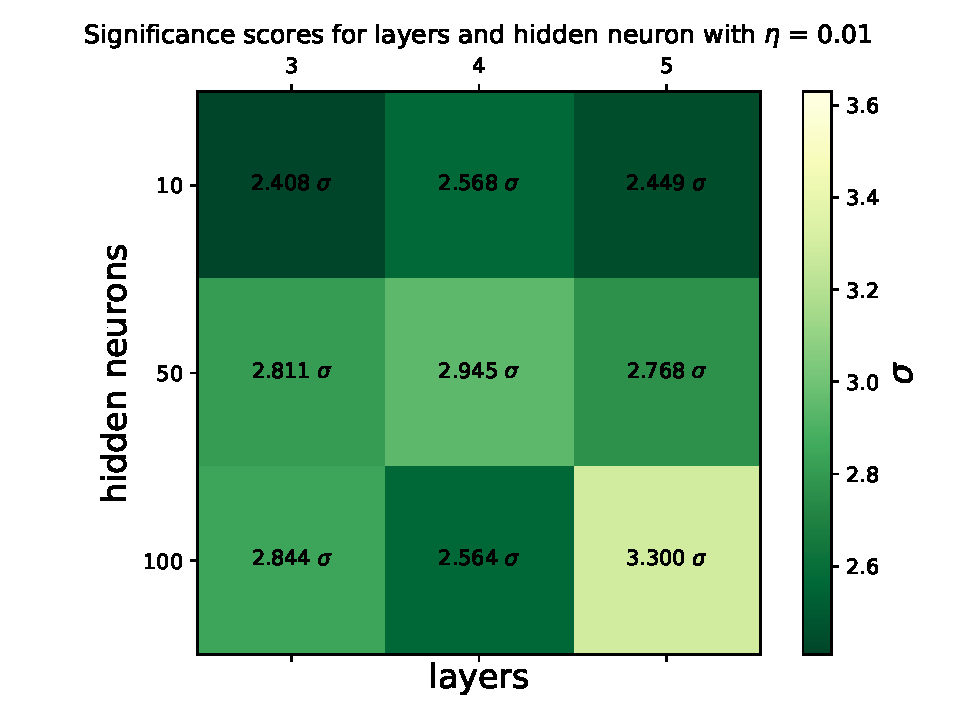
\includegraphics[width=0.6\textwidth]{Significance_nl.pdf}
      \caption{Grid search significance with $\lambda=10^{-5}$ and and $\eta = 0.01$}\label{fig:DNN_GRID_SIG}
\end{figure}

\graphicspath{{../../../Plots/NeuralNetwork/FULL/GRID_layers_eta_neurons/AUC}}
\begin{figure}[!ht]
	\centering
	\begin{subfigure}[b]{0.49\textwidth}
        \centering
        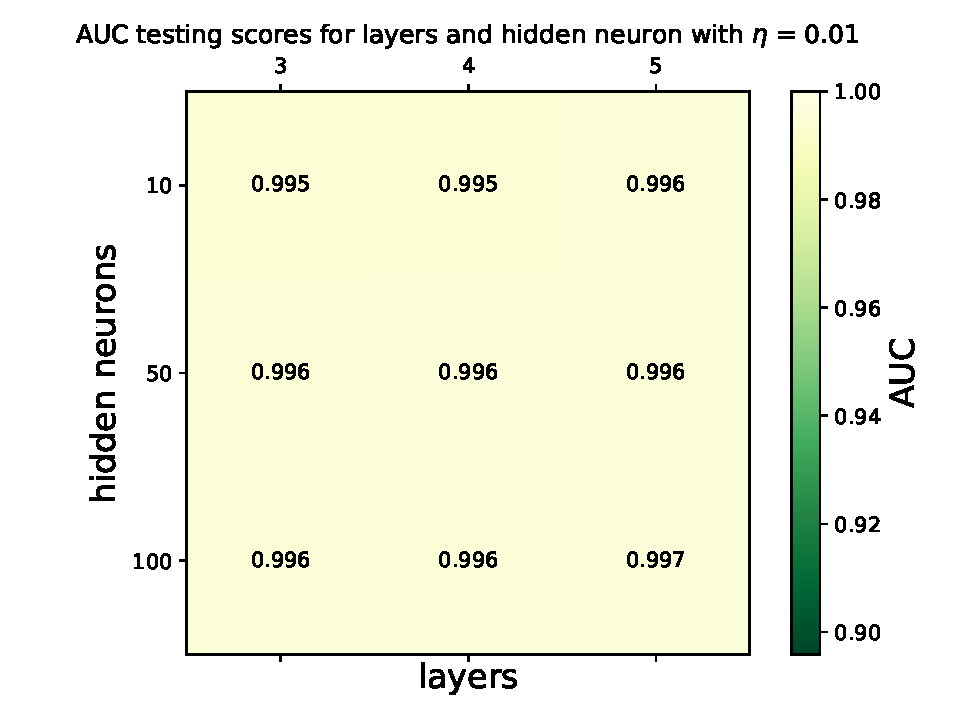
\includegraphics[width=1\textwidth]{testing_nl.pdf}
        \caption{Testing AUC}
     \end{subfigure}
     \hfill
     \begin{subfigure}[b]{0.49\textwidth}
        \centering
        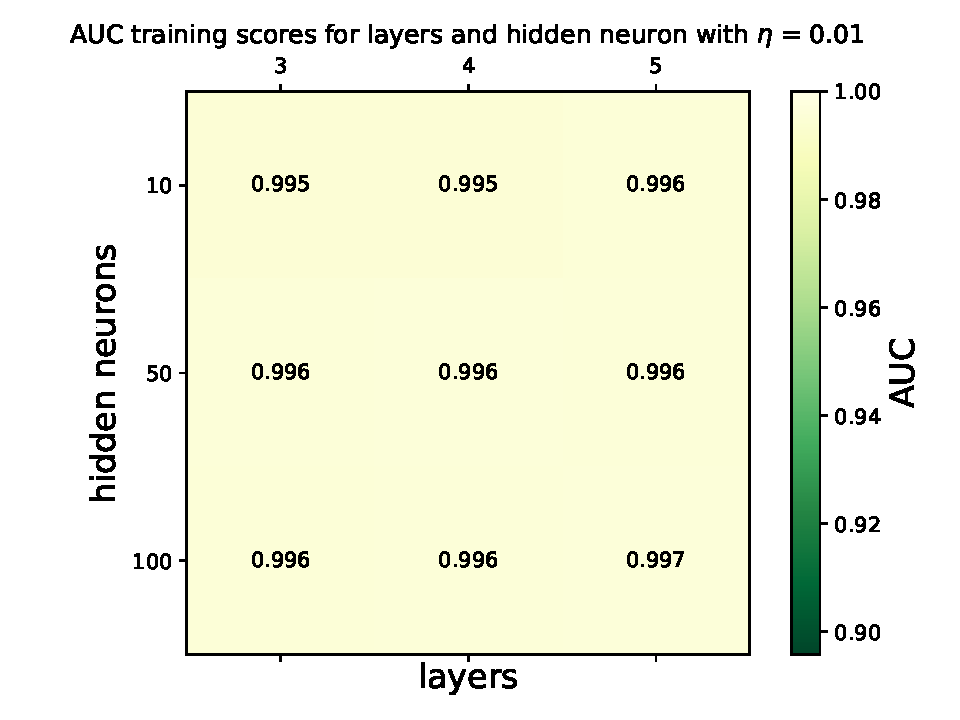
\includegraphics[width=1\textwidth]{training_nl.pdf}
        \caption{Training AUC}
     \end{subfigure}
     \caption{Grid search significance with $\lambda=10^{-5}$ and $\eta = 0.01$}\label{fig:DNN_GRID_AUC}
\end{figure}
\newpage\noindent I also made a test network with the same hyperparameters as the best one in Figure \ref{fig:DNN_GRID_SIG}, the only difference being that it has 10 hidden layers.
I plotted the validation data to see how different the networks were at predicting the DH HDS $m_{Z'}=130$ GeV model. 
These were trained and tested when using the Z-score normalization, Eq. (\ref{eq:Z-score}), and the weighting method explained in section \ref{sec:wgts}. The results are shown in the figure below.
\graphicspath{{../../../Plots/DeepNeuralNetwork/FULL/BEST_GRID/DH_HDS_mZp_130/}}
\begin{figure}[!ht]
	\centering
	\begin{subfigure}[b]{0.49\textwidth}
        \centering
        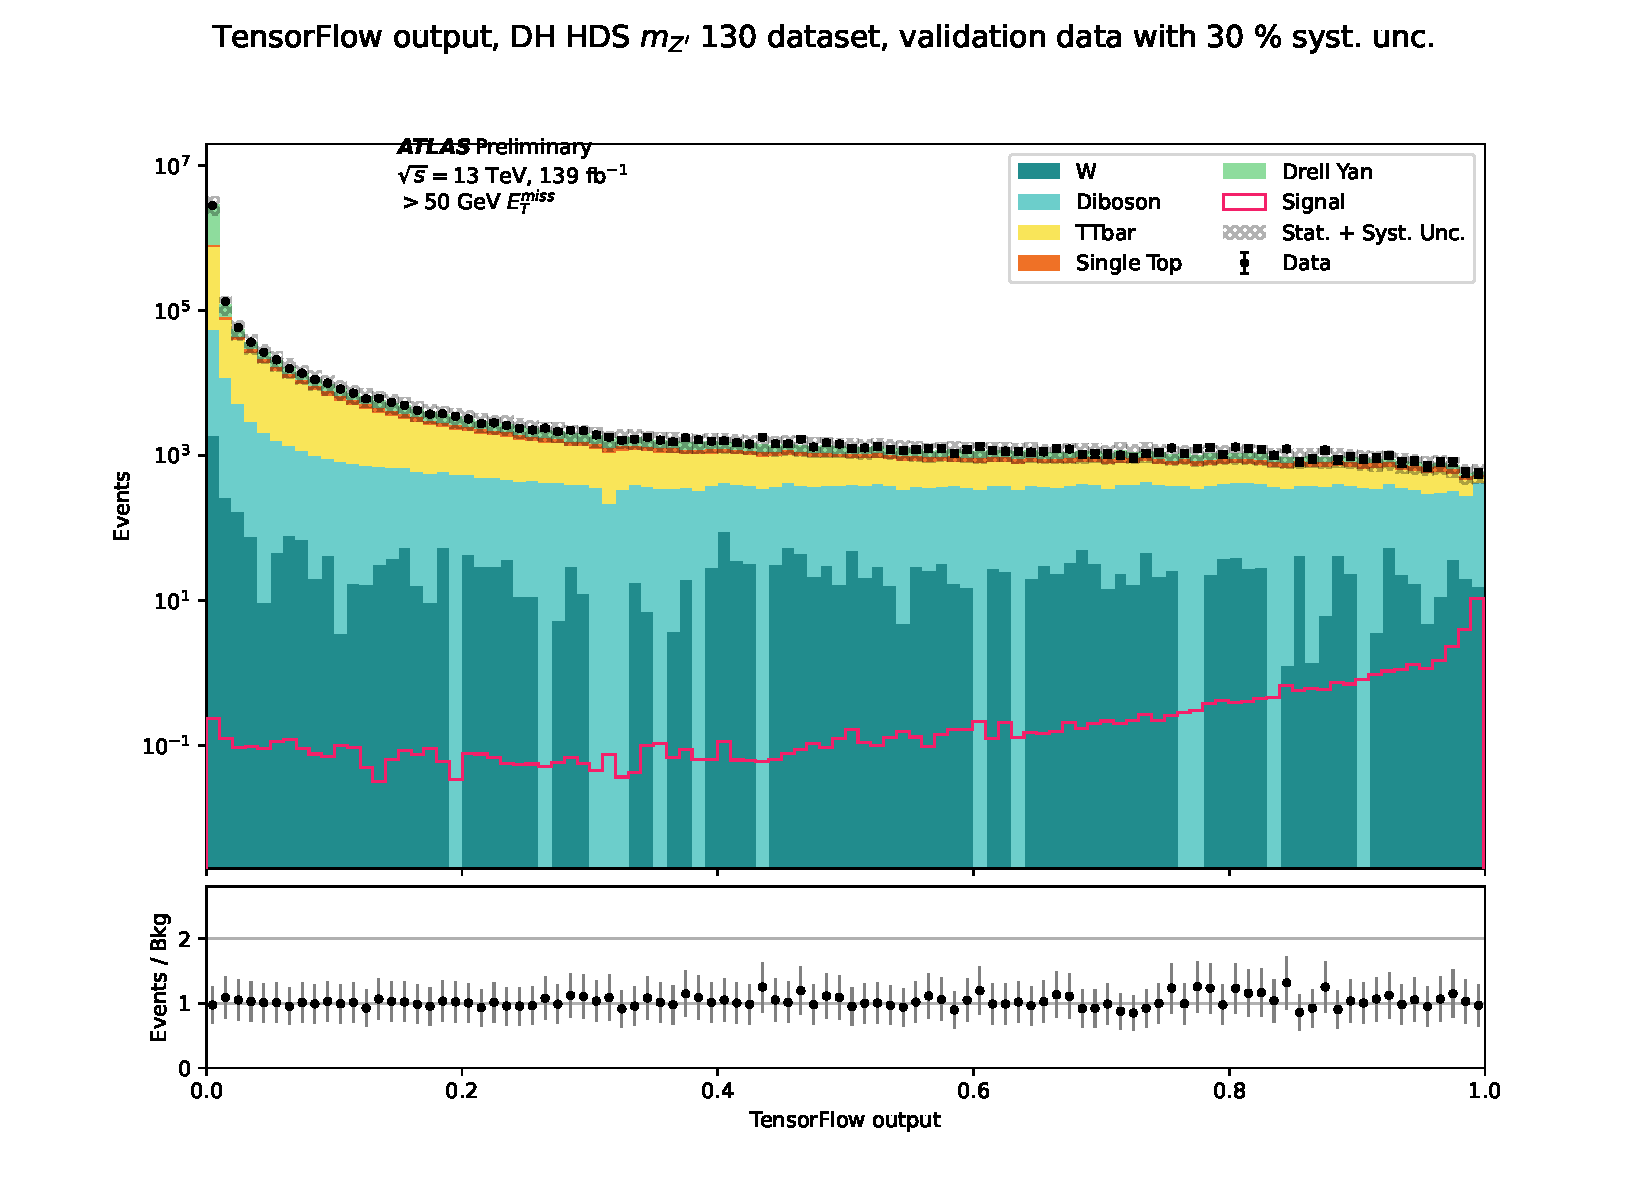
\includegraphics[width=1\textwidth]{VAL.pdf}
        \caption{Four hidden layers}
     \end{subfigure}
     \hfill\graphicspath{{../../../Plots/DeepNeuralNetwork/FULL/10_HIDDEN_LAYERS/DH_HDS_mZp_130/}}
     \begin{subfigure}[b]{0.49\textwidth}
        \centering
        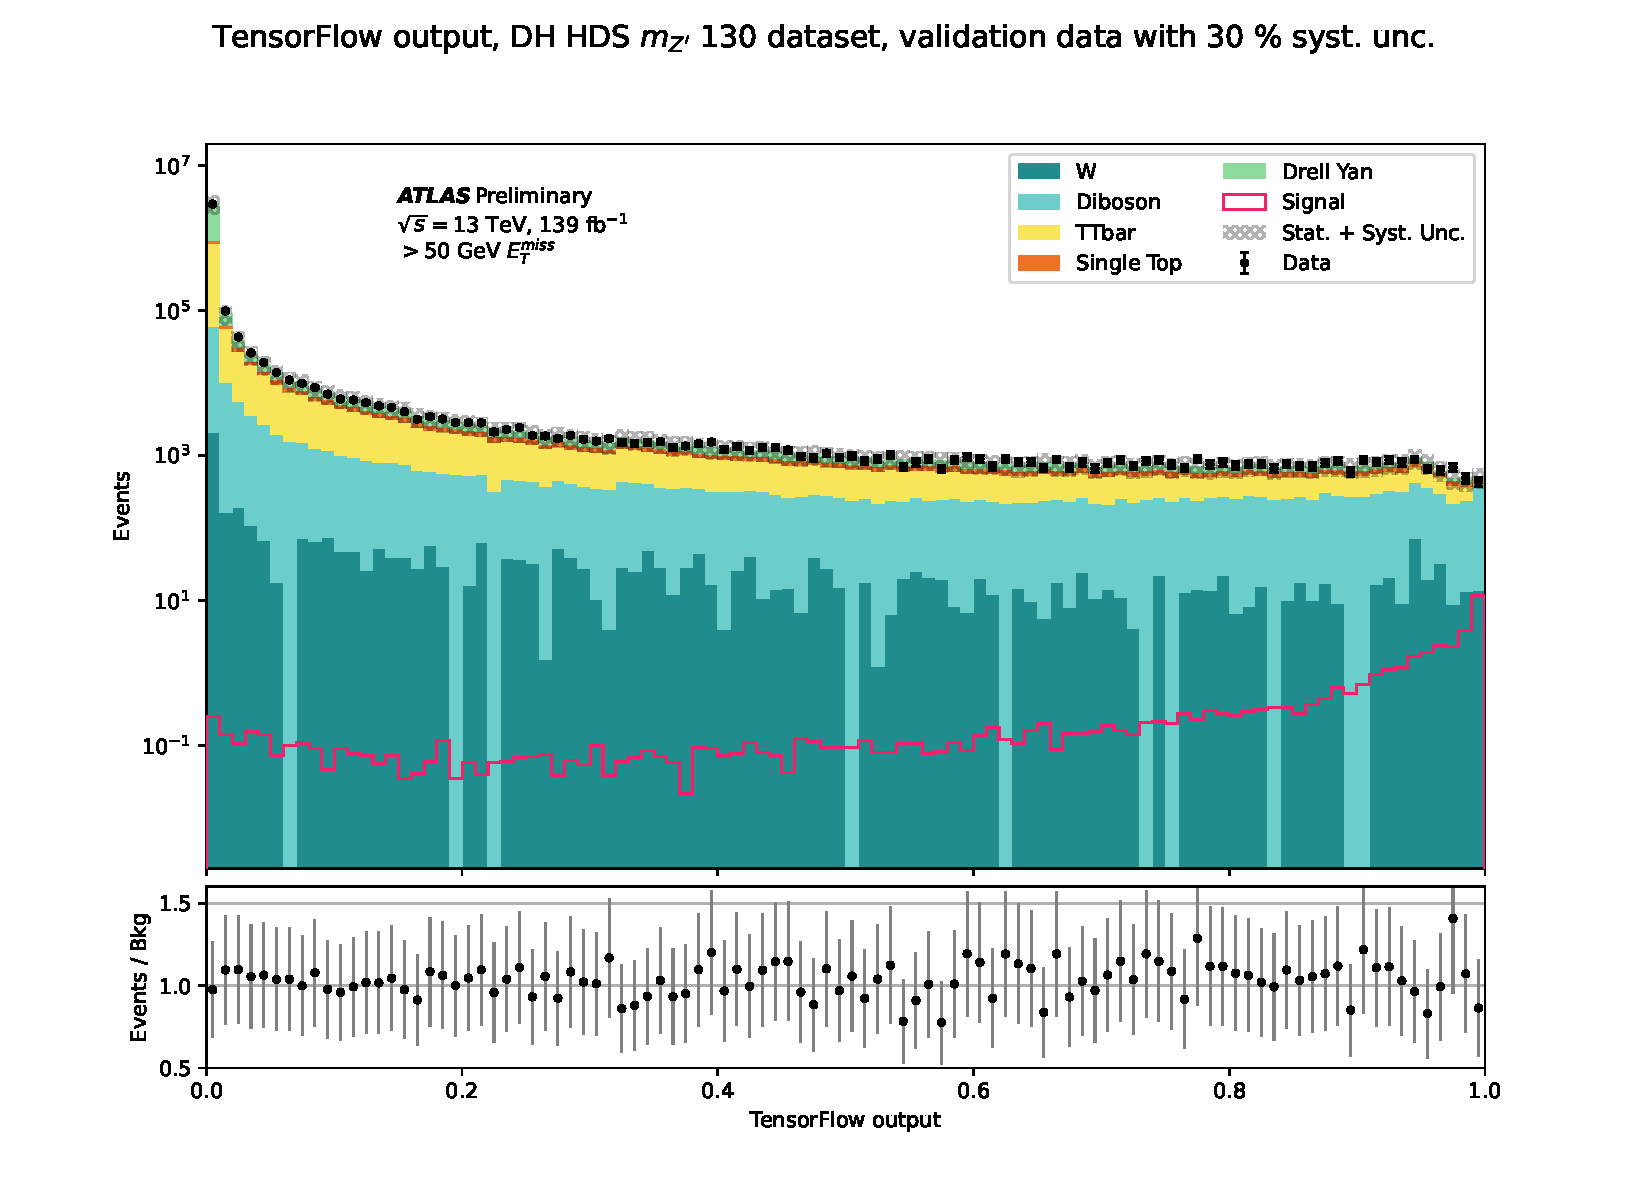
\includegraphics[width=1\textwidth]{VAL.pdf}
        \caption{Ten hidden layers}
     \end{subfigure}
   \hfill\graphicspath{{../../../Plots/DeepNeuralNetwork/FULL/BEST_GRID/DH_HDS_mZp_130/}}
   \begin{subfigure}[b]{0.49\textwidth}
      \centering
      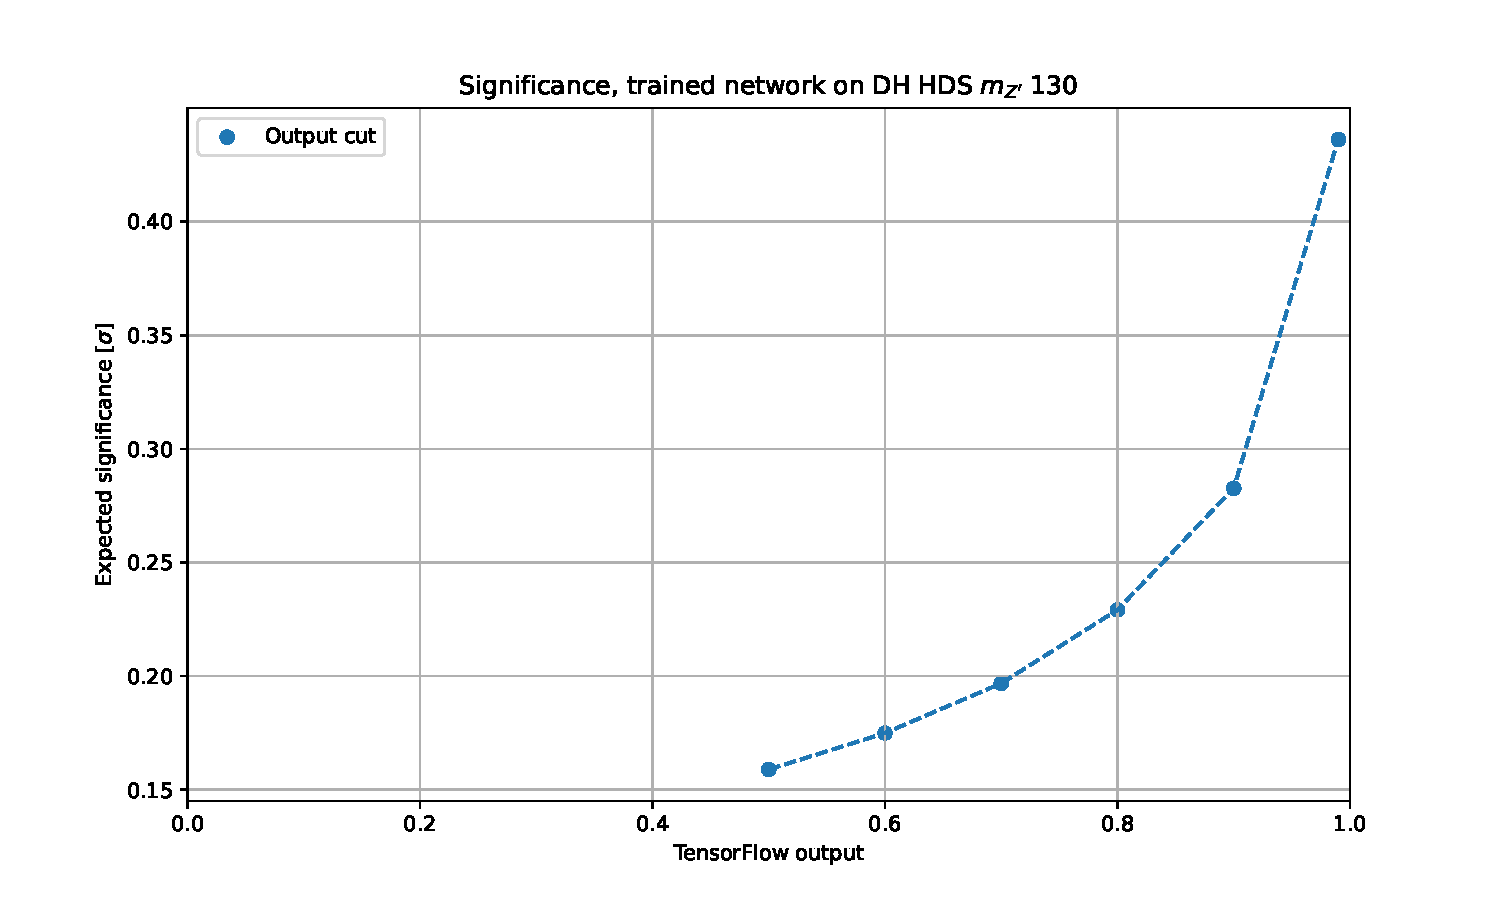
\includegraphics[width=1\textwidth]{EXP_SIG.pdf}
      \caption{The expected significance of a)}
   \end{subfigure}
   \hfill\graphicspath{{../../../Plots/DeepNeuralNetwork/FULL/10_HIDDEN_LAYERS/DH_HDS_mZp_130/}}
   \begin{subfigure}[b]{0.49\textwidth}
      \centering
      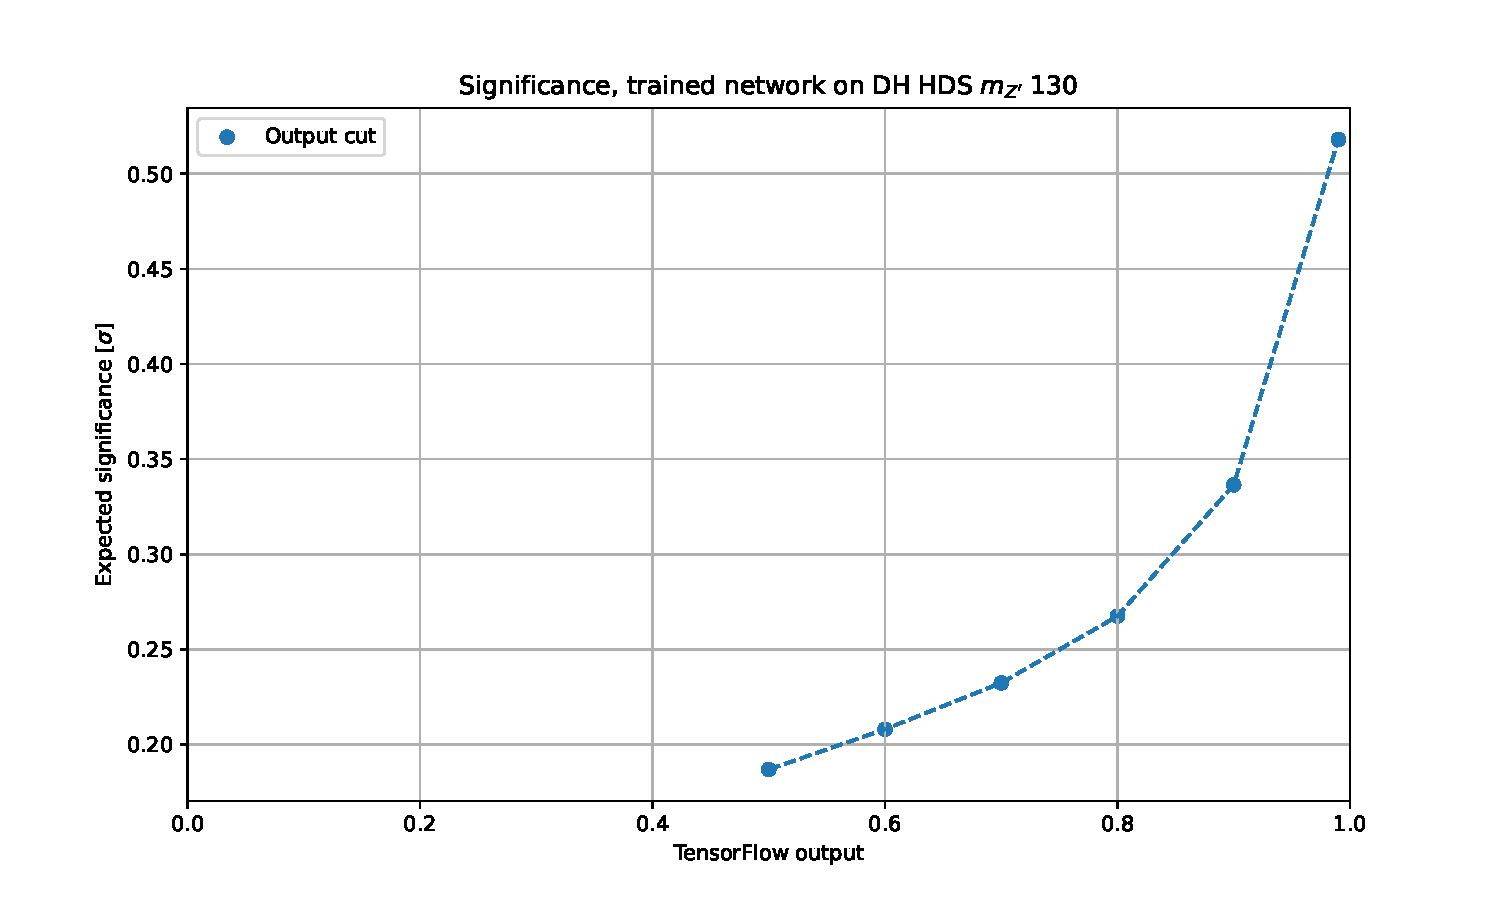
\includegraphics[width=1\textwidth]{EXP_SIG.pdf}
      \caption{The expected significance of b)}
   \end{subfigure}
     \caption{Comparison of the network performance when having four and ten hidden layers. Figure a) and b) show the validation data of both cases, c) and d) show the expected significance of the validation plots when making a cut on the output. }
\end{figure}
\newpage\noindent This hints that we could be able to make a DNN with more hidden layers and get better results. However there are a few things that need to be noted when doing this, aside from the padding which is an even greater problem.
The first and smallest one is that we could have used batch normalization instead of Z-score, but this is again something to be further discussed.\\
\\The second being that I have not used the "balanced weighting" method when training the network, which might be for better or worse if the network really does ignore all EFT models...\\
\\The third one which is more technical is that since more complex networks require more computational power, then this leads to us decreasing the batch size. Which lowers the statistics of signal, 
and might even lead to the network training on batches without any signal sample at all. So the trade off is also something to be discussed.\\
\\The last thing to be noted is that having a DNN completely removes the possibility of combining the results of multiple networks trained on a single model, as the imbalance becomes too much for the network to see anything.
A solution to this however, is that instead of combining the results of multiple networks trained on a singular model, one could try the Parametrized NN approach, which could potentially avoid the imbalance problem, but this is 
proposed as a plausible new research project due to time constrain on this thesis.
\clearpage
\graphicspath{{../../figures/}}






\section{Boosted Desicion Tree Training}
When working with BDTs we do not run into as many problems as we do with NNs. For example the padding and normalization of data can be completely avoided, making the whole procedure a lot easier when one uses "weird data" as we do in HEPP.
There is however one other problem that need to be dealt with when working with this type of ML, this is the weights, which will be discussed in the next section.\\
\\For this project we will as mentioned \todo{remember to mention it} utilize the Extreme Gradient Boosting, or XGBoost for short, package made for the HiggsML\todo{add source/remove this comment?} whenever we mention BDTs.
This project utilized version \verb|1.5.0| without GPU adaptability. XGBoost also helps to avoid padding as it is integrated with a \verb|missing_variable| variable where we can simply write the number of the variable that is missing.

\subsection{Weights}
For XGBoost there is a different problem when it comes to weights. XGBoost has a variable called \verb|scale_pos_weight| where we can help the network deal with unbalanced data, such as the one we have. 
Meaning that the whole problem of section \ref{sec:Balanced_wgts} completely dissapears, meaning we could use the \textit{real} weights calculated in the MC generators.
Sadly it is not that easy, XGBoost does not have to possibility to include negative weights, which this dataset has a few of. Some MC generators generate events with negative weights, such as Sherpa \todo{cite sherpa?}, that take into acount higher order diagrams and needs to add 
negative weights to "counter" the overcounting of diagrams \cite{Negative_Weights_article}, which are important to correctly scale the simulated events to real data.
In the future this might no longer be a problem as \todo{I have no other sources to this other than spoken words at conferenes...} future MC generators might only have positive weights.\\
\\A method to mitigate this problem is to use the absolute value of the weights when training to solve, or rather avoid, this problem. 
This is however not generally accepted as a solution, and some even say it should be avoided. There are other options however, one is to not include events with negative weights on the training set. \\
\\Another one that has been used on a published ATLAS (internal) article (chapter 9.3) \cite{Abbott:2714377} is to normalize the weights when using the absolute value with respect to the sum of weights over the sum of absolute weights. The reason behind this is because the sum of weights is obviously not the same when we take the absolute value. 
Mathemathically speaking, if we have an array of weights $W$, we can update this like
\begin{equation}\label{eq:ATLAS_wgt}
   W \rightarrow \abs{W}\frac{\sum_i W_i}{\sum_i\abs{W_i}}
\end{equation}
such that the weights are at least in the same scale. I have tried all of these options and the results can be seen in Figure \ref{fig:BDT_wgts}.\\
\\As we can see it makes a significant difference whether we use the weights to re-weight MC events to expected events. But there is no mathematical reason as to why we should 
include this re-weighting weight as sample weights, as the reason to use sample weights is to \textit{only} balance signal and bacgkround. In theory it makes no sense whatsoevert to include these weights either 
as the network doesn't really care for cross sections or luminosity, and what we are doing in principle is making it harder for the network to learn anything. But as seen on the results, the BDT learns the background 
extremely well when using the weights, while it also does a poorer job in learning the signal we are testing.\\ 
\\In a sense this is not a negative thing for our purposes, but stricly speaking we are invoking a semi-unsupervised learning method by punishing the network if it learns the signal too quickly. 
To get to the point as why this is good for our purposes, we are indirectly making our network more model indepentent! Because of this, the method that will be pursued further in this thesis will be to 
take the positive weights and balance the data.\todo{Add that ATLAS used it, so because of that so can I?}

\graphicspath{{../../../Plots/XGBoost/WEIGHT_TEST/DH_HDS_mZp_130/}}
\begin{figure}[!ht]
	\centering
	\begin{subfigure}[b]{0.49\textwidth}
      \centering
      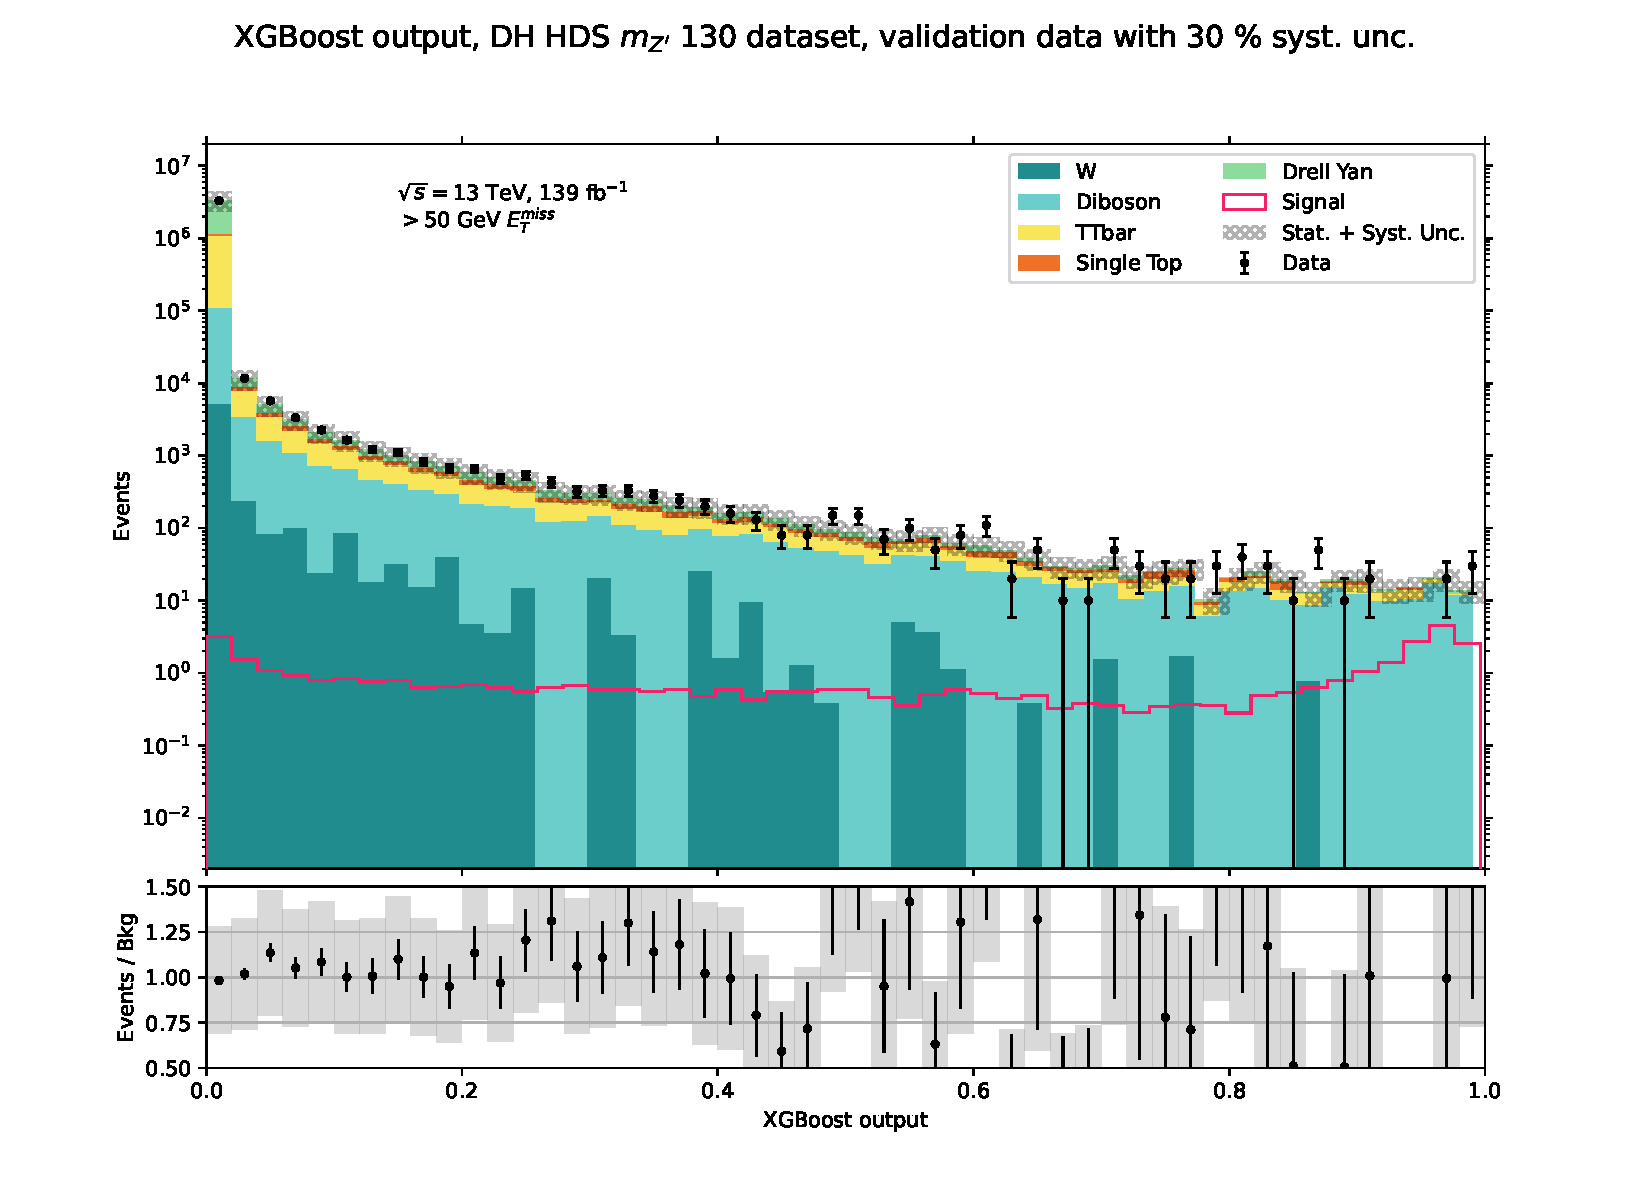
\includegraphics[width=1\textwidth]{ATLAS_ABS/VAL.pdf}
      \caption{Using the scaled absolute value of the weights}
   \end{subfigure}
   \begin{subfigure}[b]{0.49\textwidth}
      \centering
      \includegraphics[width=1\textwidth]{POS/VAL.pdf}
      \caption{Using only positive weights}
   \end{subfigure}
   \begin{subfigure}[b]{0.49\textwidth}
      \centering
      \includegraphics[width=1\textwidth]{NONE/VAL.pdf}
      \caption{Using no weights}
   \end{subfigure}
   \caption{Difference when using different weighting methods. All networks were trained using the balancing method explained in Section \ref{sec:wgts}}\label{fig:BDT_wgts}
\end{figure}


% \subsection{General structure of the network}
% BDT illustration? \\
% \\Makinga BDT for our purposes is fairly easy as well using XGBoost. One way to do it is using the code below in Algorithm
% \begin{lstlisting}[language=Python, caption={Boosted Decision Tree definition using XGBoost}, label=alg:xgb, captionpos=t]
%    import xgboost as xgb
   
%    Boosted_Decision_Tree = xgb.XGBClassifier(
%                 max_depth, 
%                 use_label_encoder=False,
%                 n_estimators,
%                 learning_rate,
%                 reg_lambda,
%                 predictor = 'cpu_predictor',
%                 tree_method = 'hist',
%                 scale_pos_weight=sow_bkg/sow_sig,
%                 objective='binary:logistic',
%                 eval_metric='auc',
%                 missing=10,
%                 random_state=42,
%                 verbosity = 1) 
% \end{lstlisting}


\clearpage
\subsection{Grid Search}\label{sec:BDTGriddy}
To get the best performance on our BDT we have to do a grid search here as well. The trainable hyperparameters here are different than for NNs though. 
With XGBoost we have the following hyperparameters
\begin{itemize}
   \item Tree depth: how many times we split the data
   \item Number of estimators: how many estimators we use to do out gradient boosting
   \item The learning rate $\eta$
   \item L2-regressor $\lambda$, to stop overtraning
\end{itemize}
The data set used for this grid search is the same one used in the NN grid search. That is the FULL Z' DM data set containing DH, LV and EFT models. 
The metrics used to evaluate the score for this case was again the \textbf{AUC} and \textbf{expected significance}. One thing to note, for this section I did not include the weighting method showcased in the previous section,
I only used the data balancing method, as this is its intended purpose.\\
\\At first I set the number of estimators to be 120 and fixed the L2 $\lambda$ to $10^{-5}$. Then conducted a grid search on the tree depth and learning rate only. 
I used the same range on the learning rate as I did with the NNs, $\eta \in [0.001, 0.01, 0.1, 1]$, and first did a treee depth from 3-6. 
This showed however a trend hinting to the expected significance only increasing with more depth, because of this I ended up continuing the grid search up to a depth of 30.
The results can be shown in Figure \ref{fig:BDT_deep_sig}. This is however highly radical as the convention is to normally not have a depth greater than 7, 
the reason being that the network is highly likely to overtrain and give wrong predictions. However this was not the case for me as seen for example in Figure \ref{fig:DBDT_GRID_AUC}.
\graphicspath{{../../../Plots/XGBoost/FULL/GRIDSEARCH_3-6}}
\begin{figure}[!ht]
	\centering
	\begin{subfigure}[b]{0.49\textwidth}
      \centering
      \includegraphics[width=1\textwidth]{Expected_significance.pdf}
   %   \caption{Testing AUC}
   \end{subfigure}
   \hfill\graphicspath{{../../../Plots/XGBoost/FULL/GRIDSEARCH_24-30}}
   \begin{subfigure}[b]{0.49\textwidth}
      \centering
      \includegraphics[width=1\textwidth]{Expected_significance.pdf}
   %   \caption{Training AUC}
   \end{subfigure}
   \caption{Grid search expected significance going to a depth of up to 30}\label{fig:BDT_deep_sig}
\end{figure}
\graphicspath{{../../../Plots/XGBoost/FULL/GRIDSEARCH_24-30}}
\begin{figure}[!ht]
\centering
\begin{subfigure}[b]{0.49\textwidth}
      \centering
      \includegraphics[width=1\textwidth]{Testing_AUC.pdf}
      \caption{Testing AUC}
   \end{subfigure}
   \hfill
   \begin{subfigure}[b]{0.49\textwidth}
      \centering
      \includegraphics[width=1\textwidth]{Training_AUC.pdf}
      \caption{Training AUC}
   \end{subfigure}
   \caption{Grid search AUC going to a depth of up to 30}\label{fig:DBDT_GRID_AUC}
\end{figure}
\\ I understand however that this is controversial since we are splitting a data set, that is at best of size $2^{27}$, 30 times. That means that after a depth of 27 there is exaclty one event pr branch.
So how does a depth of 30 make sense? To help with this we could use a feature in XGBoost to see which features are most important when evaluating a signal. 
When testing the network trained on the FULL Z' DM data set on a DH HDS $m_{Z'}=130$ GeV model we get the features shown in Figure \ref{fig:DBDT_feat} as most important. 
\graphicspath{{../../../Plots/XGBoost/FULL/DH_HDS_mZp_130/feature_importance}}
\begin{figure}[!ht]
	\centering
   \begin{subfigure}[b]{0.8\textwidth}
      \centering
      \includegraphics[width=1\textwidth]{weight.pdf}
      \caption{Using "weight" metric}
   \end{subfigure}
   \hfill
   \begin{subfigure}[b]{0.8\textwidth}
      \centering
      \includegraphics[width=1\textwidth]{total_cover.pdf}
      \caption{Using "coverage" metric}
   \end{subfigure}
   \caption{Feature importance of depth 30 network trained on FULL Z' DM data set when testing it on DH HDS $m_{Z'}=130$ GeV model.}\label{fig:DBDT_feat}
\end{figure}
\newpage\noindent As we can see these features vary a lot depending on which metric we use to evaluate the importance. 
When using the "coverage" metric, which as stated is defined as the number of samples affected by the split, we get the features we physically expect to be important when trying to single out a DM model.
And this metric is arguably the one we need to use to define what features are important. Since the more samples a feature split, the more powerful it is to separate signal from background.\\
\\We can see however that when we use "weight" as a metric, which is the XGBoost standard metric, we get completely unexpected features that we physically don't expect to be important when trying to single out a DM model.
But as described by the metric, the "weight" is the number of times a feature appears in a tree. Which might explain that the reason the pseudorapidity and $\phi$ range so high on this list, 
is simply because the tree is struggling to find a pattern here and is trying extra hard to single out DM from SM. \\
\newpage\noindent As the previous results are to be taken with a heavy grain of salt, I conducted another grid search. On the second grid search I set the values of $\eta=0.1$ as the trend showed this giving the best results with less overtraining, 
and $\lambda=10^{-5}$ \todo{should I conduct a new grid search with different $\lambda$ and loss functions?}. This grid search had \verb|n_estimators| $\in[10, 100, 500, 1000]$ and depth $\in[3,4,5,6]$. 
The expected significance is shown in Figure \ref{fig:BDT_sig}. The testing and training AUC can be seen in Figure \ref{fig:BDT_GRID_AUC}.
\graphicspath{{../../../Plots/XGBoost/FULL/GRIDSEARCH_n_est_10-1000}}
\begin{figure}[!ht]
   \centering
   \includegraphics[width=0.6\textwidth]{Expected_significance.pdf}  
   \caption{Grid search expected significance when setting $\lambda=10^{-5}$ and $\eta=0.1$}\label{fig:BDT_sig}
\end{figure}
\begin{figure}[!ht]
\centering
\begin{subfigure}[b]{0.49\textwidth}
      \centering
      \includegraphics[width=1\textwidth]{Testing_AUC.pdf}
      \caption{Testing AUC}
   \end{subfigure}
   \hfill
   \begin{subfigure}[b]{0.49\textwidth}
      \centering
      \includegraphics[width=1\textwidth]{Training_AUC.pdf}
      \caption{Training AUC}
   \end{subfigure}
   \caption{Grid search AUC when setting $\lambda=10^{-5}$ and $\eta=0.1$}\label{fig:BDT_GRID_AUC}
\end{figure}
\\When testing the best network with a depth of 6 and 1000 estimators on the same DH HDS $m_{Z'}=130$ GeV model we get the feature importance plots shown in Figure \ref{fig:BDT_feat}. 
Here we see that the "weight" metric gives us the expected features as most important. But the "cover" metric seems to be less of what we expect since the jet kinematic variables score higher, 
this might just be a curiosity rather than something to be suspect of.
\graphicspath{{../../../Plots/XGBoost/FULL/GRIDSEARCH_n_est_10-1000/DH_HDS_mZp_130/feature_importance/}}
\begin{figure}[!ht]
	\centering
   \begin{subfigure}[b]{0.8\textwidth}
      \centering
      \includegraphics[width=1\textwidth]{weight.pdf}
      \caption{Using "weight" metric}
   \end{subfigure}
   \hfill
   \begin{subfigure}[b]{0.8\textwidth}
      \centering
      \includegraphics[width=1\textwidth]{total_cover.pdf}
      \caption{Using "coverage" metric}
   \end{subfigure}
   \caption{Feature importance of depth 30 network trained on FULL Z' DM data set when testing it on DH HDS $m_{Z'}=130$ GeV model.}\label{fig:BDT_feat}
\end{figure}

\clearpage\noindent To showcase the difference in signal recognition between the monstrous 30 depth BDT to the more sensible 6 depth BDT, I again tested the networks on the good old DH HDS $m_{Z'}=130$ GeV model.
The results as well as their expected significance can be seen below.
\begin{figure}[!ht]
	\centering
   \graphicspath{{../../../Plots/XGBoost/FULL/GRIDSEARCH_n_est_10-1000/DH_HDS_mZp_130/}}
	\begin{subfigure}[b]{0.49\textwidth}
        \centering
        \includegraphics[width=1\textwidth]{VAL.pdf}
        \caption{Depth of 6}
     \end{subfigure}
     \hfill\graphicspath{{../../../Plots/XGBoost/FULL/DH_HDS_mZp_130/}}
     \begin{subfigure}[b]{0.49\textwidth}
        \centering
        \includegraphics[width=1\textwidth]{VAL.pdf}
        \caption{Depth of 30}
     \end{subfigure}
   \hfill\graphicspath{{../../../Plots/XGBoost/FULL/GRIDSEARCH_n_est_10-1000/DH_HDS_mZp_130/}}
   \begin{subfigure}[b]{0.49\textwidth}
      \centering
      \includegraphics[width=1\textwidth]{EXP_SIG.pdf}
      \caption{The expected significance of a)}
   \end{subfigure}
   \hfill\graphicspath{{../../../Plots/XGBoost/FULL/DH_HDS_mZp_130/}}
   \begin{subfigure}[b]{0.49\textwidth}
      \centering
      \includegraphics[width=1\textwidth]{EXP_SIG.pdf}
      \caption{The expected significance of b)}
   \end{subfigure}
   \caption{Comparison of the network performance when having a depth of 6 and 30. Figure a) and b) show the validation data of both cases, c) and d) show the expected significance of the validation plots when making a cut on the output. }
\end{figure}
\\The difference is extreme, when looking at the monster of depth 30 we can get an expected significance of 1.2 $\sigma$ (without uncertainties)\todo{when should I use them?} on our model of max 15 events, only having made a cut of 50 GeV on the missing transverse energy.
We can however see that the data and background do not agree to the same degree of the network with depth 6. Using purely statistical uncertainty and assuming a systematic uncertainty of 30\%, we see that a few data ponts do not agree with the MC background.
These data points are points the network classified as signal, so if we completely trusted the network this would be a hint of new physics! 
However this is the last thing we should assume, and rather take this as a hint that the network is doing something fishy.\\
\\If I had access to XGBoost with built GPU support, I would increase the number of estimators even more to check if this increases the significance while still having a depth of maximum 6.
However as of now this is not possible. As the weighting method explained in the previous section was not included here, we will drop going to a tree depth of 30, and have a maximum of 6.

\end{document}